% !TEX root = master_thesis.tex

\chapter{Extraction of the beam asymmetries $\Sigma_{\eta}$ and $\Sigma_{\eta'}$}
The beam asymmetry $\Sigma$ can be measured from data taken with a linearly polarized photon beam and an unpolarized liquid hydrogen target \cite{san}. The polarized differential cross section $\frac{\text{d}\sigma}{\text{d}\Omega}_\text{pol}$ is not uniformly distributed in the azimuthal angle $\phi$ anymore as opposed to the unpolarized diffenrential cross section $\frac{\text{d}\sigma}{\text{d}\Omega}_0$. It is rather modulated by a cosine dependence which scales with the polarization observable $\Sigma$ and the (linear) beam polarization $p_\gamma$, see equation \eqref{eq:asym} \cite{san}.
\begin{equation}
	\frac{\text{d}\sigma}{\text{d}\Omega}_\text{pol}\left(E_\gamma,\cos\theta,\phi\right)=\frac{\text{d}\sigma}{\text{d}\Omega}_0\left(E_\gamma,\cos\theta\right)\cdot\left[1-p_\gamma\Sigma\left(E_\gamma,\cos\theta\right)\cos\left(2\varphi\right)\right]
	\label{eq:asym}
\end{equation}
Since the incident photon beam is polarized, photon momentum $\vec{k}$ and polarization $\vec{\epsilon}$ span a plane which is referred to as the beam polarization plane. This plane is tilted by the angle $\varphi$ with respect to the reaction plane which is defined by the final state momenta. Naturally, this plane builds the angle $\phi$ in the laboratory system. At the same time the angle of the beam polarization plane in the same reference frame is defined as $\alpha$. It holds 
\begin{equation}
	\varphi=\alpha-\phi.
\end{equation} Figure \ref{fig:angles} illustrates definitions of all angles and planes. 
 \begin{figure}[htbp]
	\centering
	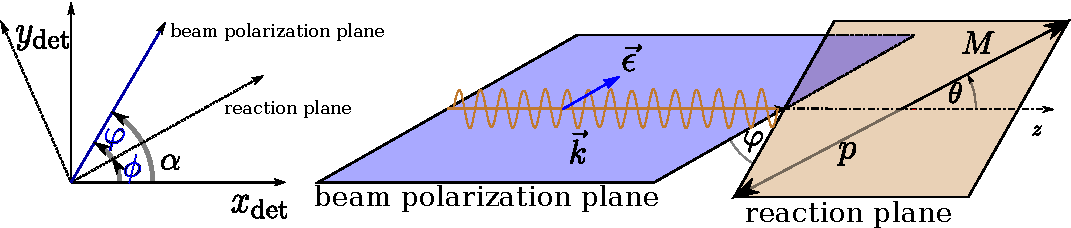
\includegraphics[width=\linewidth]{../DPG2022/figs/angles.pdf}
	\caption{Left: Definition of the angles $\alpha,\phi,\varphi$. Right: Photon momentum $\vec{k}$ and polarization  $\vec{\epsilon}$ define the beam polarization plane while the reaction plane is defined by the recoil proton $p$ and produced meson $M$.}
	\label{fig:angles}
\end{figure} 
Theoretically the beam asymmetry can be determined by a measurement of the cross section and a fit using equation \eqref{eq:asym}. However, when calculating polarized cross sections, it is important to have good control over flux normalization and detector acceptance in three dimensions $(E_\gamma,\cos\theta,\phi)$ to minimize systematical errors. To avoid this, the measurement of asymmetries can be used to access the polarization observable $\Sigma$ instead. Particularly, data is taken for two distinct orthogonal polarization settings corresponding to $\alpha=\pm\SI{45}{\degree}$.

This chapter will illustrate the process of determining the beam asymmetry for $\eta$ and $\eta'$ photoproduction. The published results of $\Sigma_{\eta}$ \cite{farahphd,eta} are used to check the accuracy and functionality of the employed bayesian methods. Bayesian methods, as well as traditional frequentist approaches are used afterwards to extract new results for $\Sigma_{\eta'}$. First, the determination of the beam photon polarization is briefly described, then the used methods will be presented and subsequently their application for each final state is shown, respectively.
\section{Methods}
\label{sec:meth}
The beam asymmetry has to be determined via fits to asymmetry distributions obtained from data. These are performed as either binned or unbinned fits. Both methods allow the application of Bayesian methods as will be discussed in the following. Additionally the advantages and disadvantages off all methods are compared.
\subsection{Event yield asymmetries}
\label{subsec:evyield}
Measurements were made in two distinct polarization settings $\alpha=\pm\SI{45}{\degree}=\alpha^{\bot/\parallel}$. Thus, the polarized cross sections for both settings are given by\footnote{The dependencies $\left(E_\gamma,\cos\theta,\phi\right)$ of the polarized and the unpolarized cross sections as well as the beam asymmetry like in equation \eqref{eq:asym} are implied.}
\begin{equation}
	\frac{\text{d}\sigma}{\text{d}\Omega}_\text{pol}^\parallel=\frac{\text{d}\sigma}{\text{d}\Omega}_0\cdot\left[1-p_\gamma^\parallel\Sigma\cos\left(2\left(\alpha^\parallel-\phi\right)\right)\right]
	\label{eq:polcs0}
\end{equation}
and 
\begin{align}
	\frac{\text{d}\sigma}{\text{d}\Omega}_\text{pol}^\bot&=\frac{\text{d}\sigma}{\text{d}\Omega}_0\cdot\left[1-p_\gamma^\bot\Sigma\cos\left(2\left(\alpha^\bot-\phi\right)\right)\right]\label{eq:polcs00}\\
	&=\frac{\text{d}\sigma}{\text{d}\Omega}_0\cdot\left[1+p_\gamma^\bot\Sigma\cos\left(2\left(\alpha^\parallel-\phi\right)\right)\right].\label{eq:polcs}
\end{align}
Note that equation \eqref{eq:polcs} holds, because 
\begin{align*}
	\alpha^\bot=\alpha^\parallel+\pi/2 &&\text{and}&&\cos x = -1\cdot\cos(x+\pi).
\end{align*}
Consider now taking the difference of equations \eqref{eq:polcs0} and \eqref{eq:polcs}
\begin{equation}
	\frac{\text{d}\sigma}{\text{d}\Omega}_\text{pol}^\bot-\frac{\text{d}\sigma}{\text{d}\Omega}_\text{pol}^\parallel=\frac{\text{d}\sigma}{\text{d}\Omega}_0\cdot\left(p_\gamma^\bot+p_\gamma^\parallel\right)\Sigma\cos\left(2\left(\alpha^\parallel-\phi\right)\right).
\end{equation}
One can further eliminate the unpolarized cross section from this equation by dividing by the polarization weighted sum of equations \eqref{eq:polcs0} and \eqref{eq:polcs}
\begin{equation}
	\alpha\cdot\frac{\text{d}\sigma}{\text{d}\Omega}_\text{pol}^\bot+\beta\cdot\frac{\text{d}\sigma}{\text{d}\Omega}_\text{pol}^\parallel=\frac{\text{d}\sigma}{\text{d}\Omega}_0\cdot\left[\alpha+\beta-\left(\alpha p_\gamma^\bot-\beta p_\gamma^\parallel\right)\Sigma\cos\left(2\left(\alpha^\parallel-\phi\right)\right)\right]\overset{!}{=}2\frac{\text{d}\sigma}{\text{d}\Omega}_0.
\end{equation}
Since $$\frac{\text{d}}{\text{d}\phi}\frac{\text{d}\sigma}{\text{d}\Omega}_0\overset{!}{=}0\hspace{0.2cm}\forall\phi,$$ it holds \begin{align}
	\alpha p_\gamma^\parallel-\beta p_\gamma^\bot \overset{!}{=}0 && \alpha+\beta\overset{!}{=}2,
\end{align}
such that
\begin{align}
	\alpha =\frac{2p_\gamma^\parallel}{p_\gamma^\bot+p_\gamma^\parallel} && \beta=\frac{2p_\gamma^\bot}{p_\gamma^\bot+p_\gamma^\parallel}.
	\label{eq:alphabeta}
\end{align}
The beam asymmetry $\Sigma$ is thus accessible via the asymmetry \begin{equation}
	A(\phi)=\frac{\frac{\text{d}\sigma}{\text{d}\Omega}_\text{pol}^\bot-\frac{\text{d}\sigma}{\text{d}\Omega}_\text{pol}^\parallel}{p_\gamma^\parallel\frac{\text{d}\sigma}{\text{d}\Omega}_\text{pol}^\bot+p_\gamma^\bot\frac{\text{d}\sigma}{\text{d}\Omega}_\text{pol}^\parallel}=\Sigma\cos\left(2\left(\alpha^\parallel-\phi\right)\right).
	\label{eq:asymfit}
\end{equation}
At this point one can now make use of the fact that in any scattering reaction the number of events $N$ is given by the product of luminosity $L$ and total cross section $\sigma$ \cite{povh} $$N=L\cdot\sigma=\Phi\cdot N_t\cdot\frac{\text{d}\sigma}{\text{d}\Omega}\cdot\Delta\Omega,$$
where $\Phi$ is the beam flux, $N_t$ the number of target particles and $\Delta\Omega$ is the solid angle covered by the detector. Substituting this in equation \eqref{eq:asymfit} one can build the asymmetry $A(\phi)$ using only the (flux-)normalized event yields $\tilde{N}^{\parallel/\bot}\left(E_\gamma,\cos\theta,\phi\right)$\footnote{Again, arguments $\left(E_\gamma,\cos\theta,\phi\right)$ are implied.}
\begin{equation}
	A(\phi)=\frac{\tilde{N}^\bot-\tilde{N}^\parallel}{p_\gamma^\parallel\tilde{N}^\bot+p_\gamma^\bot\tilde{N}^\parallel}=\Sigma\cos\left(2\left(\alpha^\parallel-\phi\right)\right).
	\label{eq:evyieldasym}
\end{equation}
Alternatively, the event yields $N$ can also be normalized by integrating over the total azimuthal angle range in each bin of $(E_\gamma,\cos\theta)$. This normalization technique has been used in reference \cite{farahphd} due to difficulties with the measurement of the photon flux and will also be used in this work. Using appropriate binning in $\phi$ in addition to beam energy and meson polar angle the asymmetry can be build for all kinematic bins and the beam asymmetry then be extracted via a one-parameter \footnote{In general one could still allow an offset to Eq. \ref{eq:evyieldasym} as a second fit parameter. In ref. \cite{farahphd} this was shown to be consistent with $0$.} fit. The statistical errors for $A(\phi)$ are given by \textsc{Gaussian} error propagation (see appendix \ref{sec:stat_err}). 
\subsubsection{Frequentist}
The beam asymmetry can now be determined via a frequentist fit, where $\Sigma$ is determined such that the $\chi^2$ value resulting from the data points and equation \ref{eq:evyieldasym} is minimized. The results are point estimates with statistical error bars that are also obtained from the fit: $\hat{\Sigma}\pm\sigma_{\hat{\Sigma}}$. One can show that the probability distribution of the $\chi^2$ value, given $n$ degrees of freedom, has mean $n$ and variance $2n$ \cite{statistics}. This means $\chi^2/\text{NDF}\approx1$ may be verified in order to diagnose the fit itself. Much larger values indicate a bad fit and much smaller values an overestimation of errors \cite{statistics}. Multiple automated minimization and calculation algorithms for $\chi^2$ fitting are available as open source. The \emph{Python} \cite{python} module \texttt{scipy} \cite{scipy} and \emph{ROOT} \cite{root} offer e.g. the methods \texttt{scipy.optimize.curve\_fit} \cite{pFit} and \texttt{TH1::Fit()} \cite{rFit} for discrete/binned data, which were used in the analysis.
\subsubsection{\textsc{Bayesian}}
Following section \ref{sec:bayes}, where the basics of \textsc{Bayesian} inference were discussed, the goal of a \textsc{Bayesian} approach is to sample marginal posterior distributions for each fitted parameter from the joint posterior $p(\boldsymbol{\theta}|y)$ which depends on the observed data $y$. The joint posterior itself is proportional to the product of priors $\pi(\boldsymbol{\theta})$ and likelihood $\mathcal{L}(y|\boldsymbol{\theta})$ (\textsc{Bayes'} theorem). This collapses to a one parameter problem in the case of fitting the event yield asymmetries (Eq. \eqref{eq:evyieldasym})
\begin{equation}
	p(\Sigma|y)\propto \pi({\Sigma})\cdot \mathcal{L}(y|\Sigma).
\end{equation}
However, to be able to sample from a joint posterior, prior and likelihood need to be specified. In order not to bias the fit towards any particular values, the prior is chosen weakly-informative \cite{bayes}, realized by a broad \textsc{Gaussian} centered at 0 which is truncated to the physically allowed parameter space of $\Sigma\in[-1,1]$. An improper uniform prior is avoided this way following the recommendations of reference \cite{standevs} although the model would in principle be suited since the beam asymmetry is designed to be constrained to a finite interval \cite{standevs}. Furthermore, the likelihood is formulated assuming \textsc{Gaussian} errors $\epsilon_n$ with standard deviation $\sigma_n$ at each data point $y_n$, which should be described by the asymmetry (Eq \eqref{eq:evyieldasym}) at bin $n$ $A(\phi_n;\Sigma)$, i. e. \footnote{Reminder of the notation introduced in section \ref{sec:bayes}: $x\sim\mathcal{N}(\mu,\sigma)=\mathcal{N}(x|\mu,\sigma)=\frac{1}{\sqrt{2\pi\sigma^2}}e^{-\frac{(x-\mu)^2}{2\sigma^2}}$.}
\begin{align}
	\Sigma \sim \mathcal{N}\left(0,1\right)_{[-1,1]} && y_n=A\left(\phi_n;\Sigma\right)+\epsilon_n && \epsilon_n\sim\mathcal{N}\left(0,\sigma_n\right),
\end{align}
which is equivalent to
\begin{align}
	 \Sigma \sim \mathcal{N}(0,1) &&y_n\sim\mathcal{N}\left(A(\phi_n;\Sigma),\sigma_n\right).
\end{align}
Assuming all data points are independent, the likelihood of all data points now evaluates to the product of the likelihood at each data point $y_n$ and the posterior results in \begin{align}
	p(\Sigma|y)&\propto\pi(\Sigma)\cdot\mathcal{L}(y|\Sigma)=\mathcal{N}\left(\Sigma|0,1\right)_{[-1,1]}\cdot\prod_{n}\mathcal{N}\left(y_n|A\left(\phi_n;\Sigma\right),\sigma_n\right)\\
	\Leftrightarrow -\ln p(\Sigma|y)&=\frac{1}{2}\Sigma^2+\frac{1}{2}\sum_{n}\left(\frac{y_n-A\left(\phi_n;\Sigma\right)}{\sigma_n}\right)^2+\text{ constant terms }, 
\end{align}
such that all ingredients are present to form a fully \textsc{Bayesian} probabilistic model\footnote{Note that the sampling aims only to reflect the right proportionality of the (marginal) posterior. Thus, constant terms can be dropped and are of no further interest \cite{stan}.}. This model was implemented in Stan \cite{stan}, directly giving access to samples from the posterior obtained with the No-U-Turn-Sampler (NUTS) \cite{stan,nuts}. Hereby, the sampling is restricted to the allowed parameter region $\Sigma\in[-1,1]$. As a measure of goodness of fit, the $p$-values obtained from the posterior predictive distributions, as introduced in section \ref{sec:bayes}, are reviewed. To diagnose the convergence of the MCMC fit, sensible values for $\hat{R}$ and the Monte-Carlo standard error $\sigma_\text{MCSE}$ are verified.
\subsection{Event based fit}
\label{subsec:evfit}
Although intuitive and easily implementable the binned fit --\textsc{Bayesian} or not-- has one critical disadvantage: it is inevitable that information is lost because the asymmetry $A(\phi)$ is a binned quantity and hence, the choice of binning influences the fit results. This is discussed in more detail in appendix \ref{app:binnedfits}. Especially kinematic bins with low statistics show this behavior. To circumvent this problem, an \emph{unbinned fit}, based on the likelihood function for each event, can be performed. Also, no assumptions on the distribution of statistical errors have to be made since each event is taken into account individually. Yet, the event based fit does not provide any measure of goodness of fit, so that the study of toy Monte Carlo data is essential when checking the working principle of the method.

In a polarized experiment, the azimuthal angle distribution of events is not isotropic, but modulated by a cosine term coupling to the beam asymmetry $\Sigma$ and the beam polarization $p_\gamma^{\parallel/\bot}$ for each setting $\alpha^{\parallel/\bot}$, as is expressed through the respective differential cross sections in Equations \ref{eq:polcs0} and \ref{eq:polcs00}. Since the number of events is proportional to the cross section, the probability $p\left(\phi,p_\gamma^{\parallel/\bot}\big|\Sigma\right)$ to find an event under the azimuthal angle $\phi$ for a given bin of $\left(E_\gamma,\cos\theta\right)$ and setting $\alpha^{\parallel/\bot}$ is \footnote{Note: Normalizing $p\left(\phi,p_\gamma^{\parallel/\bot}\big|\Sigma\right)$ to $2\pi$ (or any other arbitrary constant) is sufficient for the fit as long as the integral does not depend on the fit parameters. The normalization to $2\pi$ is chosen for better readability. However, to calculate actual probabilities, one must multiply Eq. \eqref{eq:prob0} by $2\pi$.} \begin{equation}
	p\left(\phi,p_\gamma^{\parallel/\bot}\big|\Sigma\right)=\frac{\left[1\mp p_\gamma^{\parallel/\bot}\Sigma\cos\left(2\left(\alpha^\parallel-\phi\right)\right)\right]}{\frac{1}{2\pi}\int_{0}^{2\pi}\text{d}\phi\left[1\mp p_\gamma^{\parallel/\bot}\Sigma\cos\left(2\left(\alpha^\parallel-\phi\right)\right)\right] }.
	\label{eq:prob0}
\end{equation}
This is only true for an idealized experiment with acceptance $\epsilon=\text{const}\forall\phi$, so that the acceptance $\epsilon(\phi)$ has to be included in the probability for each event. As demonstrated in reference \cite{hartmannphd} a \textsc{Fourier} series truncated after the fourth order is sufficient to model any occurring function $$\epsilon\left(\phi\right)=\sum_{k=0}^4a_k\sin\left( k\phi\right)+b_k\cos\left(k\phi\right),$$ where the detector coefficients $a_k$ and $b_k$ are determined from the fit. With this the measurable probability $\tilde{p}\left(\phi,p_\gamma^{\parallel/\bot}\big|\Sigma,a,b\right)$ is 
\begin{align}
	\tilde{p}\left(\phi,p_\gamma^{\parallel/\bot}\big|\Sigma,a,b\right)&\propto\left[1\mp p_\gamma^{\parallel/\bot}\Sigma\cos\left(2\left(\alpha^\parallel-\phi\right)\right)\right]\cdot\epsilon(\phi)\\&=\left[1\mp p_\gamma^{\parallel/\bot}\Sigma\cos\left(2\left(\alpha^\parallel-\phi\right)\right)\right]\cdot\left(\sum_{k=0}^4a_k\sin\left( k\phi\right)+b_k\cos\left(k\phi\right)\right),
\end{align}
where $a:=\{a_k\}_{k=0}^4, b:=\{b_k\}_{k=0}^4$. Finally, normalizing $\frac{1}{2\pi}\int_{0}^{2\pi}\text{d}\phi\tilde{p}\left(\phi,p_\gamma^{\parallel/\bot}\big|\Sigma,a,b\right)\overset{!}{=}1$,
\begin{equation}
	\tilde{p}\left(\phi,p_\gamma^{\parallel/\bot}\big|\Sigma,a,b\right)=\frac{\left[1\mp p_\gamma^{\parallel/\bot}\Sigma\cos\left(2\left(\alpha^\parallel-\phi\right)\right)\right]\cdot\left(\sum_{k=0}^4a_k\sin\left( k\phi\right)+b_k\cos\left(k\phi\right)\right)}{1\pm\frac{1}{2}a_2p_\gamma^{\parallel/\bot}\Sigma}.
	\label{eq:prob}
\end{equation}
The respective polarization setting $\alpha^{\parallel/\bot}$ determines the sign in the normalizing constant which allows an uncorrelated estimation of the detector coefficient $a_2$ and the beam asymmetry $\Sigma$. To simplify notation and implementation, Equation \eqref{eq:prob} can be written as \emph{one} probability for all events -- irregardless of polarization setting -- if the polarization values $p_\gamma^\parallel$ are multiplied by $(-1)$ and summarized as $p_\gamma$: \begin{equation}
	\tilde{p}\left(\phi,p_\gamma\big|\Sigma,a,b\right)=\frac{\left[1+p_\gamma\Sigma\cos\left(2\left(\alpha-\phi\right)\right)\right]\cdot\left(\sum_{k=0}^4a_k\sin\left( k\phi\right)+b_k\cos\left(k\phi\right)\right)}{1-\frac{1}{2}a_2p_\gamma\Sigma},
	\label{eq:prob}
\end{equation} 
with $\alpha=\SI{-45}{\degree}$ fixed.

In section \ref{sec:time} the subtraction of uncorrelated time background was discussed via a sideband subtraction. Naturally, without binning the data, this strategy is invalid and prompt peak and sideband events have to be fitted simultaneously. Hereby it is important to consider that the random time background is realized as a flat distribution underneath the complete reaction time spectrum (cf. Figure \ref{fig:time_r}), \emph{including} the range of the prompt peak. The fraction of true coincident events to random coincidences is given as \begin{equation}
	f=\frac{N_\text{prompt}-w\cdot N_\text{sideband}}{N_\text{prompt}},
\end{equation}
where $N_\text{prompt}$ and $N_\text{sideband}$ are the number of events where the reaction time lies within the prompt peak or sideband, respectively. $w$ is the ratio of the widths of the chosen prompt peak and sideband
ranges, see section \ref{sec:time}. It is now assumed that the random coincidences will exhibit an asymmetry $\Sigma^\text{bkg}$ of their own and are not necessarily described by the detector coefficients $a$ and $b$ but rather by $a^\text{bkg}$ and $b^\text{bkg}$. The probability to detect a prompt peak event $p_\text{prompt}$ and the probability to measure a sideband event $p_\text{sideband}$ are then given by 
\begin{align}
p_\text{prompt}\left(\phi,p_\gamma,\big|\Sigma,a,b,\Sigma^\text{bkg},a^\text{bkg},b^\text{bkg}\right)&=f\cdot\tilde{p}\left(\phi,p_\gamma\big|\Sigma,a,b\right)+\left(1-f\right)\cdot\tilde{p}\left(\phi,p_\gamma\big|\Sigma^\text{bkg},a^\text{bkg},b^\text{bkg}\right)\label{eq:pprmpt}\\
p_\text{sideband}\left(\phi,p_\gamma\big|\Sigma^\text{bkg},a^\text{bkg},b^\text{bkg}\right)&=\tilde{p}\left(\phi,p_\gamma\big|\Sigma^\text{bkg},a^\text{bkg},b^\text{bkg}\right)\label{eq:pside}.
\end{align}
If there are $n$ prompt peak and $m$ sideband events, the joint likelihood of all events $\mathcal{L}$ is thus given by
\begin{equation}
	\mathcal{L}=\prod_{i=1}^{n}p_\text{prompt}\left(\phi_i,p_{\gamma,i}\big|\Sigma,a,b,\Sigma^\text{bkg},a^\text{bkg},b^\text{bkg}\right)\prod_{j=1}^mp_\text{sideband}\left(\phi_j,p_{\gamma,j}\big|\Sigma^\text{bkg},a^\text{bkg},b^\text{bkg}\right),
\end{equation}
or, equivalently
\begin{equation}
\begin{aligned}
	\ln\mathcal{L}&=\sum_{i=1}^{n}\ln p_\text{prompt}\left(\phi_i,p_{\gamma,i}\big|\Sigma,a,b,\Sigma^\text{bkg},a^\text{bkg},b^\text{bkg}\right)\\&+\sum_{j=1}^m \ln p_\text{sideband}\left(\phi_j,p_{\gamma,j}\big|\Sigma^\text{bkg},a^\text{bkg},b^\text{bkg}\right).\label{eq:lik}
\end{aligned}
\end{equation}
Again, independency of all data points is essential, when formulating a combined likelihood function this way.
Eighteen\footnote{The \textsc{Fourier} series is constructed such that it holds $a_0=0,b_0=1$.} parameters have to be determined in total, either via a conventional frequentist approach or a \textsc{Bayesian} approach to this non-linear fitting problem.
\subsubsection{Frequentist}
Best fit estimates can be derived by maximizing the likelihood $\mathcal{L}$, or, for computational convenience, by minimizing $-\ln\mathcal{L}$. The \emph{ROOT} library \cite{root} offers the method \texttt{TTree::UnbinnedFit} to perform an unbinned maximum likelihood fit on data filled in a \emph{TTree} \cite{runbinnedFit}, which was used to perform the fit. Minimization and statistical error calculation are performed by \emph{MINUIT} \cite{minuit}. Errors are hereby estimated either symmetrical from the paraboloid shape of $(-\ln\mathcal{L})$ using the \emph{HESSE} algorithm or asymmetric from the half-maximum values of $(-\ln\mathcal{L})$ using the \emph{MINOS} algorithm without making assumptions on the shape of the likelihood, if necessary \cite{minuit}.  
\subsubsection{Bayesian}
The joint posterior of all fit parameters given the data $\phi,p_\gamma$ is 
\begin{equation}
	p\left(\Sigma,a,b,\Sigma^\text{bkg},a^\text{bkg},b^\text{bkg}\big|\phi,p_\gamma\right)\propto \mathcal{L}\left(\phi,p_\gamma\big|\Sigma,a,b,\Sigma^\text{bkg},a^\text{bkg},b^\text{bkg}\right)\cdot\pi\left(\Sigma,a,b,\Sigma^\text{bkg},a^\text{bkg},b^\text{bkg}\right),
\end{equation}
where $\pi(\boldsymbol{\theta})$ denotes the combined prior of all fit parameters which factors into each individual prior since all parameters are independent:
\begin{equation}
	\pi\left(\Sigma,a,b,\Sigma^\text{bkg},a^\text{bkg},b^\text{bkg}\right)=\pi\left(\Sigma\right)\cdot\pi\left(a\right)\cdot\pi\left(b\right)\cdot\pi\left(\Sigma^\text{bkg}\right)\cdot\pi\left(a^\text{bkg}\right)\cdot\pi\left(b^\text{bkg}\right).
\end{equation}
The priors for $\Xi\in\{\Sigma,\Sigma^\text{bkg}\}$ and $\xi\in\{a,b,a^\text{bkg},b^\text{bkg}\}$ are again chosen non-informative, broadly centered around 0
\begin{align}
	\Xi\sim\mathcal{N}(0,1)_{[-1,1]} &&\xi_k\sim\mathcal{N}(0,0.1).
	\label{eq:priors}
\end{align}
 From references \cite{farahphd,hartmannphd} it  is expected that $\xi_k\ll1$, therefore the chosen widths of the priors resemble a, relatively speaking, broad distribution. 
 
 This model, consisting of the likelihood in Eq. \eqref{eq:lik} and the priors in Eq. \eqref{eq:priors}, is implemented in Stan \cite{stan}, so that samples from the posterior in the physically allowed region ($\Xi\in[-1,1]$) are again obtained via NUTS \cite{nuts}.


\section{Determination of $\Sigma_{\eta}$ using Bayesian statistics}
\label{sec:sigmaeta}
This section will now demonstrate the application of the discussed methods to obtain the beam asymmetry $\Sigma$ for $\eta$ photoproduction with selected data provided from reference \cite{farahphd}. For each method only the respective \textsc{Bayesian} approach will be used and compared to the results from \cite{farahphd} to confirm that it is a valid method. As an additional sanity check toy Monte Carlo samples are generated and analyzed. 
\subsection{Application of methods to toy Monte Carlo data}
\label{subsec:toyMC}
Although results can be compared to the already accomplished ones in reference \cite{farahphd}, verifying the correct working principle of the fitting methods is still useful. This is done by generating events that follow the expected distributions of $N^{\parallel/\bot}$ with fixed and known parameters. With the simulated event yields the binned and unbinned fit are performed as described previously. Repeating this for a large number of times should reproduce the input parameters if the methods work as intended.
\subsubsection{Event yield asymmetries}
The asymmetry $A\left(\phi\right)$ is built from the event yields $N^{\parallel/\bot}$, which are distributed according to
\begin{align}
	N^{\parallel}=N_0\left[1-p_\gamma^\parallel\Sigma\cos\left(2\left(\alpha^\parallel-\phi\right)\right)\right],\label{eq:npar}\\
	N^{\bot}=N_0\left[1-p_\gamma^\bot\Sigma\cos\left(2\left(\alpha^\bot-\phi\right)\right)\right],
	\label{eq:nbot}
\end{align}
where the parameters are chosen as $\Sigma=0.3,p_\gamma^\parallel=0.25,p_\gamma^\bot=0.3$, similar to measured data \cite{farahphd}. In each toy Monte Carlo bin the number of generated samples per setting $N_\text{total}^{\parallel/\bot}$ is given by a \textsc{Poisson} distribution
\begin{align}
N_\text{total}^\parallel \sim \mathcal{P}(800) && N_\text{total}^\bot \sim \mathcal{P}(1000),
\end{align}
to simulate the statistics of the $\gamma p \to p\eta$ final state as accurately as possible \cite{farahphd}. The samples from the distributions \eqref{eq:npar},\eqref{eq:nbot} are drawn using the \emph{TH1::GetRandom} \cite{rrandom} function provided by \emph{ROOT} \cite{root}. The function from which samples should be drawn is integrated point wise and then normalized. The normalized integral is approximated by a parabola for each bin. A random number between 0 and 1 is generated and assigned to the according bin, where the respective parabola is evaluated to give the desired random value. \cite{rrandom}.
\noindent In total, 10000 toy Monte Carlo bins were simulated and the asymmetry built for $12$ bins in $\phi$, to conform with the binning chosen in reference \cite{farahphd}. The resulting asymmetry $A\left(\phi\right)$ is shown in Figure \ref{fig:toymc_asym} for several bins as the orange data points with statistical errors according to \textsc{Gaussian} error propagation. Additionally shown is a $\chi^2$ fit (orange line) to the asymmetry together with posterior predictive checks as obtained from a fully \textsc{Bayesian} fit according to the introduced model (blue distributions). This \textsc{Bayesian} fit was performed employing $n_\text{chain}=4$ \textsc{Markov} chains with $n_\text{samples}=1000$ samples each. The warm-up period for each chain has the same length of $n_\text{warm up}=1000$
\begin{align}
	n_\text{chain}=4 && n_\text{samples}=1000 && n_\text{warm up}=1000.
\end{align}
The goodness of fit is checked via the introduced $p$-values $p=T(A_\text{rep}>A)$, and are shown as black points with propagated error bars on the bottom. The optimal value of $p=0.5$ is marked by the dashed line and realizes the mean of the distribution of all $p$-values, so that one can assume good description of the data by the fits, see Figure \ref{fig:toymc_pvals}. This replaces the investigation of the $\chi^2/\text{NDF}$ distribution in the case of a frequentist fit, which should have a mean of $1$.  

	\begin{sidewaysfigure}[htbp]
		\centering
		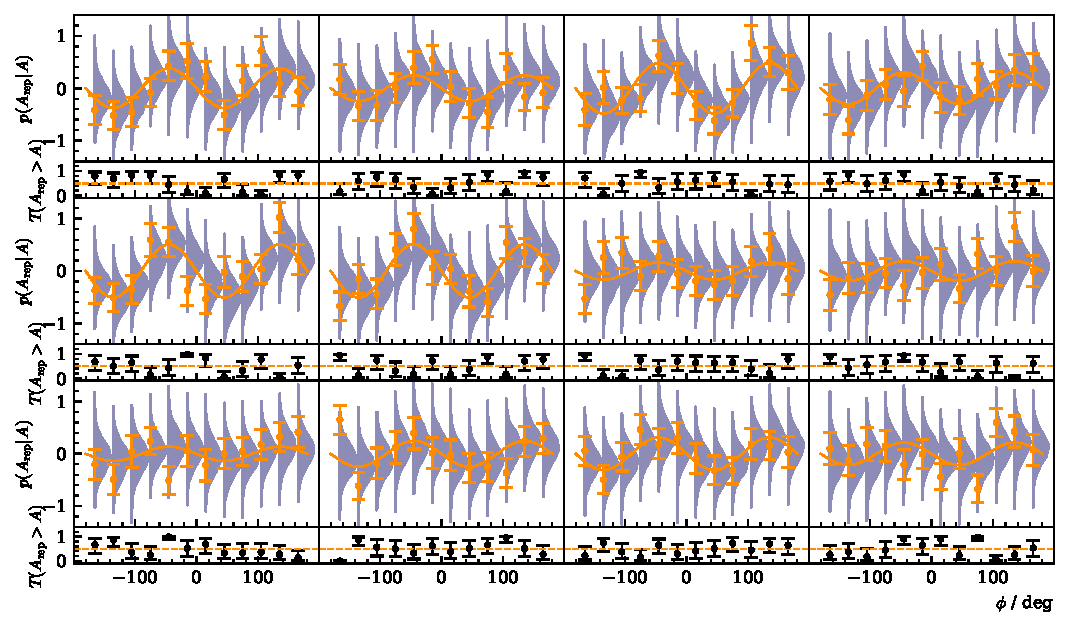
\includegraphics[width=\linewidth]{../bayes/toyMC/plots/toyMC_ppd_checks.pdf}
		\caption{Posterior predictive checks $p\left(A_\text{rep}\big|A\right)$ from a \textsc{Bayesian} fit to the event yield asymmetries for 12 toy Monte Carlo bins are shown as distributions. The data points in the upper plot are the asymmetry $A\left(\phi\right)$, which was additionally fitted using a $\chi^2$ fit (solid line). The goodness of fit is shown using $p$-values, which give the fraction $T\left(A_\text{rep}>A\right)$ of replicated samples greater than the original measured value, with propagated statistical error bars on the bottom of each plot. The expected mean value of $T\left(A_\text{rep}>A\right)=0.5$ is indicated by the dashed line. }
		\label{fig:toymc_asym}
	\end{sidewaysfigure}




\begin{figure}[htbp]
	\centering
	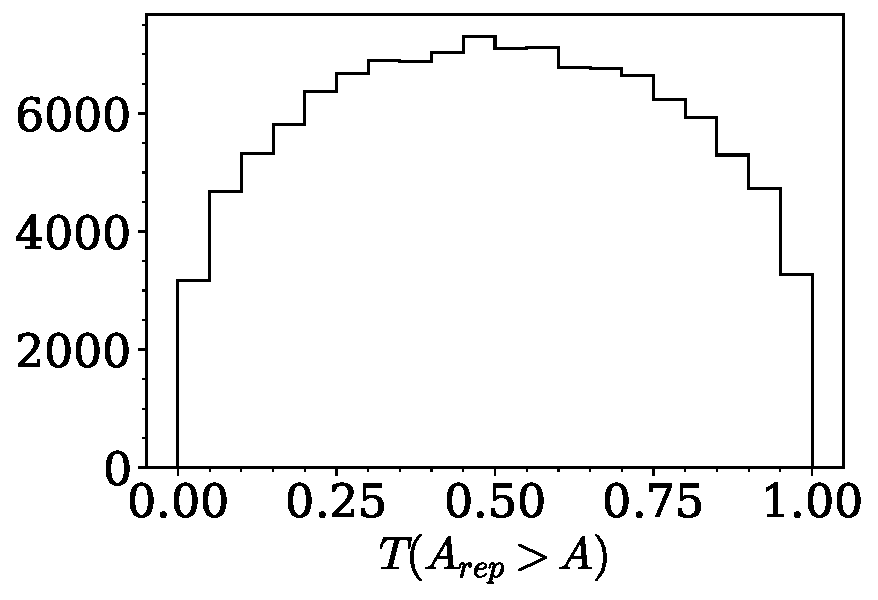
\includegraphics[width=\linewidth]{../bayes/toyMC/plots/toyMC_pval_hist.pdf}
	\caption{$p$ values of all toy Monte Carlo bins. They are centered around their mean at $0.5$, which is indicated by the dashed line, and show no bias towards higher or lower values, thus confirming an adequate fit.}
	\label{fig:toymc_pvals}
\end{figure}

\noindent To check whether the fit is unbiased and provides correct error estimation one can investigate the normalized residuals
\begin{equation}
	\xi = \frac{\Sigma^\text{fit}-\Sigma^\text{true}}{\Delta\Sigma^\text{fit}}
	\label{eq:res}
\end{equation}
 in the case of a least-squares fit. Here $\Sigma^\text{fit}$ and $\Delta\Sigma^\text{fit}$ are the value and corresponding statistical error for the beam asymmetry as obtained from the fit and $\Sigma^\text{true}$ is the true value that was used to throw the toy MC experiments. An unbiased fit with right estimation of errors yields \cite{statistics} \begin{equation}
	\xi\sim\mathcal{N}\left(0,1\right).
	\label{eq:xi}
\end{equation}
This criterion obviously cannot be applied in the same way to a \textsc{Bayesian} fit. The fit results are distributions and therefore lack point estimates $\Sigma^\text{fit}$ and errors $\Delta\Sigma^\text{fit}$. However, one can modify Equation \eqref{eq:res} to the needs of a \textsc{Bayesian} fit to assess its performance:
\begin{equation}
	\Xi=\frac{\text{median}\left(\left\{\Sigma^\text{fit}\right\}\right)-\Sigma^\text{true}}{\text{std}\left(\left\{\Sigma^\text{fit}\right\}\right)}\sim\mathcal{N}(0,1).
\end{equation}
Instead of the point estimates $\Sigma^\text{fit}$ the median of the set of all draws from the marginal posteriors $\left\{\Sigma^\text{fit}\right\}$ is shifted by the true value $\Sigma_\text{true}$ and normalized by the standard deviation as an error estimate for each fit. Although this is not a rigorously derived quantity it allows to identify possible bias if $\text{mean}\left(\Xi\right)\neq 0$. Furthermore, checking that $\sigma\approx1$ will affirm whether the width of the marginal posterior distributions is sensible. Figure \ref{fig:toymcpost} shows the combined $\Xi$-distributions of all fits and the unaltered combined posteriors shifted by the true value. As expected, both distributions are normal as a \textsc{Gaussian} fit proves.  
\begin{figure}[htbp]
	\centering
	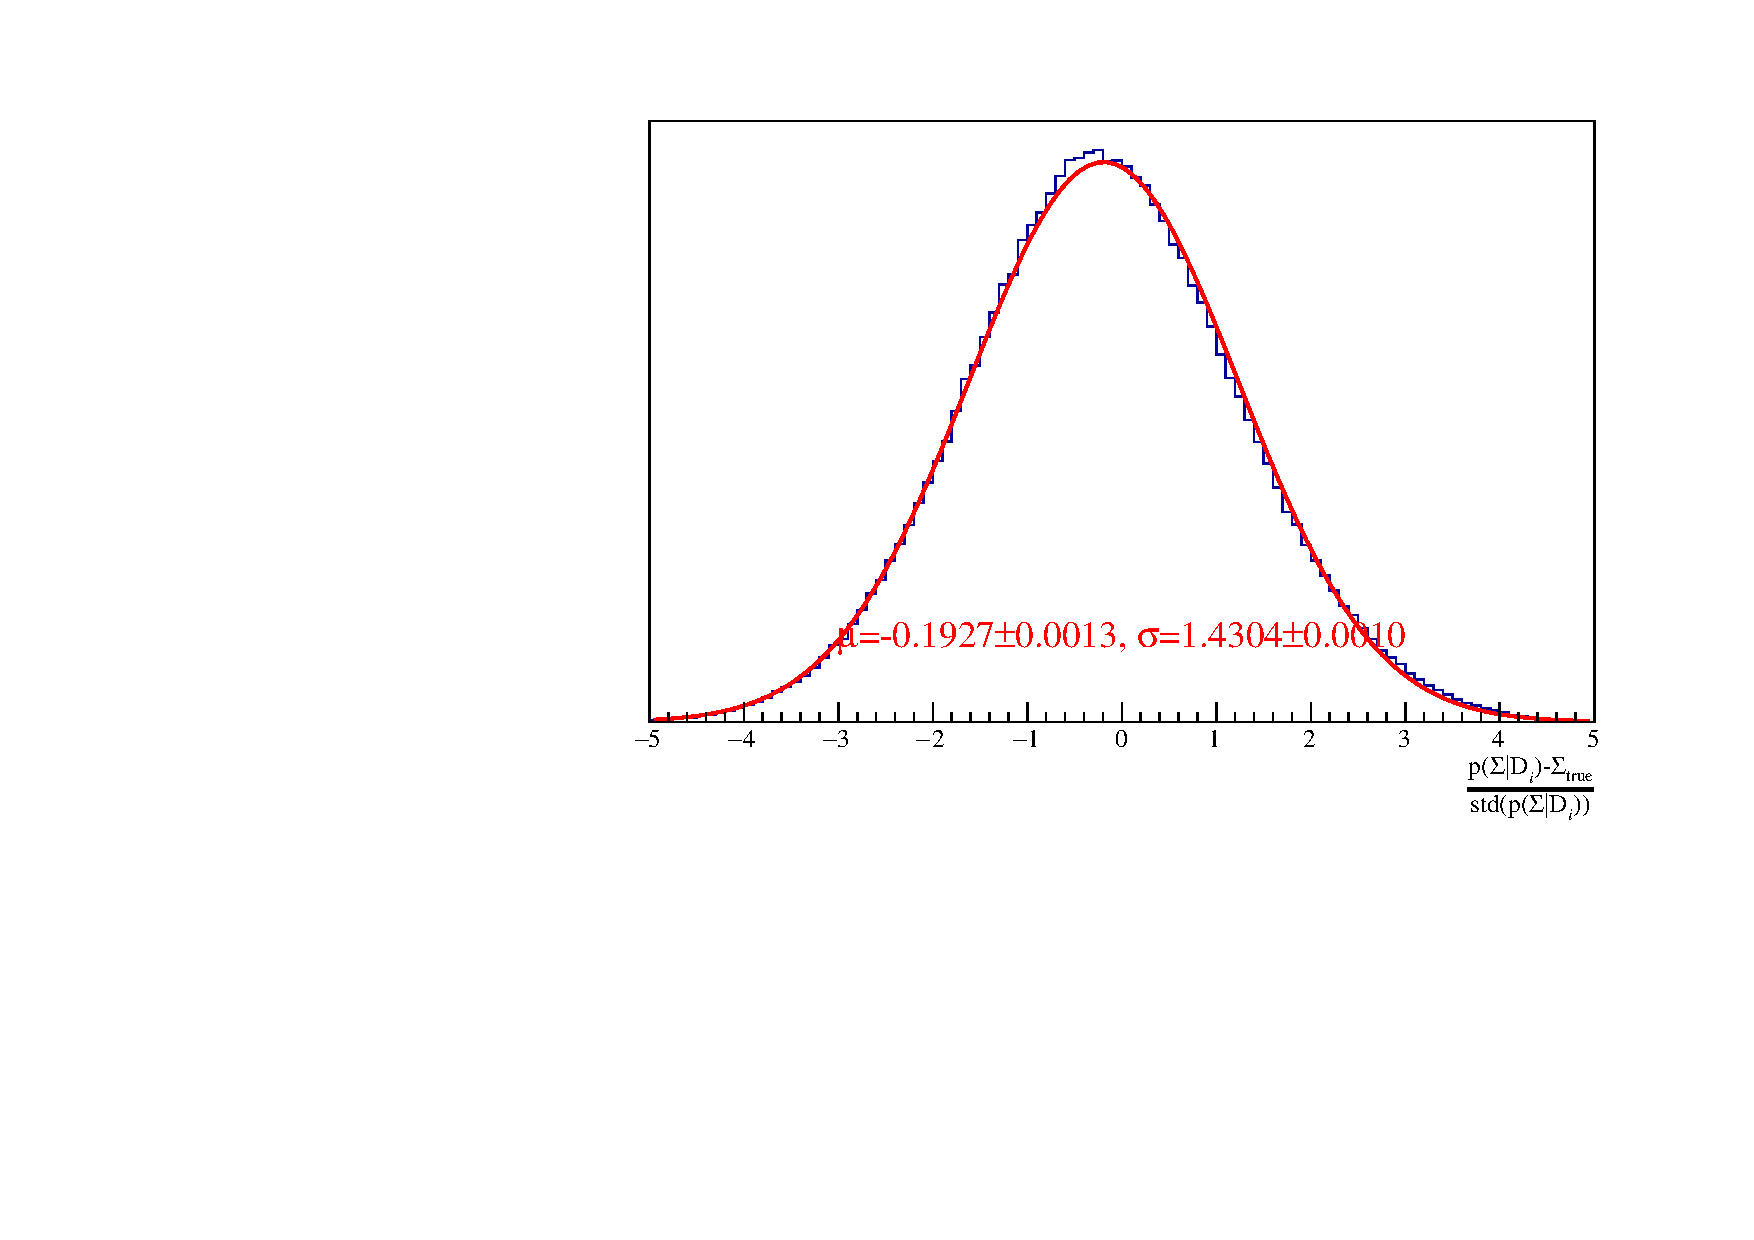
\includegraphics[width=.49\linewidth]{../bayes/toyMC/plots/combined_post_add.pdf}
	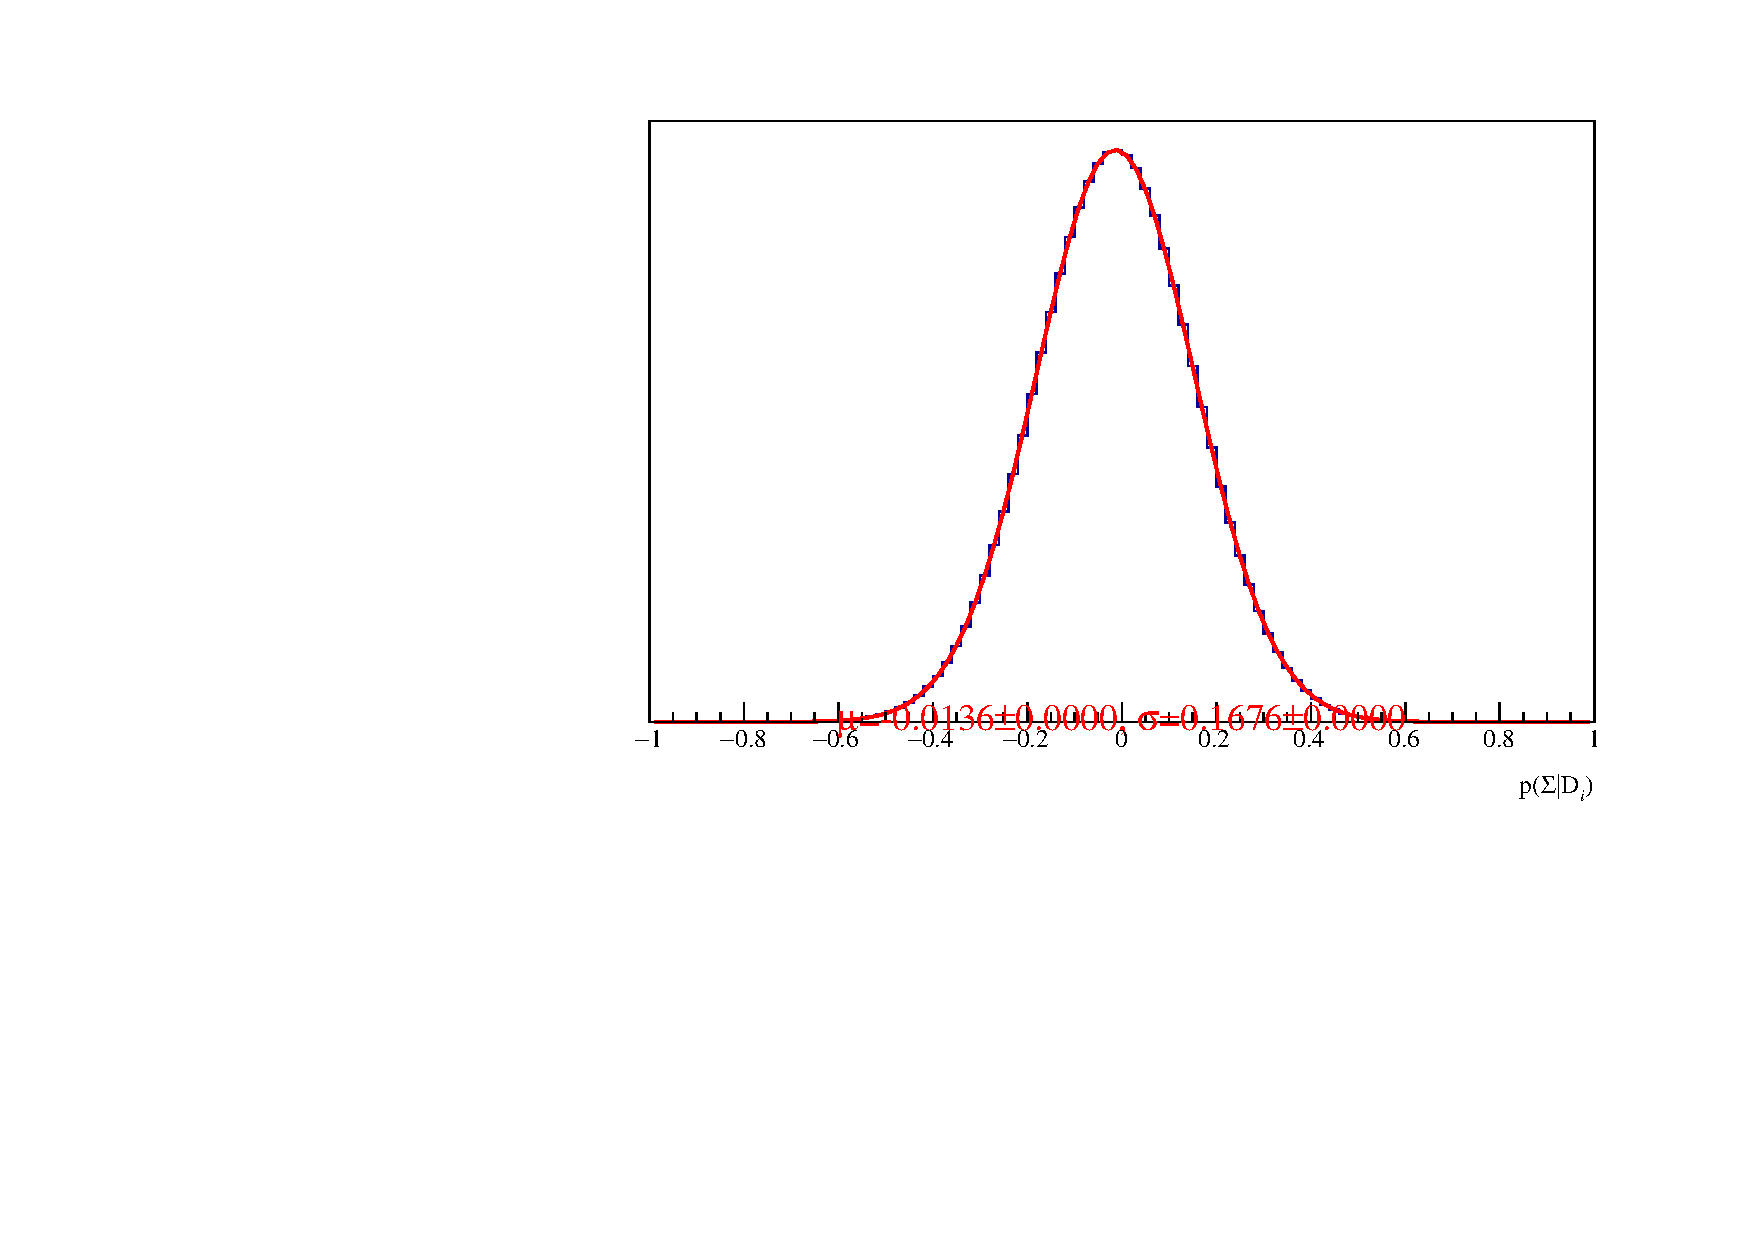
\includegraphics[width=.49\linewidth]{../bayes/toyMC/plots/combined_post_add_raw.pdf}
	\caption{Left: Combined posterior distributions of all $10000$ fits normalized by their respective standard deviation. Right: Unaltered combined posterior distributions of all $10000$ fits. A \textsc{Gaussian} fit was performed to determine mean $\mu$ and standard deviation $\sigma$ of the distributions with results given on top.}
	\label{fig:toymcpost}
\end{figure}
The width of the marginal posterior distributions can be regarded as sensible since the standard deviation of the $\Xi$ distribution $\sigma_\Xi\approx1$\footnote{One cannot expect to fulfill Eq. \eqref{eq:xi} exactly, since the errors are after all only estimates that aim to create comparability to the least squares fit.}. This is furthermore confirmed by the fact that $\left\{\Sigma^\text{fit}\right\}-\Sigma^\text{true}=0$ within one standard deviation of the \textsc{Gaussian}. Yet, the fit results tend to underestimate the beam asymmetry, because both distributions are centered out of their statistical error at $\mu\pm\Delta\mu<0$. This indicates bias towards smaller values of the beam asymmetry. Remarkably, this bias is \emph{not} introduced by the \textsc{Bayesian} fit, but by the choice of binning and available statistics as an extensive investigation of binned fits (least squares and \textsc{Bayesian}) to toy Monte Carlo data showed. A detailed discussion thereof is given in appendix \ref{app:binnedfits}. For now it suffices to note the origin of this bias lies in the choice of binning and is thus inevitable. And, most importantly, the introduced bias is negligible compared to the width of the posterior distributions, so that a binned fit will produce valid fit results in any case. Nevertheless this emphasizes the advantage of unbinned fitting, which is discussed in the next paragraph.

It has been established that the fit produces valid results with sensible statistical errors, i.e. widths of posterior distributions, and the description of the data is in agreement with the expectations. It remains to diagnose the convergence of the \textsc{Markov} chains to finally deem the binned fit method appropriate. For this the $\widehat{R}$ value and the relative Monte Carlo standard error (MCSE) $\frac{\sigma_\text{MCSE}}{\text{median}\left[p\left(\Sigma|y\right)\right]}$ that were introduced in section \ref{sec:bayes} are investigated. If $\widehat{R}<1.05$ one can assume that the different chains have converged and explored the same parameter space \cite{rhat}. Furthermore the accuracy supplied by the number of draws from the posteriors can be evaluated with the relative MCSE. It is demanded that $\frac{\sigma_\text{MCSE}}{\text{median}\left[p\left(\Sigma|y\right)\right]}\lesssim 5\%$. This is the case for $97\%$ of all fits, see Figure \ref{fig:toyMC_diagnostics} on the left. When the fit result for the beam asymmetry is close to $0$ larger values for the relative MCSE are observed. The $\widehat{R}$ values (Figure \ref{fig:toyMC_diagnostics} on the right) clearly indicate good within and between chain convergence. This means that the hyper parameters $n_\text{chain},n_\text{samples}$ and $n_\text{warm up}$ as chosen are well tuned, although one may increase the number of sample draws from the posterior for the fit from measured data to further suppress the relative MCSE. Then, only $11\cdot12$  as opposed to $10000$ fits have to be performed keeping the computational cost reasonable.    
\begin{figure}[htbp]
	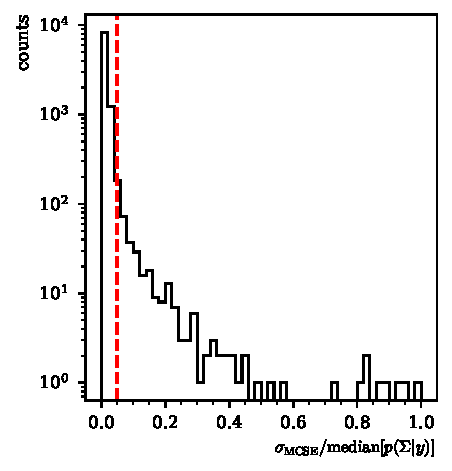
\includegraphics[width=.49\linewidth]{../bayes/toyMC/plots/toyMC_mcse_hist.pdf}
	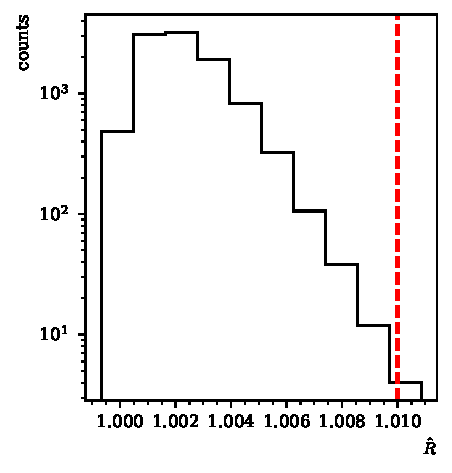
\includegraphics[width=.49\linewidth]{../bayes/toyMC/plots/toyMC_rhat_hist.pdf}
	\caption{ Left: relative error $\frac{\sigma_\text{MCSE}}{\text{median}\left[p\left(\Sigma|y\right)\right]}$ Right: $\widehat{R}$ associated with the fit parameter $\Sigma$. Both are shown for all 10000 fits. The critical values that should not be exceeded are marked by dashed lines.}
	\label{fig:toyMC_diagnostics}
\end{figure}
\subsubsection{Event based fit}
Not only signal events but also contributions from random time background as well as the imperfect detector efficiency $\epsilon(\phi)$ have to be simulated in order to test the method of event based fitting. For each polarization setting prompt peak and sideband events are drawn from the theoretical $\phi$-distributions $p_\text{prompt}$ and $p_\text{sideband}$ which are given in Equations \eqref{eq:pprmpt} and \eqref{eq:pside}. The total number of draws per setting and bin is again given by \textsc{Poisson} distributions and the ratio of prompt peak to sideband events is given by the time cut weights $\left\{w_i\right\}_{i=1}^7$ employed for the actual analysis of the $p\eta$ final state data \cite{farahphd}. This means that seven times prompt peak and sideband events need to be simulated. The fraction of signal events within the prompt peak $f$ was set to $f=0.95$. Further, the values $p_\gamma^\parallel=0.25,p_\gamma^\bot=0.3,\Sigma=0.5$, $\Sigma^\text{bkg}=-0.5$ and lastly, a random efficiency function as already chosen in reference \cite{farahphd} were appointed. Finally the hyperparameters $n_\text{chain},n_\text{samples},n_\text{warm up}$ are chosen in the same way as previously described. Table \ref{tab:mcsum} shows a summary of all toy Monte Carlo properties.
\begin{table}[htbp]

	\renewcommand{\arraystretch}{1.5}
	\centering
	\begin{tabularx}{\linewidth}{l|XXX}
		\toprule
		\textbf{chosen parameters} & \multicolumn{3}{l}{$p_\gamma^\parallel=0.25,p_\gamma^\bot=0.3,\Sigma=0.5$, $\Sigma^\text{bkg}=-0.5$, $f=0.95$,}\\ &\multicolumn{3}{l}{$w_1=\frac{15}{210},w_2=\frac{8}{210},w_3=\frac{4}{210},w_4=\frac{10}{210},w_5=\frac{14}{210},w_6=\frac{6}{210},w_7=\frac{11}{210}$}\\
		\hline
		\textbf{simulation draws} &\multicolumn{3}{c}{$7\cdot N^\parallel_{\text{total},i}\sim\mathcal{P}(800)$, $7\cdot N^\bot_{\text{total},i}\sim\mathcal{P}(1000)\quad\big|_{i=1}^7$}\\
		\cline{2-4}
		&signal in prompt&background in prompt& sideband \\
		&$N^{\parallel/\bot}_\text{total}\cdot f$&$N^{\parallel/\bot}_\text{total}\cdot\left(1-f\right)$&$N^{\parallel/\bot}_\text{total}\cdot\left(1-f\right)\cdot1/w_i$\\
		\hline
		\textbf{efficiency function}&\multicolumn{3}{l}{$\epsilon\left(\phi\right)=1/10.5\cdot\left(9.3+0.28\cdot\cos\phi+0.24\cdot\sin3\phi\right)$}\\
		\hline
		\textbf{hyperparameters}&\multicolumn{3}{l}{$n_\text{samples}=1000,n_\text{chain}=4,n_\text{warm up}=1000$}\\
		\bottomrule
	\end{tabularx}
	\caption{Summary of the complete setting of all toy Monte Carlo experiments for the event based fit. Values and table layout adapted from \cite{farahphd}.}
	\label{tab:mcsum}
\end{table}
In total, 1000\footnote{The computation time for 10000 toy Monte Carlo fits would have exceeded a full week.} toy Monte Carlo experiments are thrown. To evaluate the fit results only the posterior distributions are available. As before, the residuals $\Xi$ are built from all fits, now for $\Sigma$ as well as $\Sigma^\text{bkg}$. They are shown in Figure \ref{fig:toyMCposteriors} together with the unnormalized posterior distributions. 
\begin{figure}[htbp]
	\centering
	\begin{subfigure}{\linewidth}
		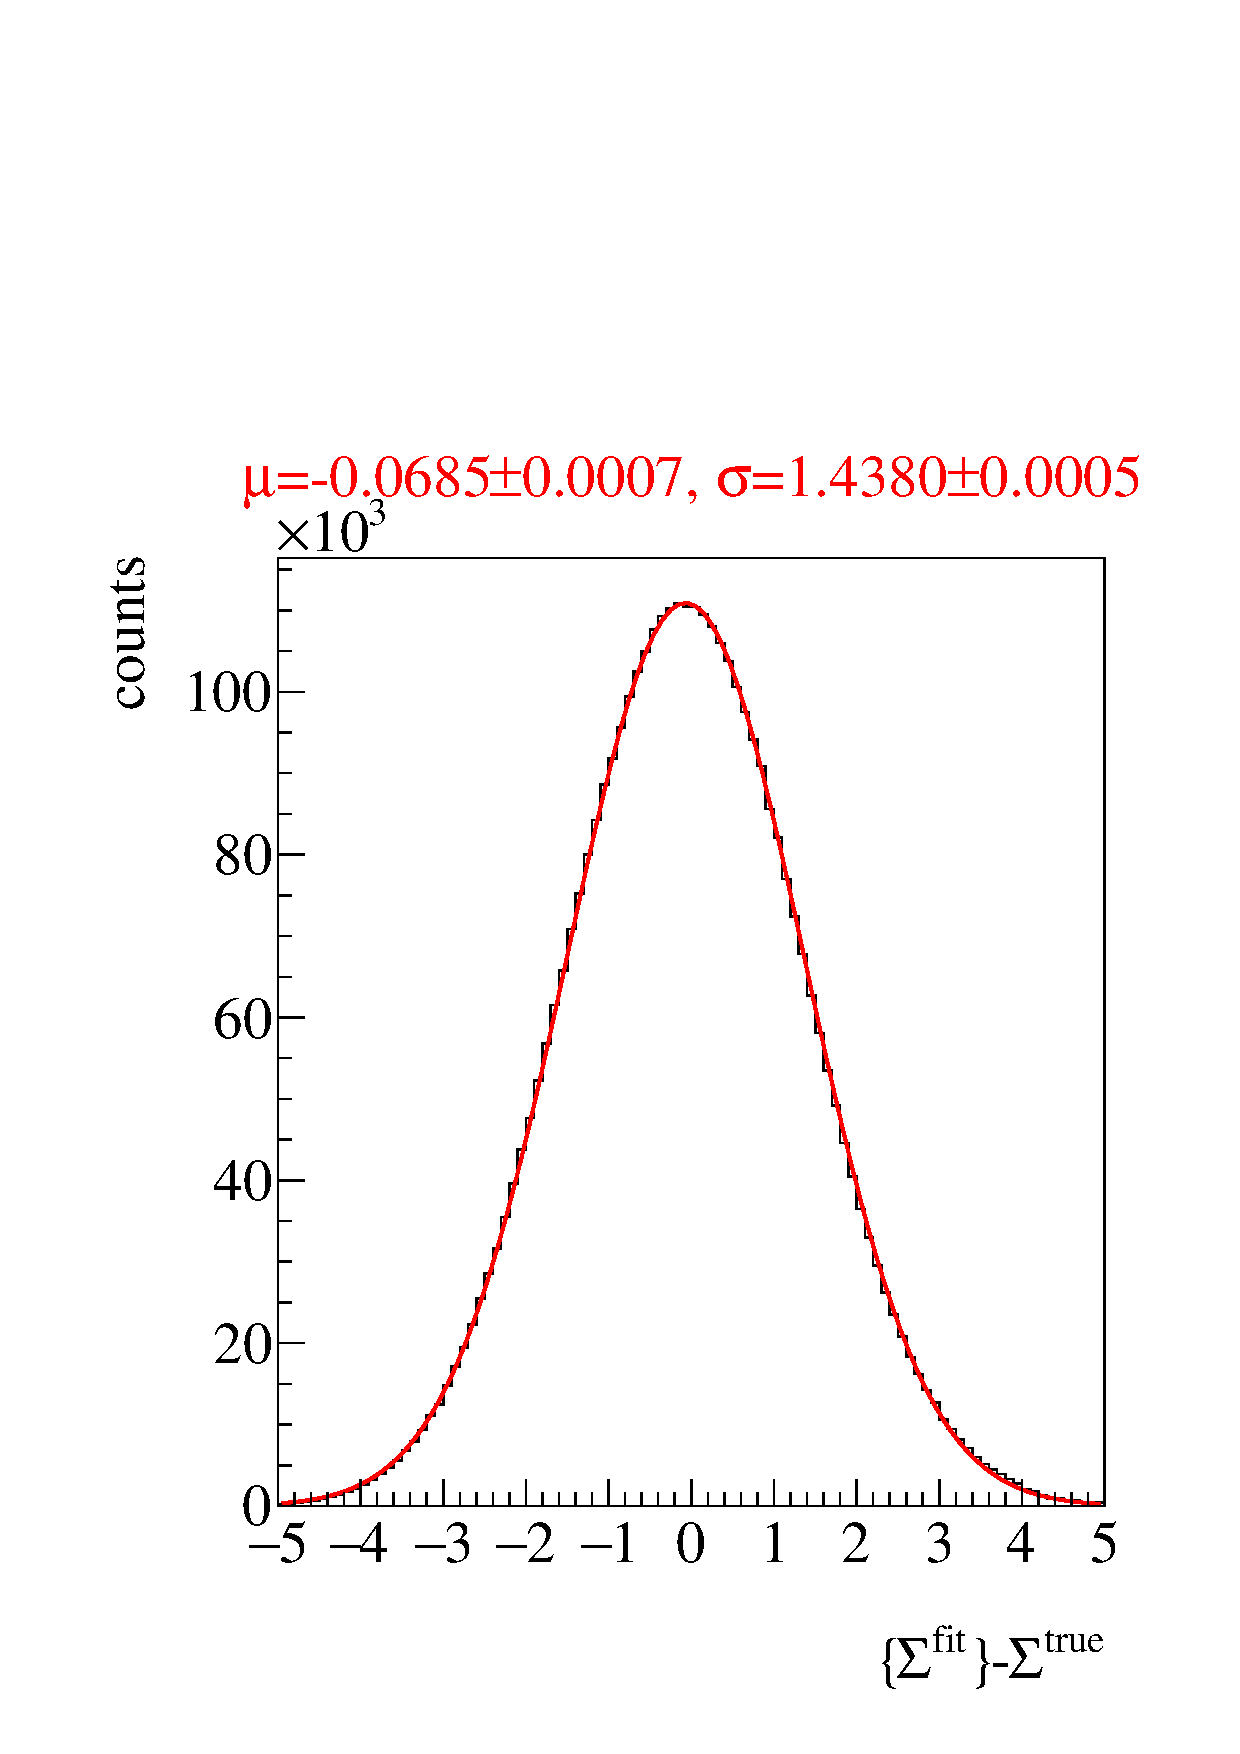
\includegraphics[width=.49\linewidth]{../bayes/event_based_fit/plots/combined_post_add.pdf}
		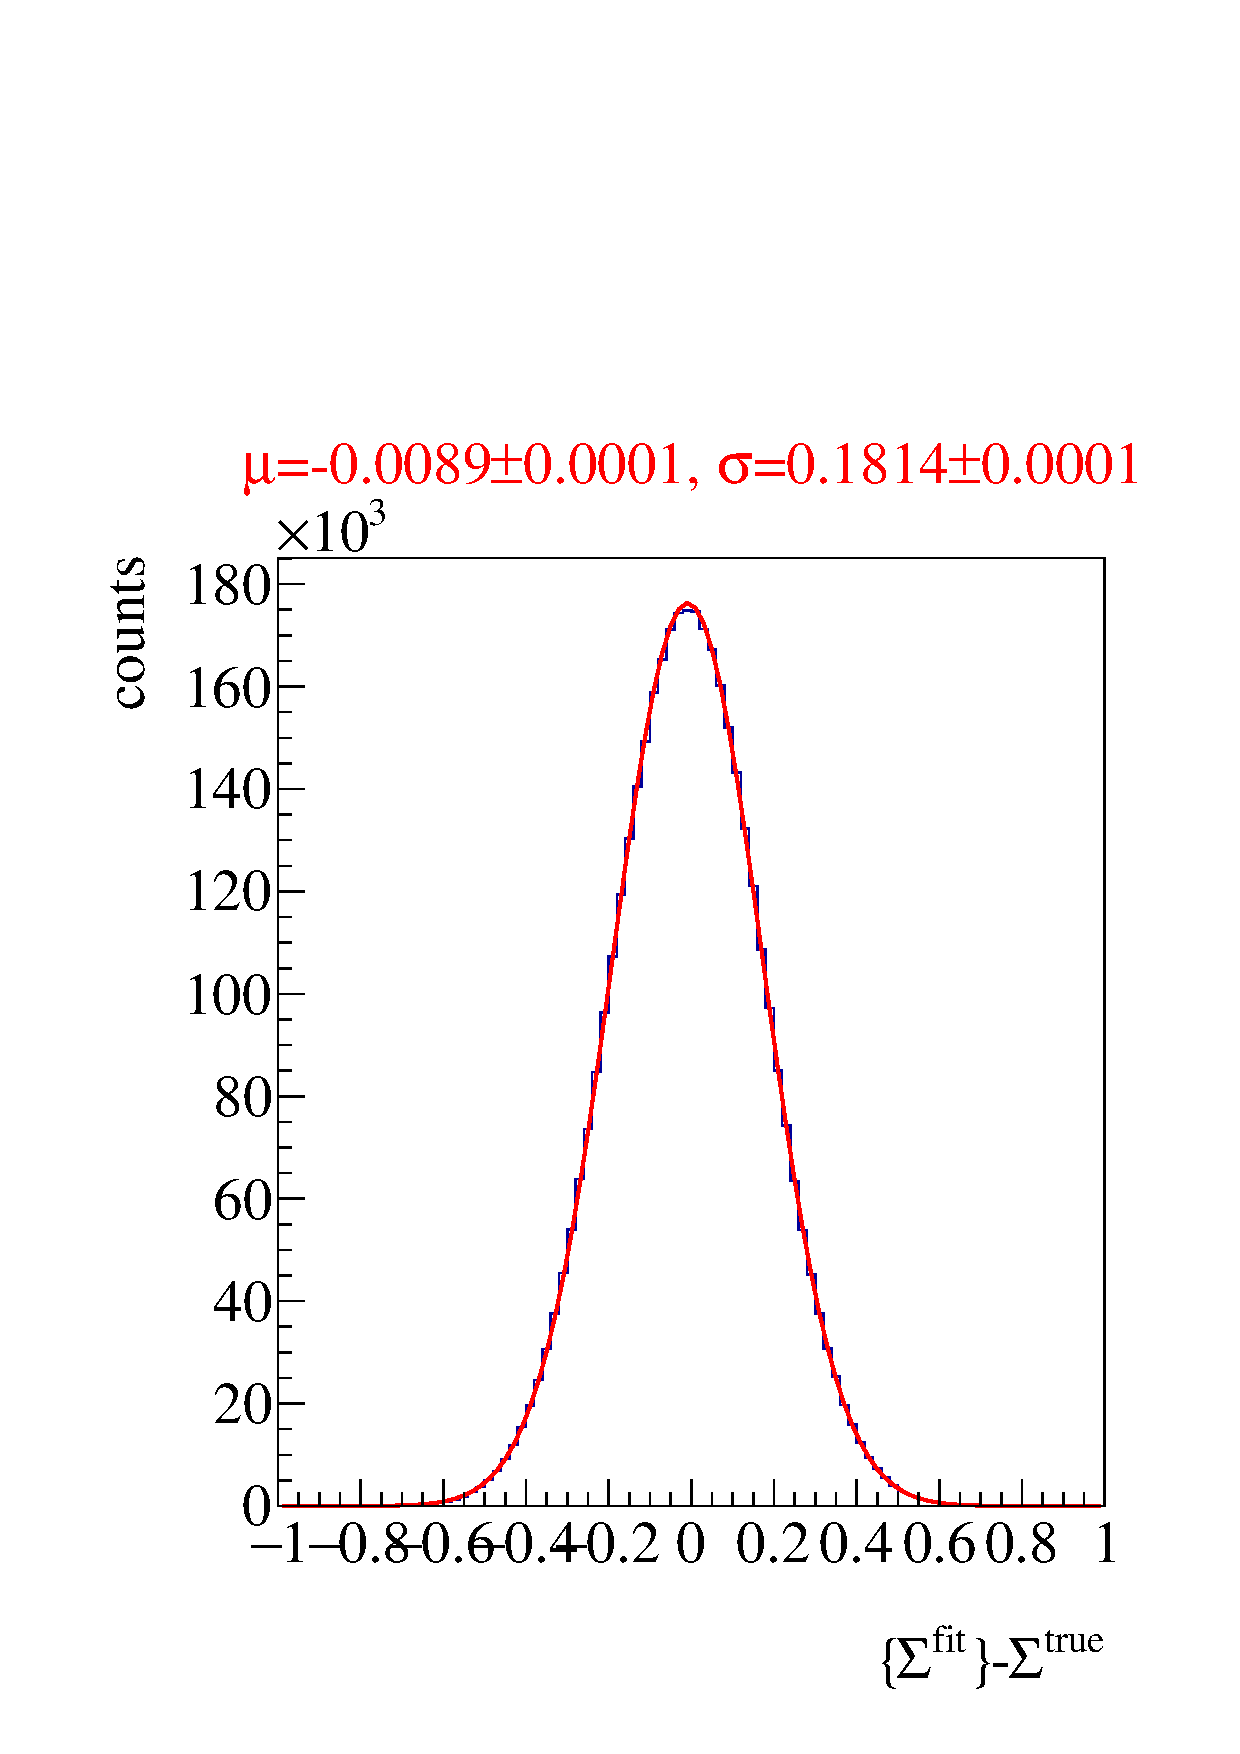
\includegraphics[width=.49\linewidth]{../bayes/event_based_fit/plots/combined_post_add_raw.pdf}
		\subcaption{Signal beam asymmetry $\Sigma$}
	\end{subfigure}
	\begin{subfigure}{\linewidth}
		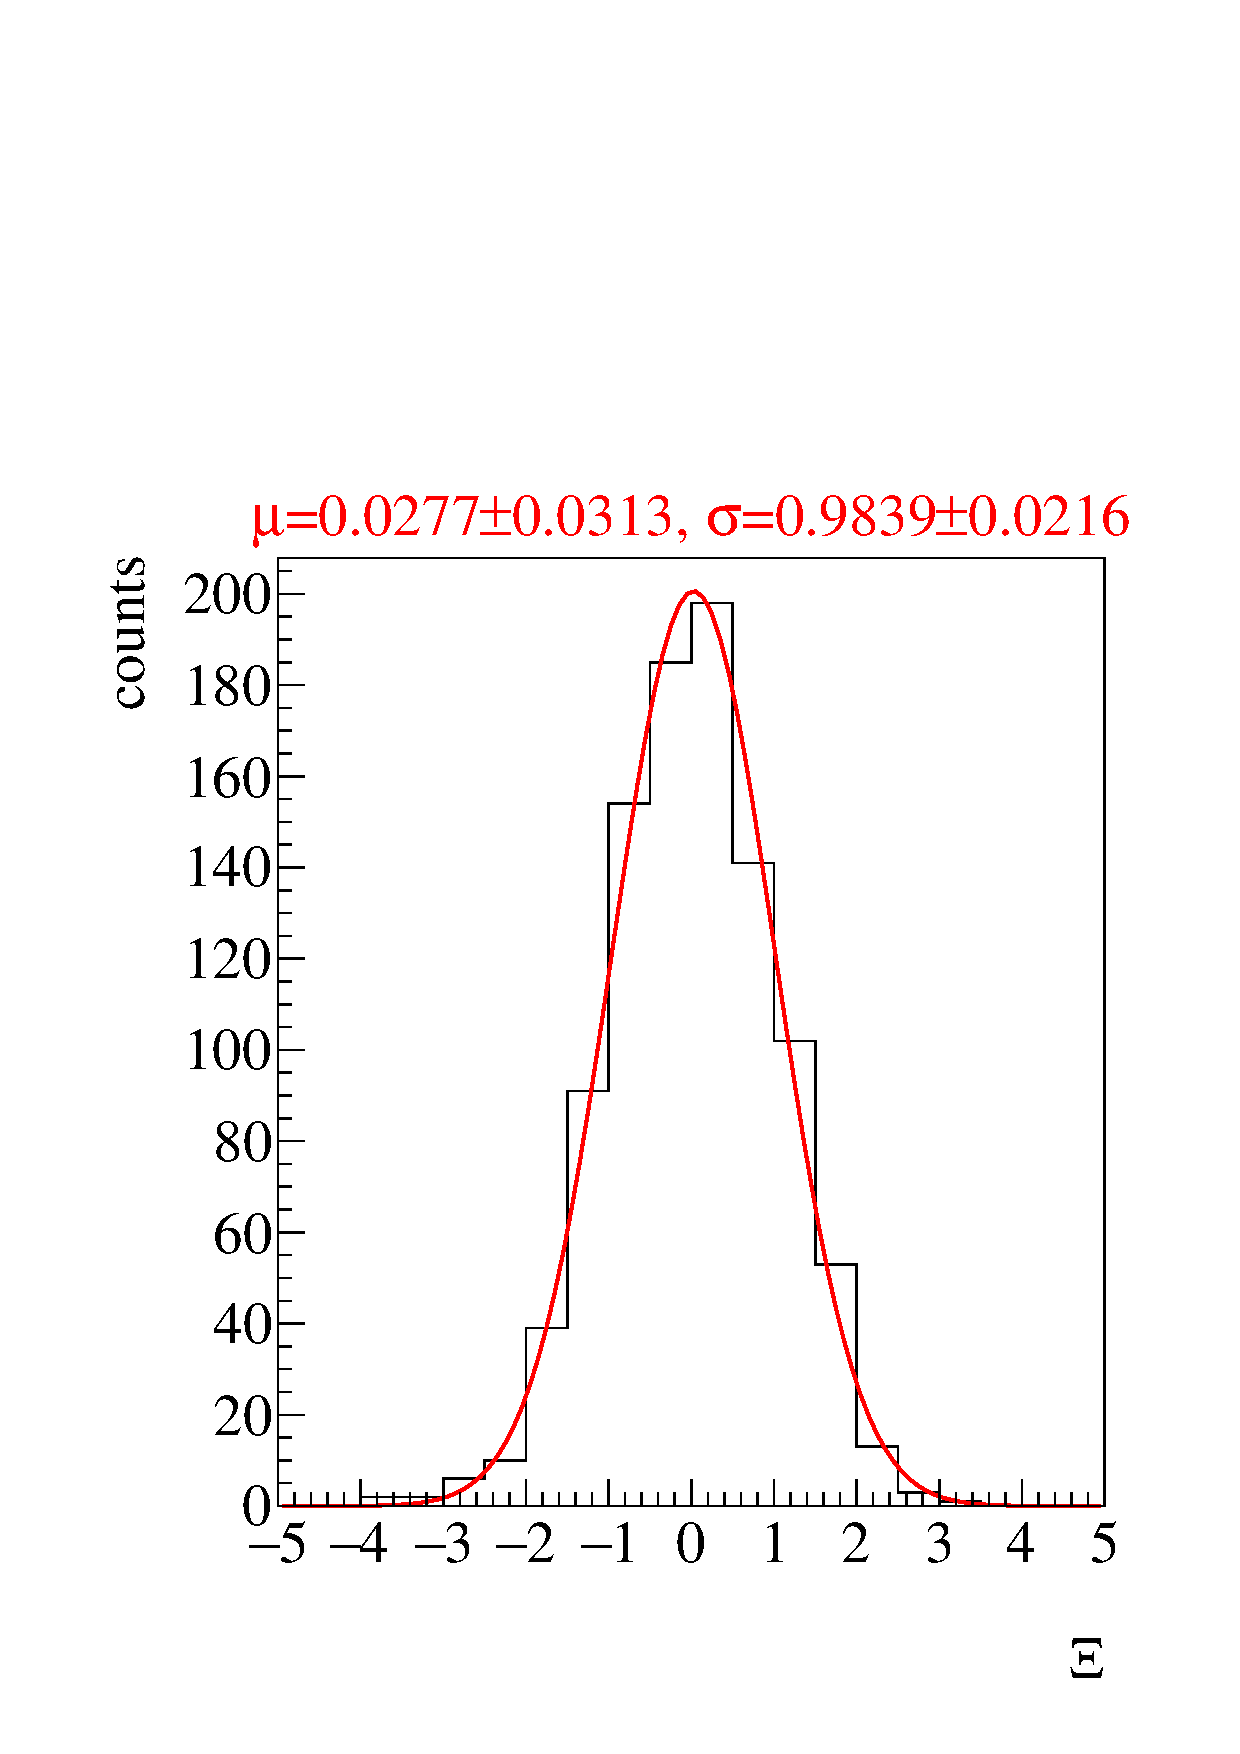
\includegraphics[width=.49\linewidth]{../bayes/event_based_fit/plots/combined_post_add_bkg.pdf}
		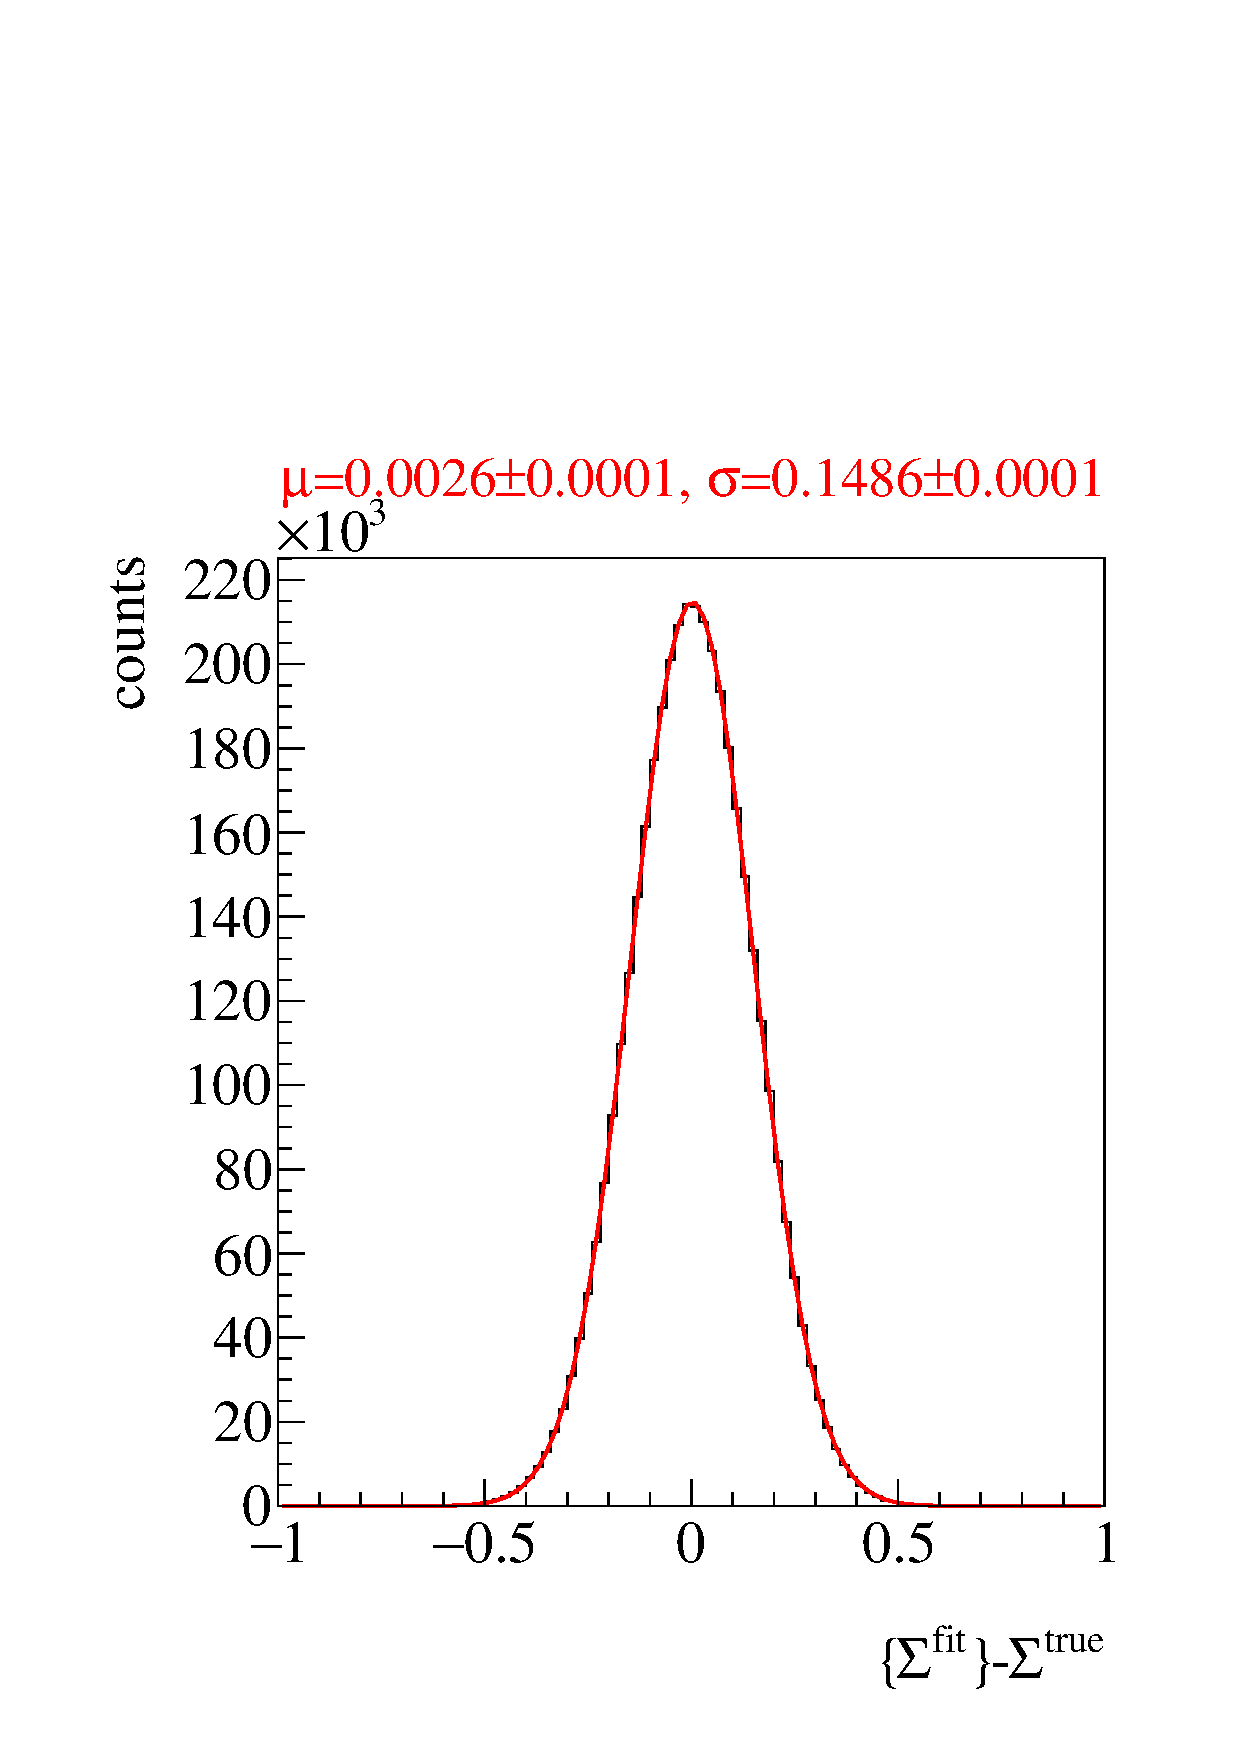
\includegraphics[width=.49\linewidth]{../bayes/event_based_fit/plots/combined_post_add_raw_bkg.pdf}
		\subcaption{Background beam asymmetry $\Sigma^\text{bkg}$}
	\end{subfigure}
	\caption{Combined posteriors for the beam asymmetries $\Sigma$ and $\Sigma^\text{bkg}$ from all 1000 event based fits. Left: Residuals $\Xi$ Right: Unnormalized posterior distributions. A \textsc{Gaussian} fit is performed on the distributions with results for mean $\mu$ and standard deviation $\sigma$ on top.}
	\label{fig:toyMCposteriors}
\end{figure}
Note that the distributions are truncated towards the tails at $\Sigma\to1$ and $\Sigma^\text{bkg}\to-1$ as implemented in the \textsc{Bayesian} fit in Stan. Also the event based fit is able to reproduce the true values within one standard deviation of the posterior distribution $\sigma_\text{posterior}$. Only slight bias towards smaller values of the signal beam asymmetry is seen, but again with negligible effect on the results in comparison to the widths of the distributions. Additionally, the mean of the distributions are 0 within $3\sigma$ of their statistical error and the errors are estimated correctly, since $\sigma_\text{posterior}=1$ within the statistical error. Note that the background beam asymmetry is estimated closer to its true value than the signal beam asymmetry because there are more random background events than signal events.

If the total amount of posterior distributions is not too large one might also combine them in a \emph{pooled likelihood} approach (see subsection \ref{subsec:combinf}). This is shown in Figure \ref{fig:poollik} for both determined asymmetries.
\begin{figure}[htbp]
	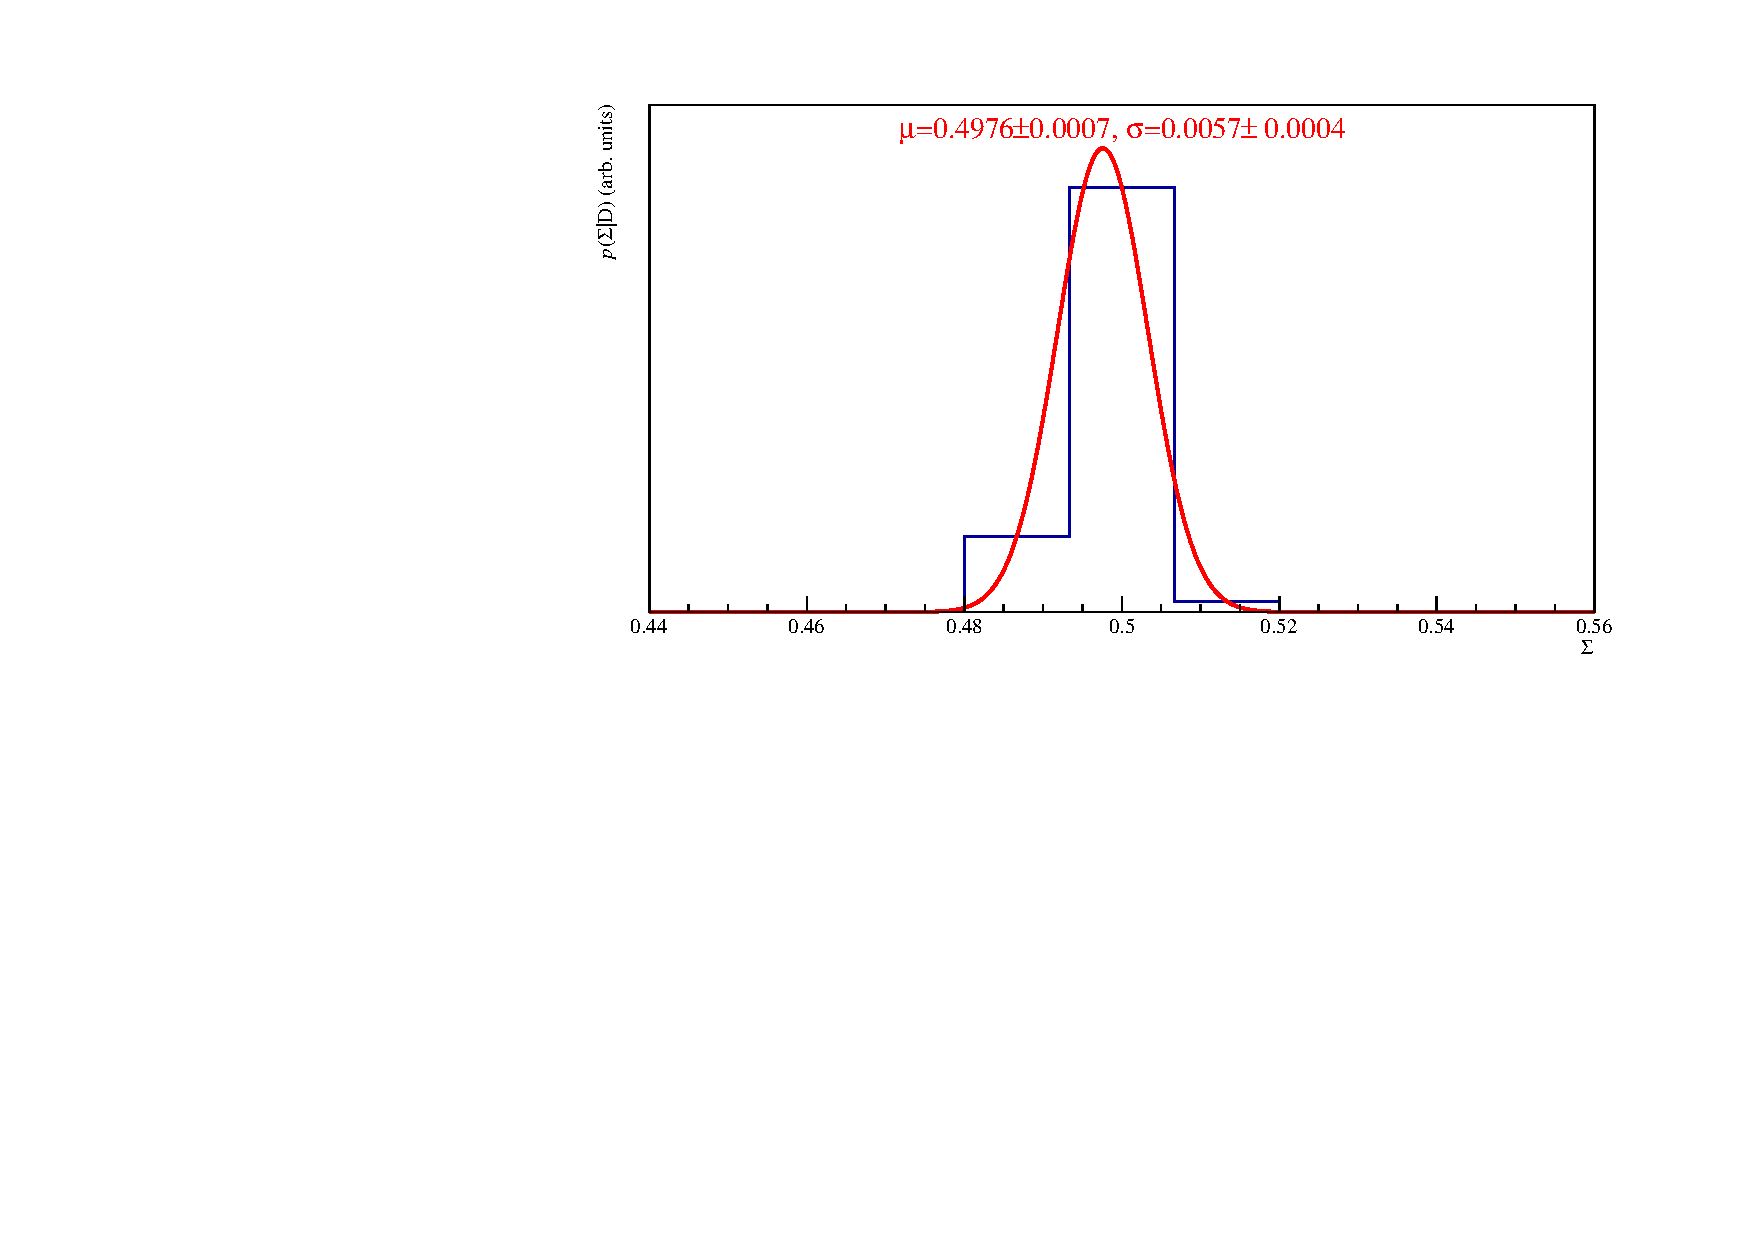
\includegraphics[width=.49\linewidth]{../bayes/event_based_fit/plots/combined_post_mul.pdf}
	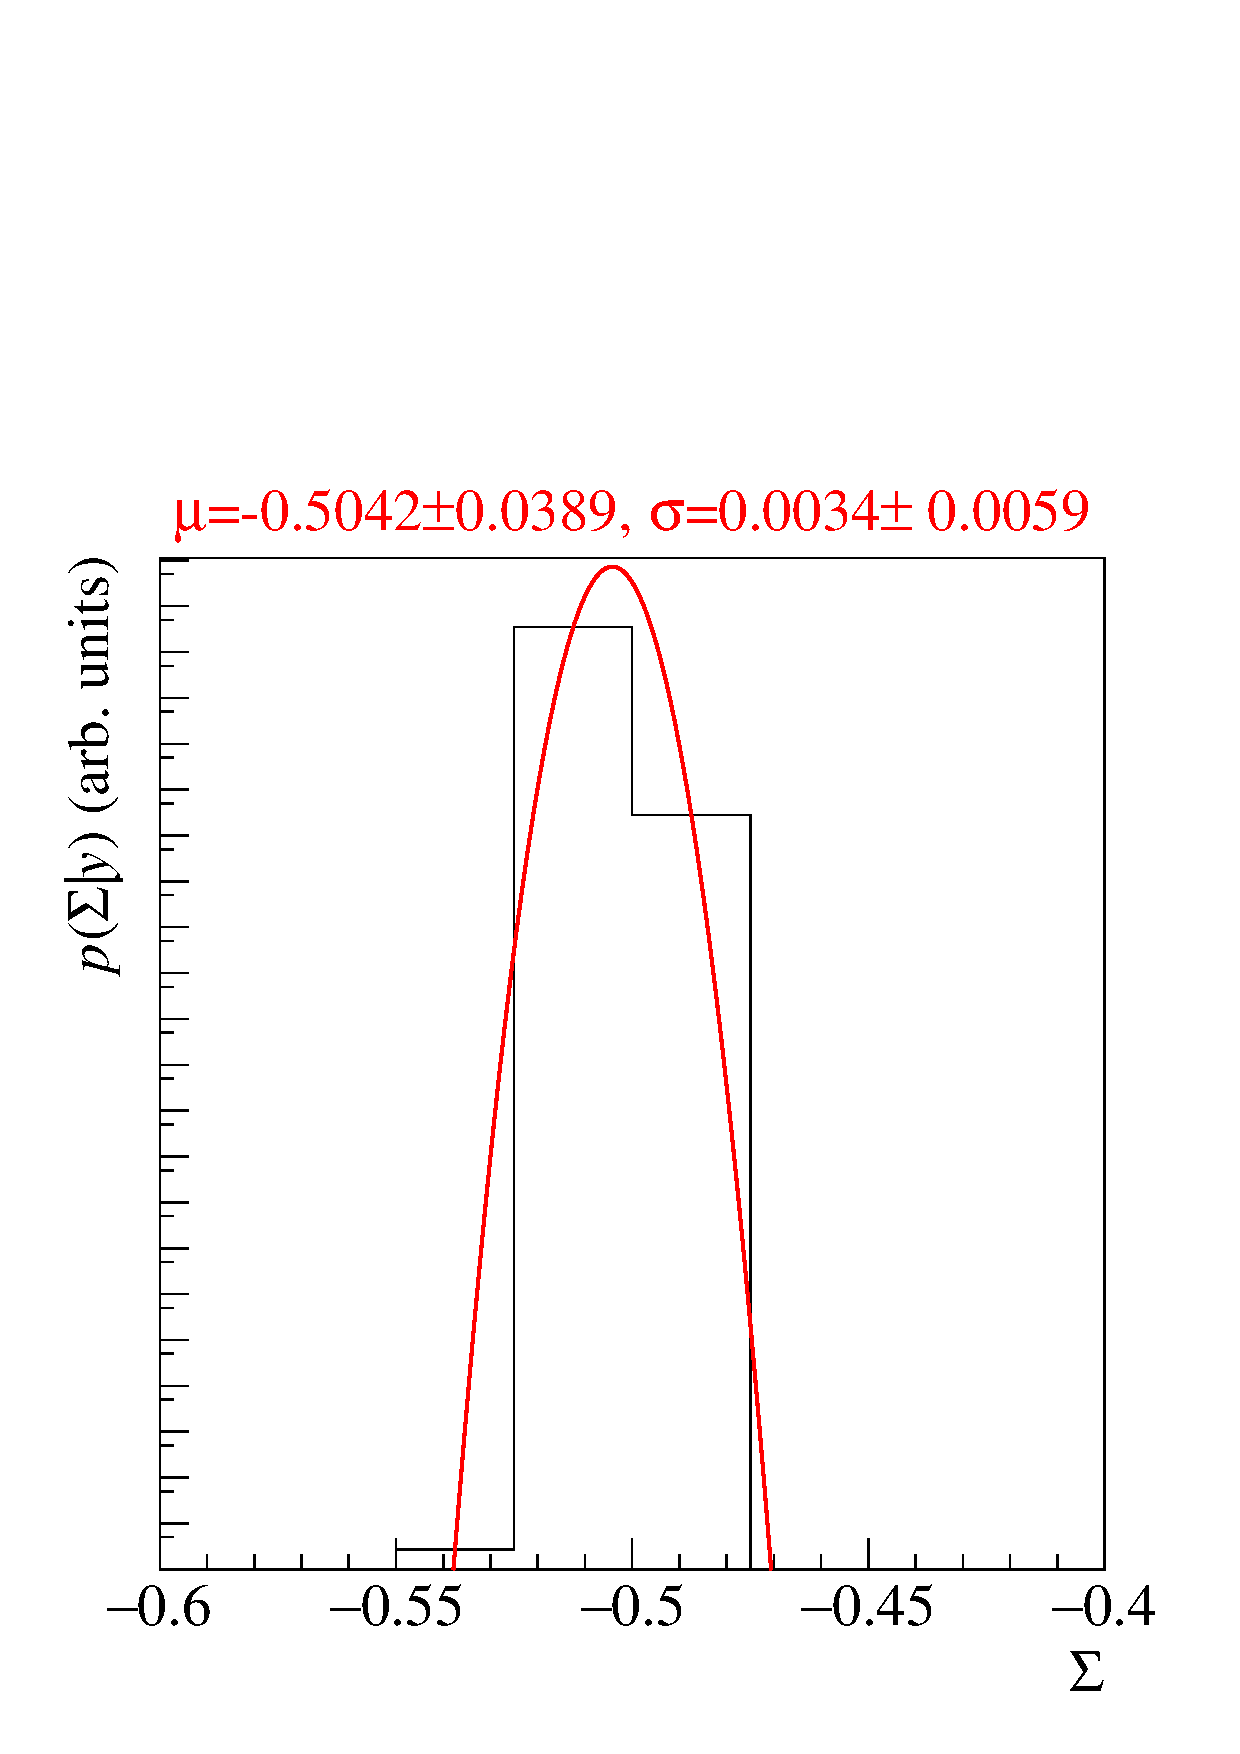
\includegraphics[width=.49\linewidth]{../bayes/event_based_fit/plots/combined_post_mul_bkg.pdf}
	\caption{Combined posterior probabilities using the \emph{pooled likelihood} approach. Left: Signal beam asymmetry, Right: background beam asymmetry. Mean and standard deviation as obtained from a \text{Gaussian} fit are shown on top}
	\label{fig:poollik}
\end{figure}
 Because the true asymmetries are within $1\sigma$ of the resulting distribution one can finally conclude that the event based fit estimates positions and widths of the posterior distributions correctly. 
 
 A check of the relative MCSE and $\widehat{R}$ values as shown in Figure \ref{fig:toyMC_diagnostics1} reveals also that the hyperparameters $n_\text{chain},n_\text{samples},n_\text{warm up}$ are correctly tuned.
 \begin{figure}[htbp]
 	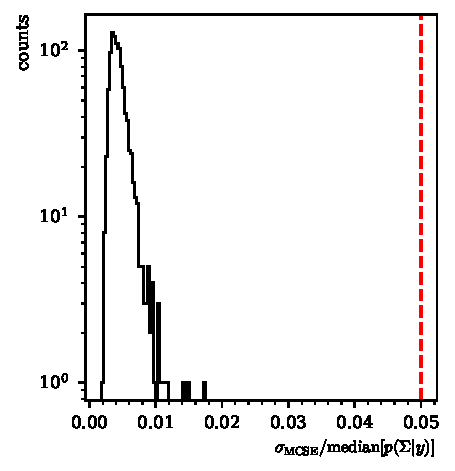
\includegraphics[width=.49\linewidth]{../bayes/event_based_fit/plots/toyMC_mcse_hist.pdf}
 	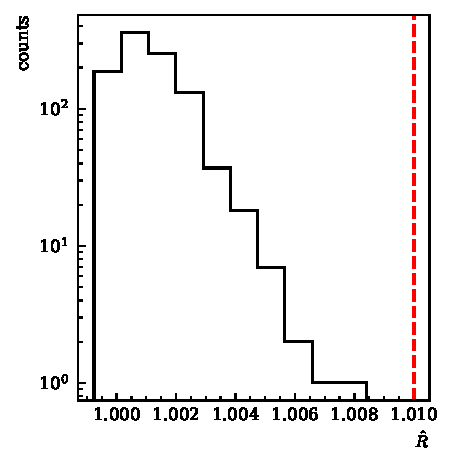
\includegraphics[width=.49\linewidth]{../bayes/event_based_fit/plots/toyMC_rhat_hist.pdf}
 	\caption{ Left: relative error $\frac{\sigma_\text{MCSE}}{\text{median}\left[p\left(\Sigma|y\right)\right]}$ Right: $\widehat{R}$ associated with the fit parameter $\Sigma$. Both are shown for all 1000 fits. The critical values that should not be exceeded are marked by dashed lines.}
 	\label{fig:toyMC_diagnostics1}
 \end{figure}
It is noteworthy that the event based fit creates more precise results regarding the MCSE although less Monte Carlo experiments in total were performed than for the binned fit. 

Next to signal and background beam asymmetry the fit also estimates an efficiency function $\epsilon(\phi)$ that is described by a \textsc{Fourier} series. The polarization weighted sum of event yields allows to confirm whether a good description of the efficiency is achieved because it is given by the efficiency function modulated only by a constant, see previous section \ref{sec:meth} $\alpha \tilde{N}^\parallel + \beta\tilde{N}^\bot = c\cdot\epsilon\left(\phi\right).$ Figure \ref{fig:toyMC_eff_func} shows the weighted sum of event yields with the same binning as used in the binned fit together with a posterior predictive check using the draws of all parameters distributions $a,b$. 
\begin{figure}[htbp]
	\centering
	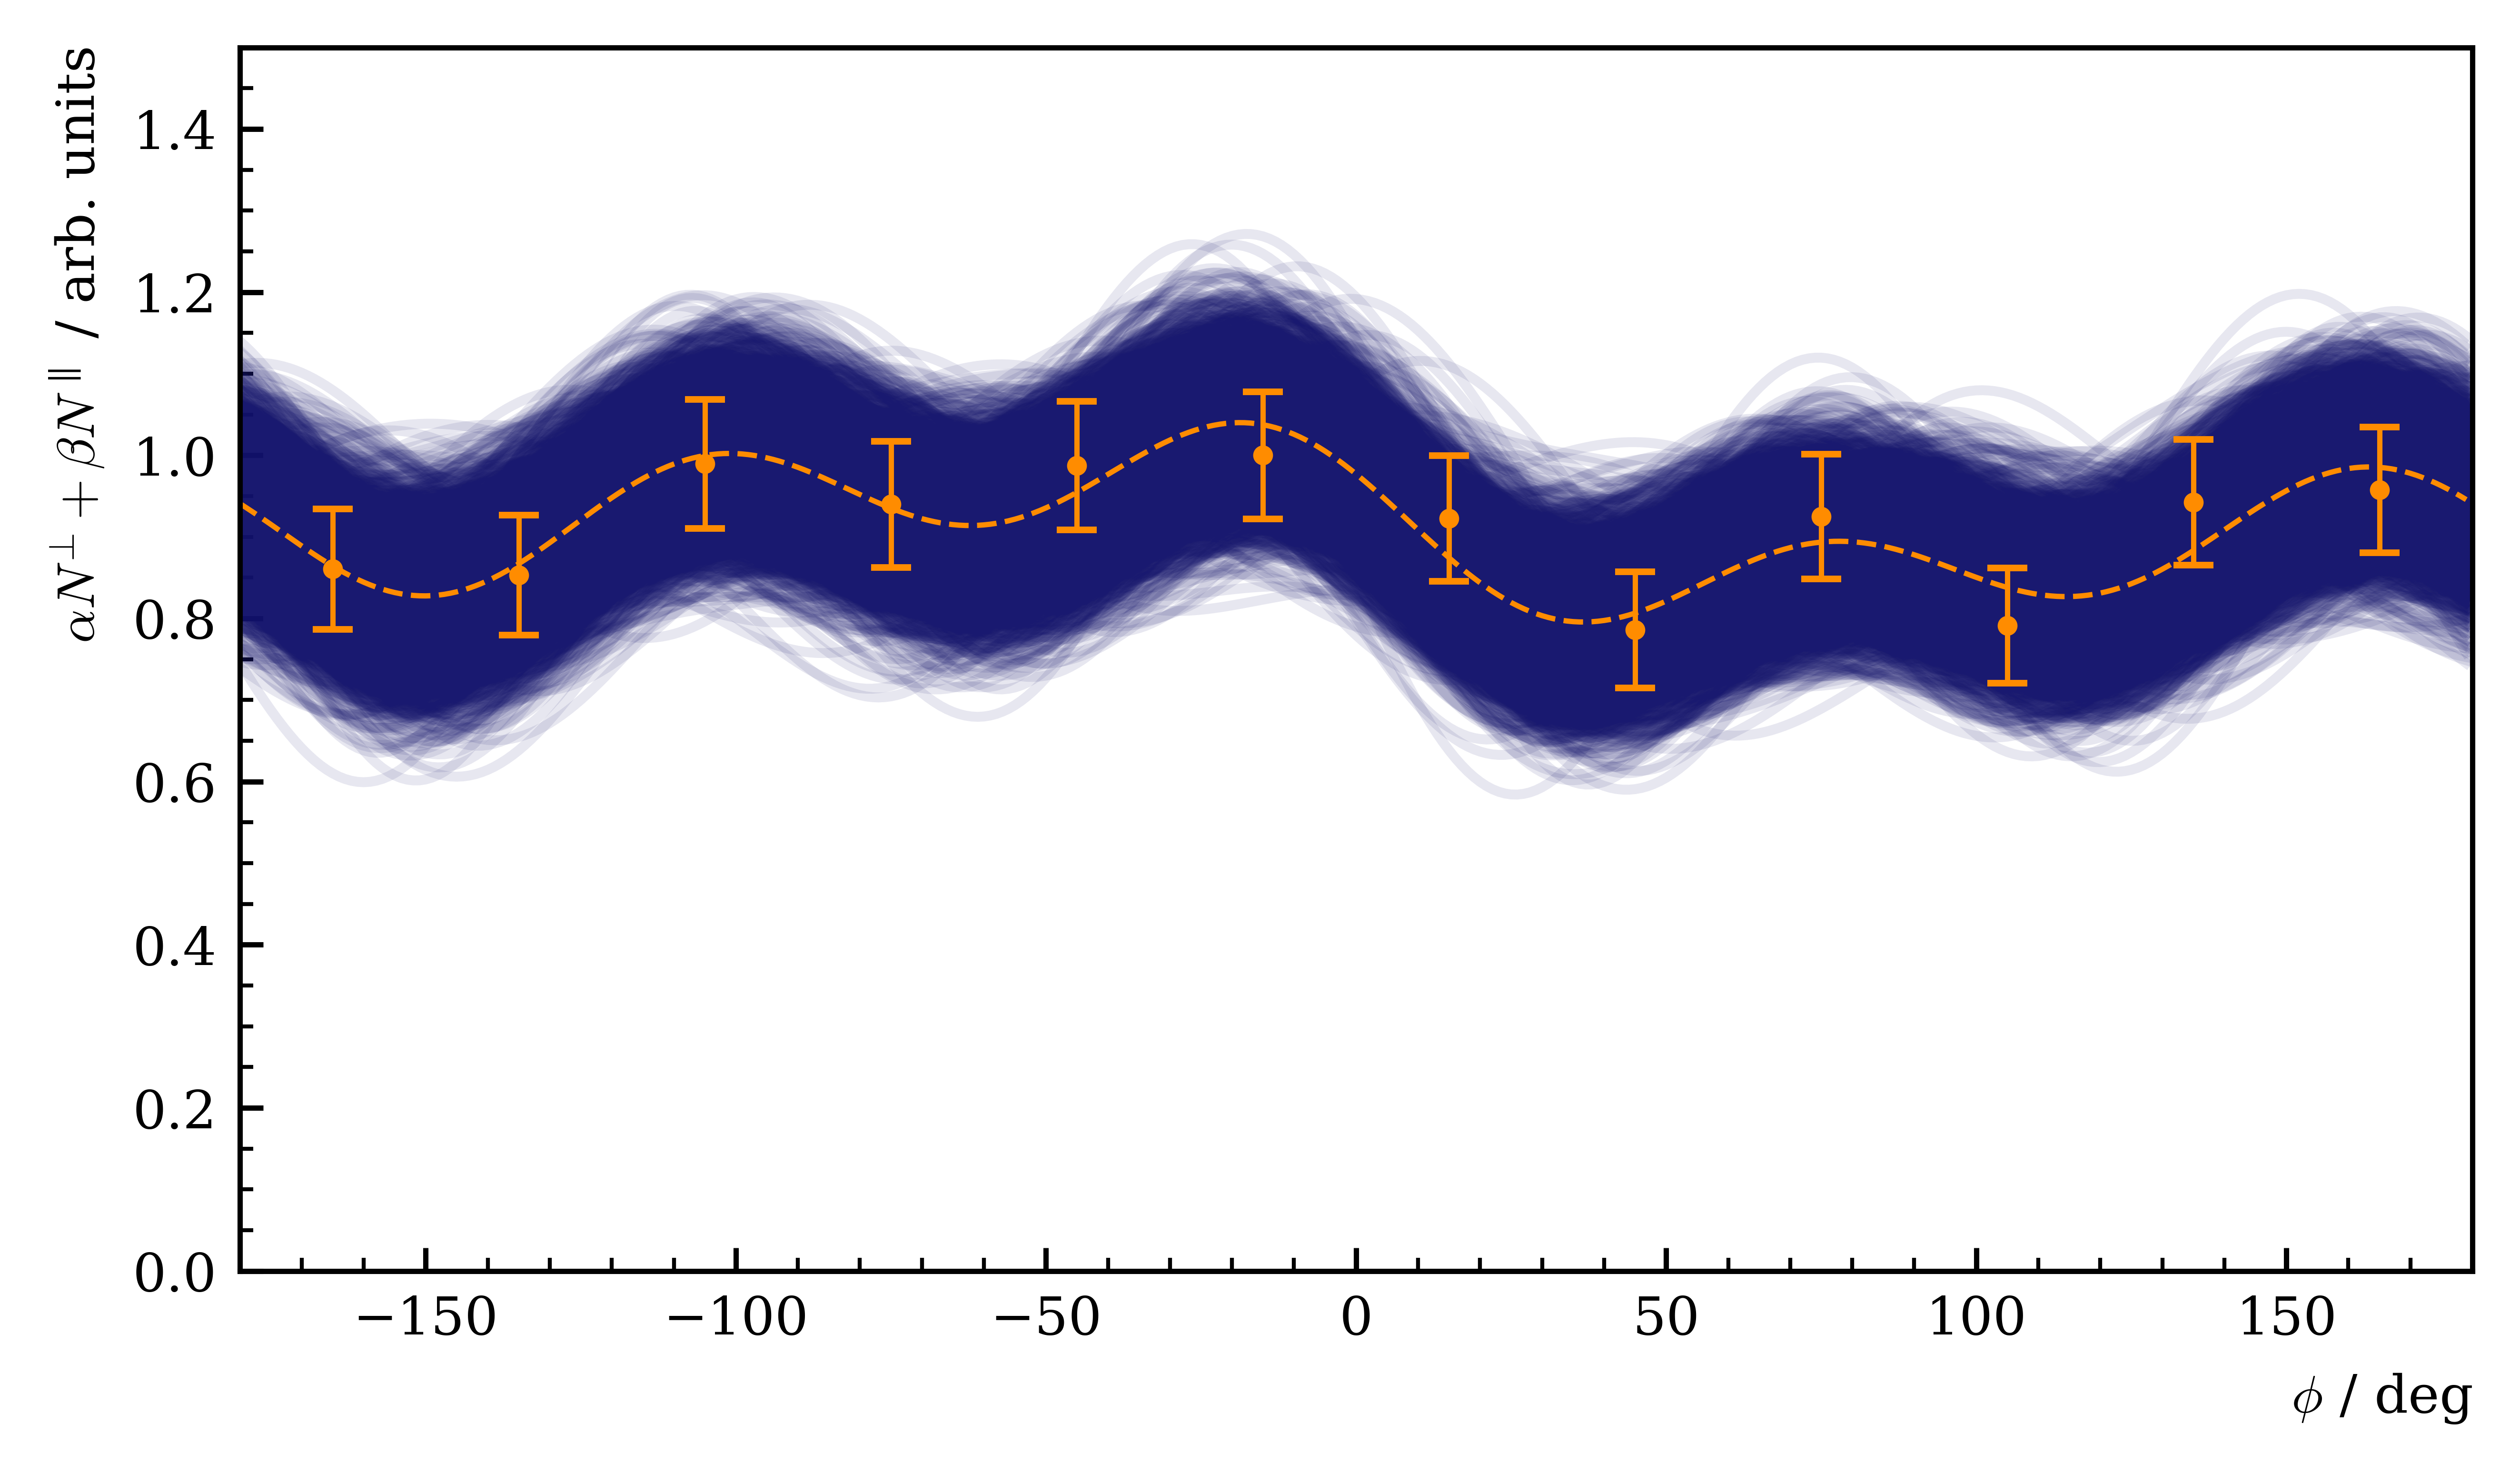
\includegraphics[width=\linewidth]{../bayes/event_based_fit/plots/toyMC_eff_PPC.png}
	\caption{Posterior predictive check using the draws of the detector coefficients $a$ and $b$. Points with error bars are the polarization weighted sum of event yields. The dashed line is the mean of the predictive values while the solid opaque lines are representative of one simulation draw $a^{(s)},b^{(s)}$.}
	\label{fig:toyMC_eff_func}
\end{figure}
As opposed to the binned fit it is not only performed at each data point but for significantly more points. This mimics a continuous function as is appropriate for an unbinned fit. However, for better visibility the posterior predictive distributions are not built at every point but the efficiency function is plotted for each set of draws $a^{(s)},b^{(s)}, s=1\dots4000$. No $p$ values are estimated since they would not be representative of the whole fit. The mean of the posterior predictive distributions is given by the dashed line and agrees within statistical error bars with the simulated data.
\newpage
\subsection{Application of methods to data}
Since both methods were tested successfully using toy Monte Carlo data, both are subsequently applied to real data to extract the beam asymmetry. Since the number of fits is small compared to the amount of fits performed during testing, the amount of posterior draws was increased to $5000$ per chain. All other hyperparameters were left the same
\begin{align}
	n_\text{samples}=5000 && n_\text{chain}=4 && n_\text{warm up}=1000.
\end{align}
\subsubsection{Event yield asymmetries}
In all bins of beam energy and meson polar angle the binned fit was performed. Similar to the Monte Carlo samples, 12 bins in phi are built to comply with the binning in reference \cite{farahphd}, and guarantee comparability.

Figure \ref{fig:asym} shows the resulting asymmetry $A(\phi)$ for all angular bins for the energy bin $\SI{1250}{\mega\eV}\leq E_\gamma<\SI{1310}{\mega\eV}$ as orange data points with statistical error bars.  Additionally, a $\chi^2$ fit (orange line) to the asymmetry together with posterior predictive checks as obtained from a fully \textsc{Bayesian} fit according to the introduced model (blue distributions) is shown. The goodness of fit is checked via the introduced $p$-values $p=T(A_\text{rep}>A)$, and are shown as black points with propagated error bars on the bottom. The optimal value of $p=0.5$ is marked by the dashed line and realizes the mean of the distribution of all $p$-values, so that one can assume good description of the data by the fits, see Figure \ref{fig:pvals}. This replaces the investigation of the $\chi^2/\text{NDF}$ distribution in the case of a frequentist fit.   

\begin{sidewaysfigure}[htbp]
		\centering
		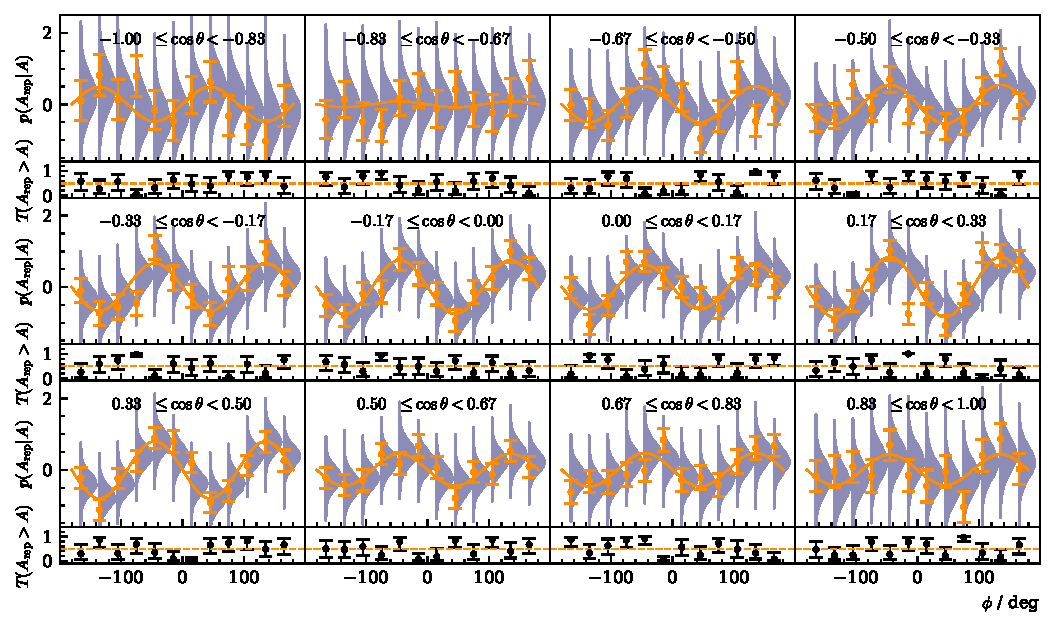
\includegraphics[width=\linewidth]{../bayes/realdeal/plots/ppd_checks.pdf}
		\caption{Posterior predictive checks $p\left(A_\text{rep}\big|A\right)$ from a \textsc{Bayesian} fit to the event yield asymmetries for the reaction $\gamma p\to p\eta\to p\gamma\gamma$ for all angular bins of the energy bin $\SI{1250}{\mega\eV}\leq E_\gamma<\SI{1310}{\mega\eV}$. The data points in the upper plot are the asymmetry $A\left(\phi\right)$, which was additionally fitted using a $\chi^2$ fit (solid line). The goodness of fit is shown using $p$-values, which give the fraction $T\left(A_\text{rep}>A\right)$ of replicated samples greater than the original measured value, with propagated statistical error bars on the bottom of each plot. The expected mean value of $T\left(A_\text{rep}>A\right)=0.5$ is indicated by the dashed line. }
		\label{fig:asym}
\end{sidewaysfigure}


\begin{figure}[htbp]
	\centering
	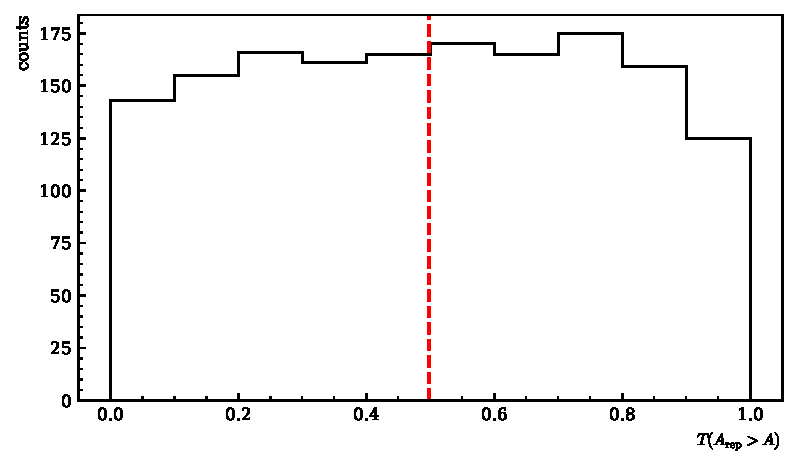
\includegraphics[width=\linewidth]{../bayes/realdeal/plots/pval_hist.pdf}
	\caption{$p$ values generated using all fits from all bins in the reaction $\gamma p\to p\eta\to p\gamma\gamma$. They are centered around their mean at $0.5$, which is indicated by the dashed line, and show no bias towards higher or lower values, thus confirming an adequate fit.}
	\label{fig:pvals}
\end{figure}
The MCMC diagnostics reveal that all \textsc{Markov} chains have converged and explored the available parameter space completely which is characterized by $\widehat{R}=1.00$ for all fits. The increment of posterior draws removed any fluctuations in the $\widehat{R}$ value that was present before. The relative MCSE is below the (self-)defined threshold of $\frac{\sigma_\text{MCSE}}{\text{median}\left[p\left(\Sigma|y\right)\right]}<5\%$ for $95\%$ of all fits. The remaining $5\%$ are fits that estimated the beam asymmetry close to $0$ such that further incrementing the number of posterior draws will not amend this. Both, relative MCSE and $\widehat{R}$ associated with the fit parameter $\Sigma$ of the binned fit, are shown in Figure \ref{fig:diagnostics}. Thus, one can conclude the successful tuning of hyperparemeters concerning the \textsc{Bayesian} fit. 
\begin{figure}[htbp]
	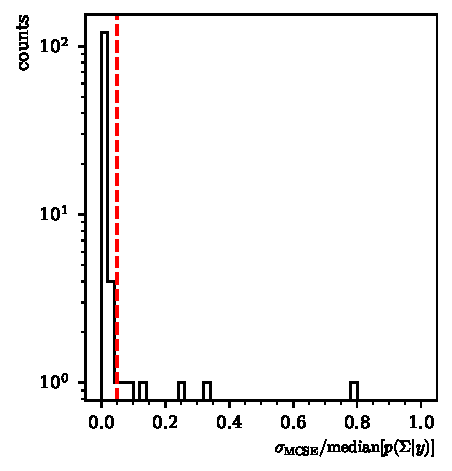
\includegraphics[width=.49\linewidth]{../bayes/realdeal/plots/mcse_hist.pdf}
	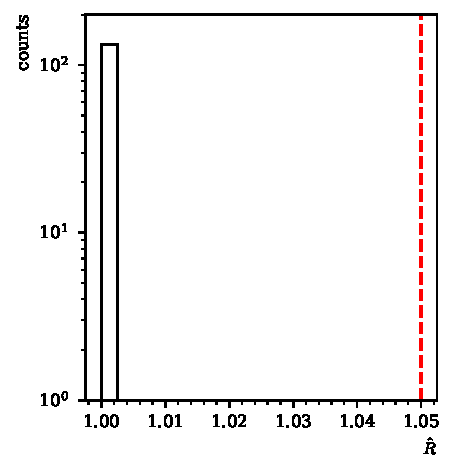
\includegraphics[width=.49\linewidth]{../bayes/realdeal/plots/rhat_hist.pdf}
	\caption{ Left: relative error $\frac{\sigma_\text{MCSE}}{\text{median}\left[p\left(\Sigma|y\right)\right]}$ Right: $\widehat{R}$ associated with the fit parameter $\Sigma$. Both are shown for all $11\cdot12$ binned \textsc{Bayesian} fits to the asymmetry $A\left(\phi\right)$ in $\eta$ photoproduction. The critical values that should not be exceeded are marked by dashed lines.}
	\label{fig:diagnostics}
\end{figure}
\subsubsection{Event based fit}
The discussed \textsc{Bayesian} event based fit is also performed for all kinematic bins. The MCMC diagnostics reveal good choice of hyperparameters, as Figure \ref{fig:diagnostics1} shows. As already observed during the toy Monte Carlo experiments, the unbinned fit produces more precise results; $98\%$ of all fits exhibit an MCSE below threshold, those bins with error above threshold are again explained by values of the beam asymmetry $\Sigma\approx0.$ Good within and between chain convergence is reached, as $\widehat{R}=1.00$ for all fits shows.

The only illustrative measure regarding the performance of the unbinned fit is the posterior predictive distribution of the detector coefficients $a,b$. Figure \ref{fig:eff_func} shows the weighted sum of event yields with the same binning as used in the binned fit together with a posterior predictive check using the draws of all parameters distributions $a,b$ for the kinematic bin $\SI{1250}{\mega\eV}\leq E_\gamma<\SI{1310}{\mega\eV}, 0\leq\cos\theta<0.17$. 
As opposed to the binned fit it is not only performed at each data point but for significantly more points. This mimics a continuous function as is appropriate for an unbinned fit. However, for better visibility the posterior predictive distributions are not built at every point but the efficiency function is plotted for each set of draws $a^{(s)},b^{(s)}, s=1\dots20000$. No $p$ values are estimated since they would not be representative of the whole fit. Note that the detector efficiency $\epsilon\left(\phi\right)$ is almost flat as opposed to the simulated efficiency in subsection \ref{subsec:toyMC}. This is an overall observation and not specific to the shown kinematic bin and further confirmed by the fact that the sums of all fit coefficients $a,b$ are distributed around zero. Regardless of the significance of detection inefficiencies the unbinned fit is nevertheless able to obtain good agreement between fit and data; the mean of all posterior predictive distributions (dashed line) agrees within statistical error bars with the data points.
 \begin{figure}[htbp]
	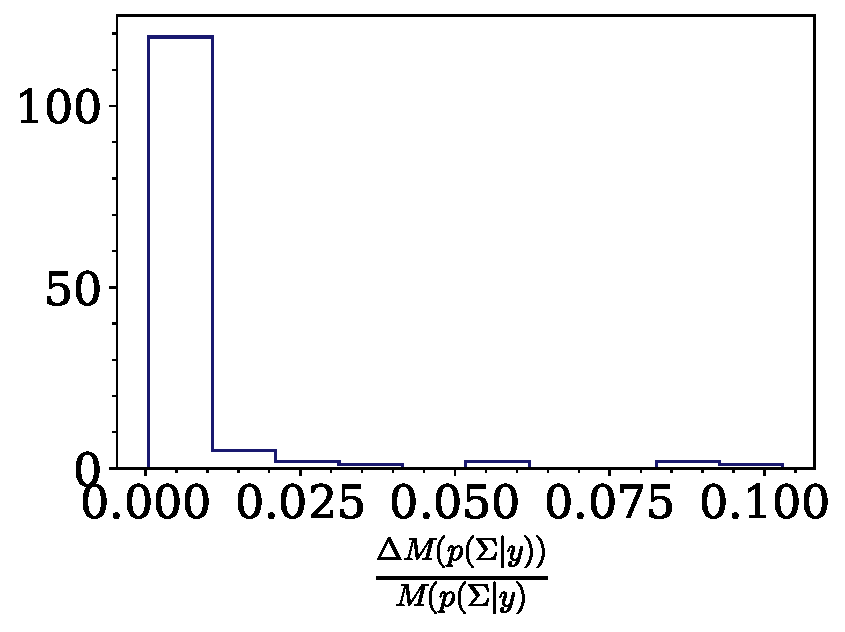
\includegraphics[width=.49\linewidth]{../bayes/event_based_fit/plots/mcse_hist.pdf}
	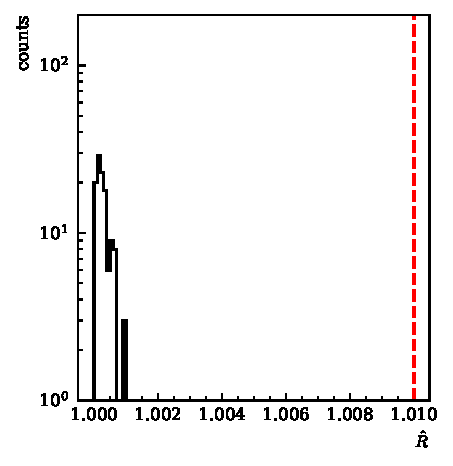
\includegraphics[width=.49\linewidth]{../bayes/event_based_fit/plots/rhat_hist.pdf}
	\caption{ Left: relative error $\frac{\sigma_\text{MCSE}}{\text{median}\left[p\left(\Sigma|y\right)\right]}$ Right: $\widehat{R}$ associated with the fit parameter $\Sigma$. Both are shown for all $11\cdot12$ unbinned fits in $\eta$ photoproduction. The critical values that should not be exceeded are marked by dashed lines.}
	\label{fig:diagnostics1}
\end{figure}
\begin{figure}[htbp]
	\centering
	
\includegraphics[width=\linewidth]{../bayes/event_based_fit/plots/eff_PPC.png}
	\caption{Posterior predictive check using the draws of the detector coefficients $a$ and $b$ for the kinematic bin $\SI{1250}{\mega\eV}\leq E_\gamma<\SI{1310}{\mega\eV}, 0\leq\cos\theta<0.17$. Points with error bars are the polarization weighted sum of event yields. The dashed line is the mean of the predictive values while the solid opaque lines are representative of one simulation draw $a^{(s)},b^{(s)}$.}
	\label{fig:eff_func}
\end{figure}
\subsection{Discussion}
\label{sec:sigma_eta}
The final results for the beam asymmetry obtained with both methods are shown in Figure \ref{fig:eta_res} for all bins in beam energy and meson polar angle. Along with the marginal posterior distributions obtained from both introduced methods point estimates from a $\chi^2$ fit and an unbinned fit \cite{farahphd} are shown. An important intermediate result is that all results agree with each other within statistical error bars or within the width of the marginal posterior distributions. Any effects that lead to slightly distinguishable point estimates from a binned or unbinned fit are propagated directly throughout the \textsc{Bayesian} fit; then each distribution is centered around the point estimate of the respective fitting method. The results from the binned and unbinned fit with error bars on average cover $68\%$ of the respective marginal posterior distributions, corresponding to a $1\sigma$ interval. Thus, in general, the application of \textsc{Bayesian} methods has proven to give the same results and no systematic error is introduced by the \textsc{Bayesian} approach. 
	\begin{sidewaysfigure}[htbp]
	\centering
	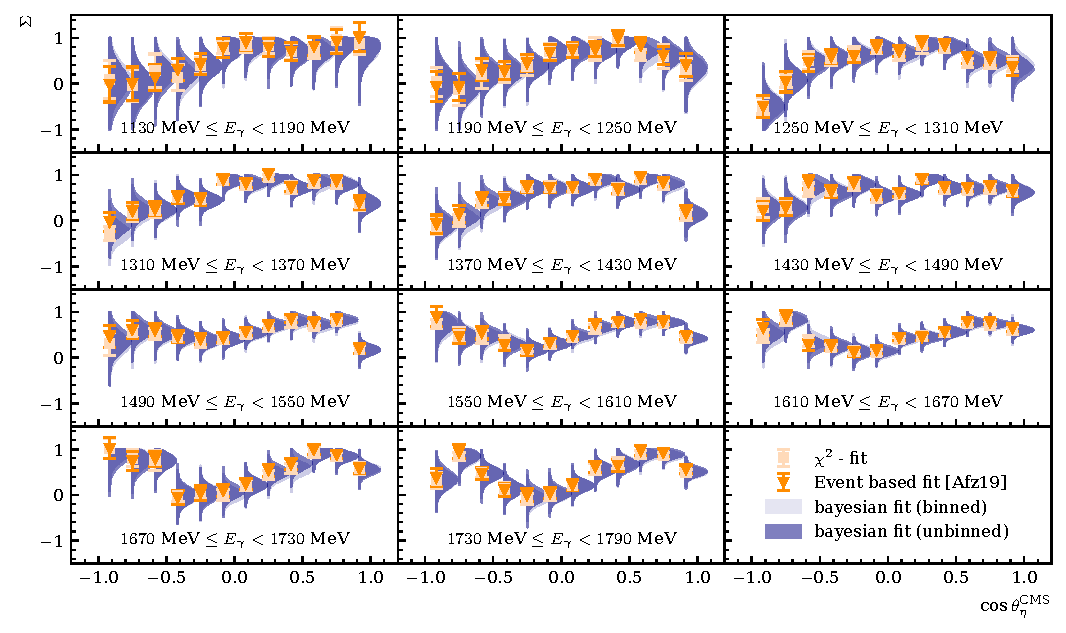
\includegraphics[width=\linewidth]{../bayes/event_based_fit/plots/sigma_eta.pdf}
	\caption{Final results for the beam asymmetry $\Sigma$ in $\eta$ photoproduction off the proton for all kinematic bins obtained with \textsc{Bayesian} methods. They are compared with the results of a least squares fit and an unbinned fit as given in reference \cite{farahphd}. All results agree within statistical error bars or within the widths of marginal posterior distributions.}
	\label{fig:eta_res}
\end{sidewaysfigure}
The effort of implementing the binned or unbinned fit in a \textsc{Bayesian} approach is comparable to using standard libraries provided by e.g. \emph{python} \cite{python} or \emph{ROOT} \cite{root}. Due to the probabilistic structure of the Stan language \cite{stan} implementation of likelihood and prior models is straightforward and the sampling algorithms can be accessed or modified to ones needs intuitively. However, the \textsc{Bayesian} fit requires more careful preparation and also diagnostics. On one hand, the choice of priors has to be made. On the other hand, the fitting procedure is inherently different; not only the goodness of fit compared with data has to be checked but also the convergence of the \textsc{Markov} chains themselves. 

The computational cost also increases greatly in comparison to the traditional frequentist approaches. Especially the unbinned \textsc{Bayesian} fit requires a lot of computation time,  where the number of data points is of order $\mathcal{O}(10^4)$ as opposed to 12 data points for the binned fit. This can be understood considering the underlying algorithms; the least squares fit and also the unbinned maximum likelihood fit both aim to minimize a given test statistic which is achievable by differentiation. Determining marginal posterior distributions from \textsc{Bayesian} inference on the other hand requires (numeric) integration, making it the more complex task which is observable in the consumed computation time. While an unbinned maximum likelihood fit using e.g. \texttt{TTree::UnbinnedFit} \cite{runbinnedFit} takes seconds, the \textsc{Bayesian} unbinned fit took up to 20 minutes. 

Yet, the additional effort is rewarded by the fact that the \textsc{Bayesian} fit will yield \emph{distributions} for all parameters as opposed to point estimates with error bars. This is especially useful for polarization observables which may be used as input for PWA calculations. Here error estimates can be derived from the distributions e.g. as (multiple) standard deviations, the full width at half maximum or similar. If furthermore a \textsc{Bayesian} approach is  pursued, also the whole distributions may be used. Because the final results are distributions also the structure of these may be analyzed uncovering possible multimodalities as well as distributions diferring from i.e. a symmetric \textsc{Gaussian}. Another advantage of the \textsc{Bayesian} fit is the ability to truncate the posterior samples to the relevant or allowed parameter space. In the very first energy bin in Figure \ref{fig:eta_res} this is visible clearly where several point estimates exceed the physical limit of $\Sigma=1$ as opposed to the obtained marginal posteriors. Lastly, the \textsc{Bayesian} fit allows much more flexible changes to the fitted model, as will be discussed in the next section \ref{sec:sigma_etap}.


      
\section{Determination of $\Sigma_{\eta'}$}
\label{sec:sigma_etap}
After successfully testing the application of \textsc{Bayesian} methods this section will demonstrate the extraction of new results for the beam asymmetry in $\eta'$ photoproduction off the proton obtained at the CBELSA/TAPS experiment. Only the event based fitting method is applied and the binned fitting of event yield asymmetries is discarded because on the one hand the available statistics will on average give only few counts per bin $\left(E_\gamma,\cos\theta,\phi\right)$ of order $\mathcal{O}\left(10^1\right)$, depending on the specific number of $\phi$-bins. This will result in very large statistical errors per bin that may also not necessarily approximated as \textsc{Gaussian} anymore. On the other hand this could be compensated by choosing fewer bins in $\phi$ which would however amplify the systematic underestimation of the beam asymmetry which is discussed in appendix \ref{app:binnedfits}.

The event based fits are performed as unbinned maximum likelihood fit and as an unbinned \textsc{Bayesian} fit. New toy Monte Carlo experiments are thrown adapting to the significantly decreased statistics. Also, tests regarding the background contamination of Monte Carlo samples are made, see Chapter \ref{chap:events}.   
\subsection{Application of event based fit to toy Monte Carlo data}
After selecting all suitable event candidates for $\gamma p \to p \eta'\to p\gamma\gamma$ reactions there still remain significant background contributions which make up roughly $20\%$ of all events averaged over all kinematic bins. Investigation of Monte Carlo simulations of different mesonic final states revealed they are mainly realized by the false reconstruction of $2\pi^0$ photoproduction events (see chapter \ref{chap:events}). It was thus investigated how the presence of two beam asymmetries $\Sigma_1$ and $\Sigma_2$ affects the fit. The combined differential cross section is then given by \begin{align}
	\frac{\text{d}\sigma}{\text{d}\Omega}_\text{pol}\left(\phi\right)&=\frac{\text{d}\sigma}{\text{d}\Omega}_\text{pol}^{(1)}\left(\phi\right)+\frac{\text{d}\sigma}{\text{d}\Omega}_\text{pol}^{(2)}\left(\phi\right)\\&=\frac{\text{d}\sigma}{\text{d}\Omega}_0^{(1)}\cdot\left(1-p_\gamma\Sigma_1\cos\left(2\phi\right)\right)+\frac{\text{d}\sigma}{\text{d}\Omega}_0^{(2)}\cdot\left(1-p_\gamma\Sigma_2\cos\left(2\phi\right)\right).
	\label{eq:asym1}
\end{align}
If now the fraction $\delta$ of events in the final state with beam asymmetry $\Sigma_2$ is known one can express the unpolarized cross sections via a common combined unpolarized cross section as
\begin{align}
	\frac{\text{d}\sigma}{\text{d}\Omega}_0^{(1)}=\left(1-\delta\right)\cdot\frac{\text{d}\sigma}{\text{d}\Omega}_0&&\frac{\text{d}\sigma}{\text{d}\Omega}_0^{(2)}=\delta\cdot\frac{\text{d}\sigma}{\text{d}\Omega}_0.
	\label{eq:delta}
\end{align}
Plugging Equation \eqref{eq:delta} into Equation \eqref{eq:asym1} then yields
\begin{equation}
	\frac{\text{d}\sigma}{\text{d}\Omega}_\text{pol}\left(\phi\right)=\frac{\text{d}\sigma}{\text{d}\Omega}_0\cdot\left(1-p_\gamma\left[\left(1-\delta\right)\cdot\Sigma_1+\delta\cdot\Sigma_2\right]\cos\left(2\phi\right)\right).
\end{equation}
In the presence of background $\Sigma^\text{bkg}$\footnote{For clarity, the beam asymmetry associated with random time background will in this section be denoted as $\Sigma^\text{bkg}_t$ and the beam asymmetry associated with background reactions as $\Sigma^\text{bkg}$.} all measured values for the beam asymmetry $\Sigma^\text{meas}$ are systematically shifted from their true value $\Sigma^\text{true}$, depending on the amount of background, if the methods described in section \ref{sec:meth} are used without modification, i.e.
\begin{equation}
	\Sigma^\text{meas}=\left(1-\delta\right)\cdot\Sigma^{\text{true}}+\delta\cdot\Sigma^{\text{bkg}}.
	\label{eq:sigmeas}
\end{equation}
This is an important intermediate result: If the background asymmetry $\Sigma^\text{bkg}$ and the corresponding fraction of events $\delta$ that exhibit this asymmetry are known, the true values $\Sigma^\text{true}$ can be obtained. If $\Sigma^\text{bkg}$ is not known this is a source of systematic error.

Table \ref{tab:mcsum1} shows all characteristics of the investigated toy Monte Carlo experiments, the values for polarization and statistics per bin were chosen to match the respective average values in the selected data for the $\gamma p \to p\eta'\to p\gamma\gamma$ final state. Furthermore $\delta=20\%$ of all events were simulated as background with beam asymmetry $\Sigma_2$ while the remainder of events is simulated with beam asymmetry $\Sigma_1$. The amount of random time background in the prompt peak is set to $(1-f)=0.05$ while the sideband events are weighted by $w=\frac{13}{200}$ (see section \ref{sec:time}). The same efficiency function and hyperparameters are employed as previously with the exception of the number of posterior draws which is raised to $n_\text{samples}=5000$ from the beginning. Because of the smaller amount of data this does not increase the computational cost immensely.
\begin{table}[htbp]
	
	\renewcommand{\arraystretch}{1.5}
	\centering
	\begin{tabularx}{\linewidth}{l|XXX}
		\toprule
		\textbf{chosen parameters} & \multicolumn{3}{l}{$p_\gamma^\parallel=0.3,p_\gamma^\bot=0.3,\Sigma_1=0.5$, $\Sigma_2=-0.3$,$\Sigma$ $\Sigma^\text{bkg}_t=-0.5$, $f=0.95$, $\delta=0.2$}\\ &\multicolumn{3}{l}{$w=\frac{13}{200}$}\\
		\hline
		\textbf{simulation draws} &\multicolumn{3}{c}{$ N^\parallel_{\text{total}}\sim\mathcal{P}(200)$, $ N^\bot_{\text{total}}\sim\mathcal{P}(200)$}\\
		\cline{2-4}
		&signal in prompt&background in prompt& sideband \\
		&$N^{\parallel/\bot}_\text{total}\cdot f$&$N^{\parallel/\bot}_\text{total}\cdot\left(1-f\right)$&$N^{\parallel/\bot}_\text{total}\cdot\left(1-f\right)\cdot1/w$\\
		\hline
		\textbf{efficiency function}&\multicolumn{3}{l}{$\epsilon\left(\phi\right)=1/10.5\cdot\left(9.3+0.28\cdot\cos\phi+0.24\cdot\sin3\phi\right)$}\\
		\hline
		\textbf{hyperparameters}&\multicolumn{3}{l}{$n_\text{samples}=5000,n_\text{chain}=4,n_\text{warm up}=1000$}\\
		\bottomrule
	\end{tabularx}
	\caption{Summary of the complete setting of all toy Monte Carlo experiments for the event based fit. Table layout adapted from \cite{farahphd}.}
	\label{tab:mcsum1}
\end{table}
\subsubsection{Unbinned maximum likelihood fit}
To test the unbinned maximum likelihood fit and its response to the presence of background, 10000 toy Monte Carlo bins are created according to table \ref{tab:mcsum1}. The expected beam asymmetry is \begin{equation}
	\Sigma^\text{meas}=0.8\cdot0.5-0.2\cdot0.3=0.34.
\end{equation} 
Building the normalized residuals with respect to $\Sigma^\text{meas}$ and the random time background asymmetry $\Sigma^\text{bkg}_t$ yields standard normal distributions, see Figures \ref{fig:ml_sigma} and \ref{fig:ml_sigmat}, thus fulfilling the expectations entirely. This allows Equation \eqref{eq:sigmeas} to be applied on results obtained with this method provided the background beam asymmetry is known. Any errors on $\Sigma^\text{bkg}$ may be propagated in a \textsc{Gaussian} manner. The beam asymmetry is estimated without bias and the errors are correctly estimated as confirmed by $\mu=0$ and $\sigma=1$ for the normalized residuals within few widths of the statistical errors. Note that the unnormalized distributions are significantly broader than the ones examined in the previous section which is due to the decreased statistics in each bin which already indicates larger statistical errors. The decreased statistics also cause greater variation in the fitted efficiency function that is seen in Figure \ref{fig:toyMCeff}, which still describes the data very well.
\begin{figure}[htbp]
	\centering
	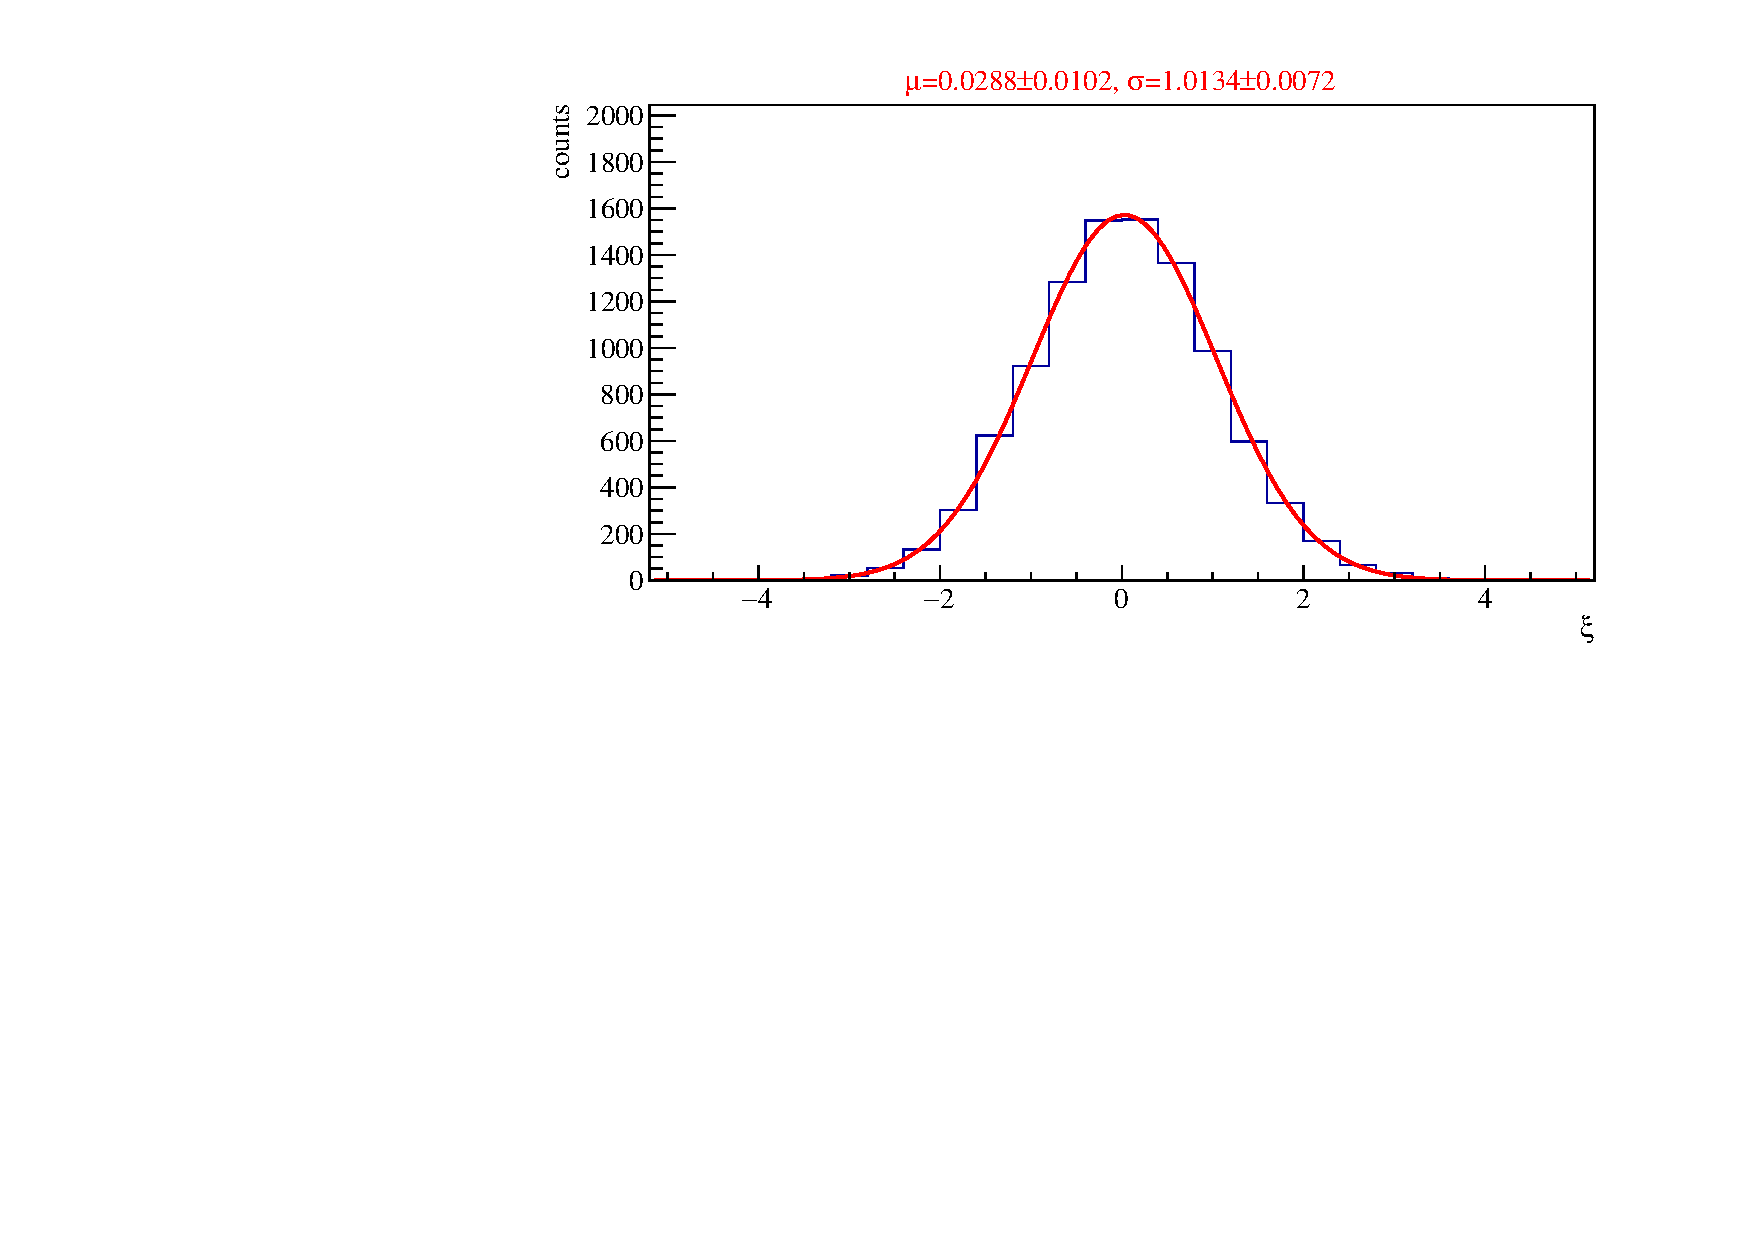
\includegraphics[width=.49\linewidth]{../RooFit/plots/residuals.pdf}
	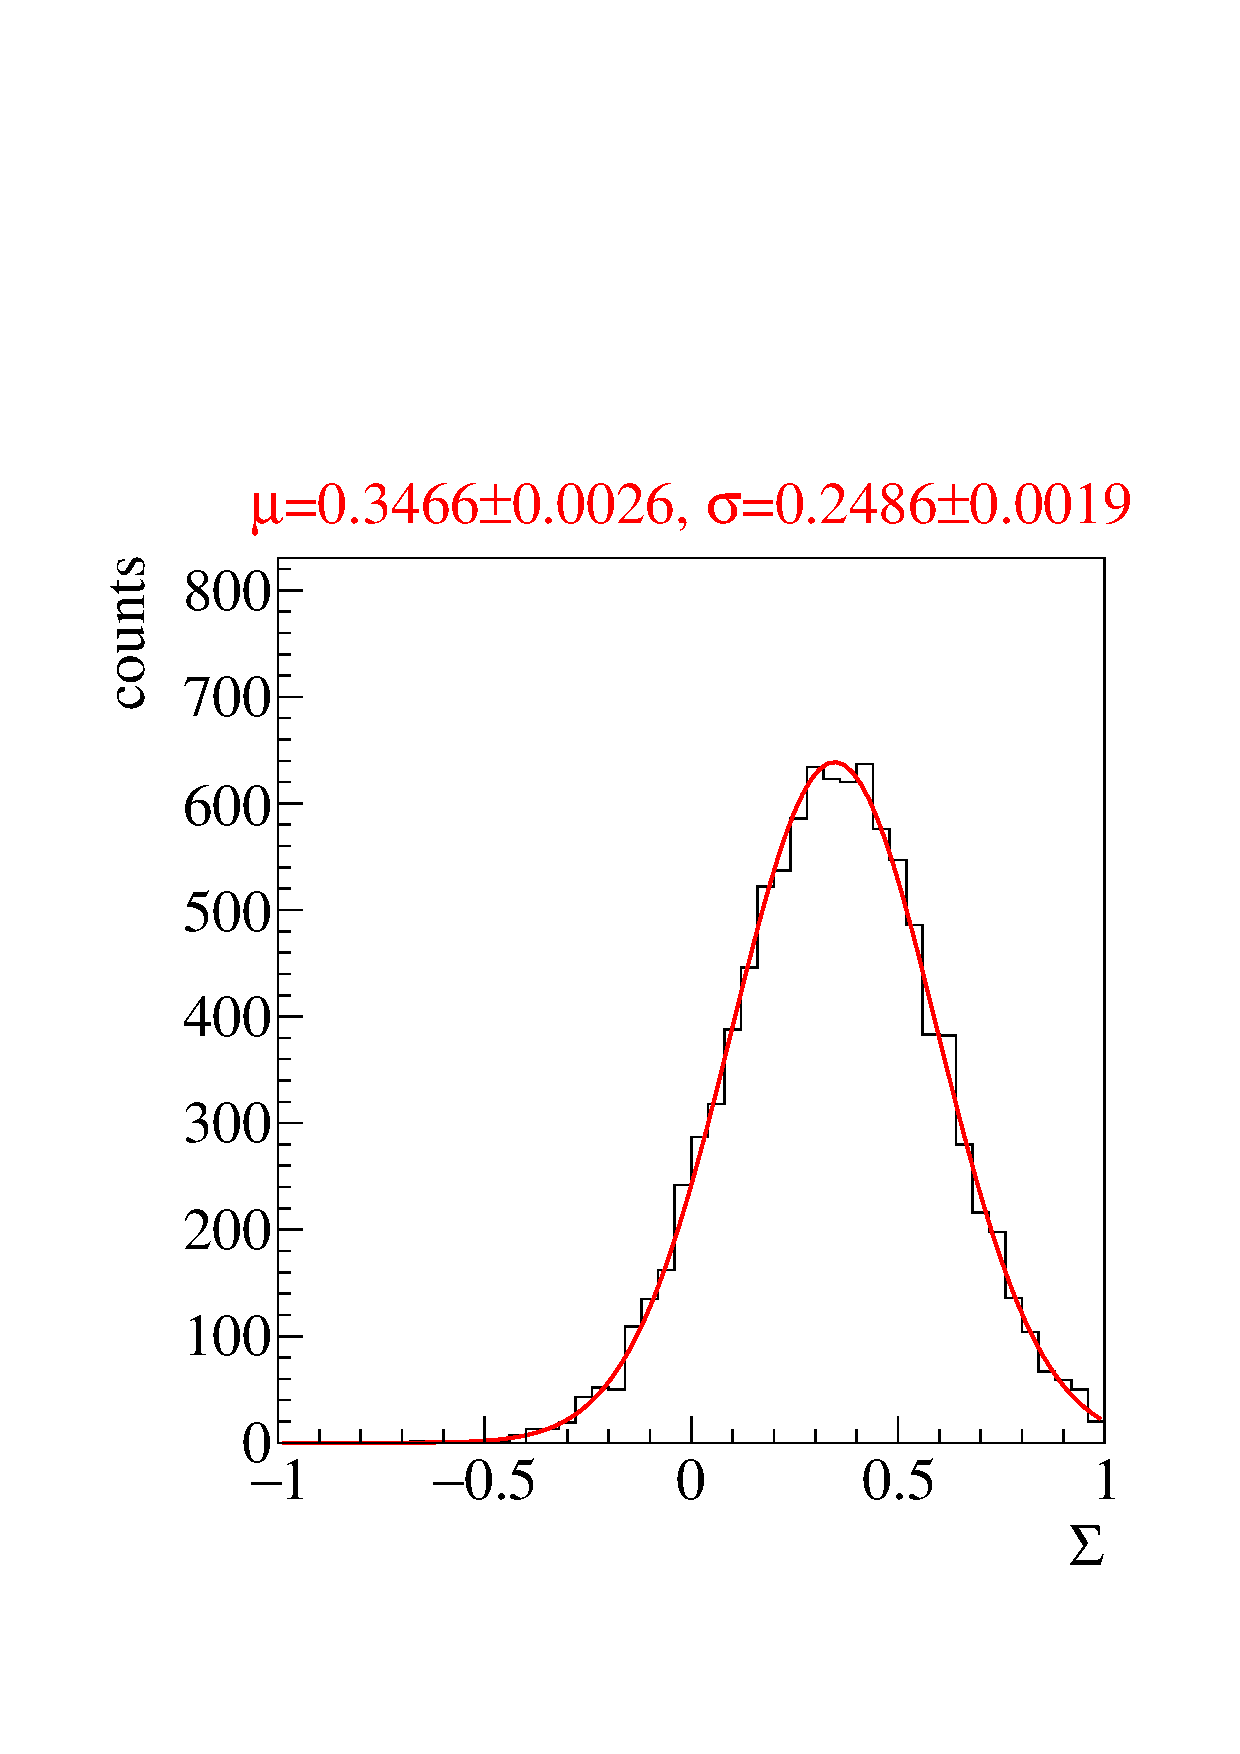
\includegraphics[width=.49\linewidth]{../RooFit/plots/sigma.pdf}
	\caption{Normalized residuals (left) and unaltered distribution (right) of all 10000 fits for the beam asymmetry $\Sigma=(1-\delta)\cdot\Sigma_1+\delta\cdot\Sigma_2$. \textsc{Gaussian} fits are performed with results given on top of each plot.}
	\label{fig:ml_sigma}
\end{figure}
\begin{figure}[htbp]
	\centering
	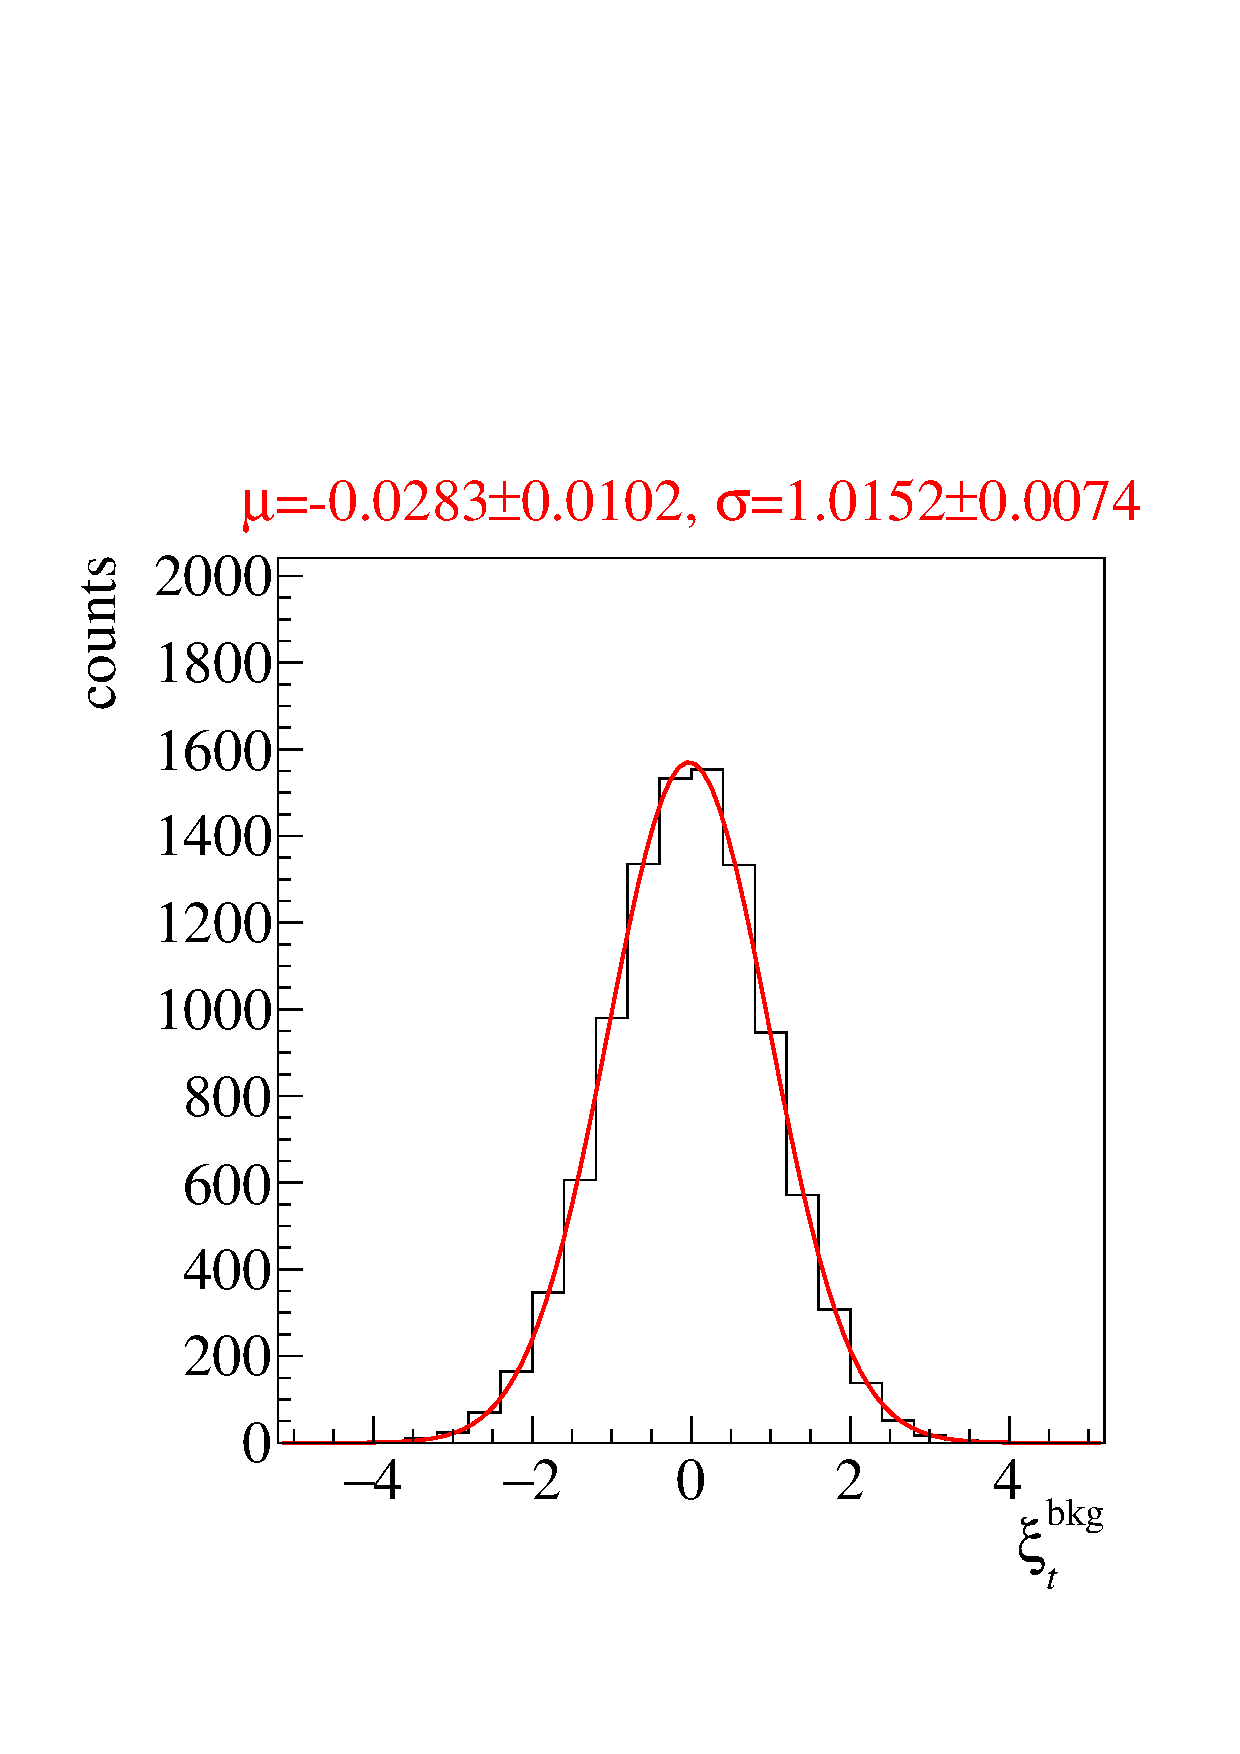
\includegraphics[width=.49\linewidth]{../RooFit/plots/residuals_bkg.pdf}
	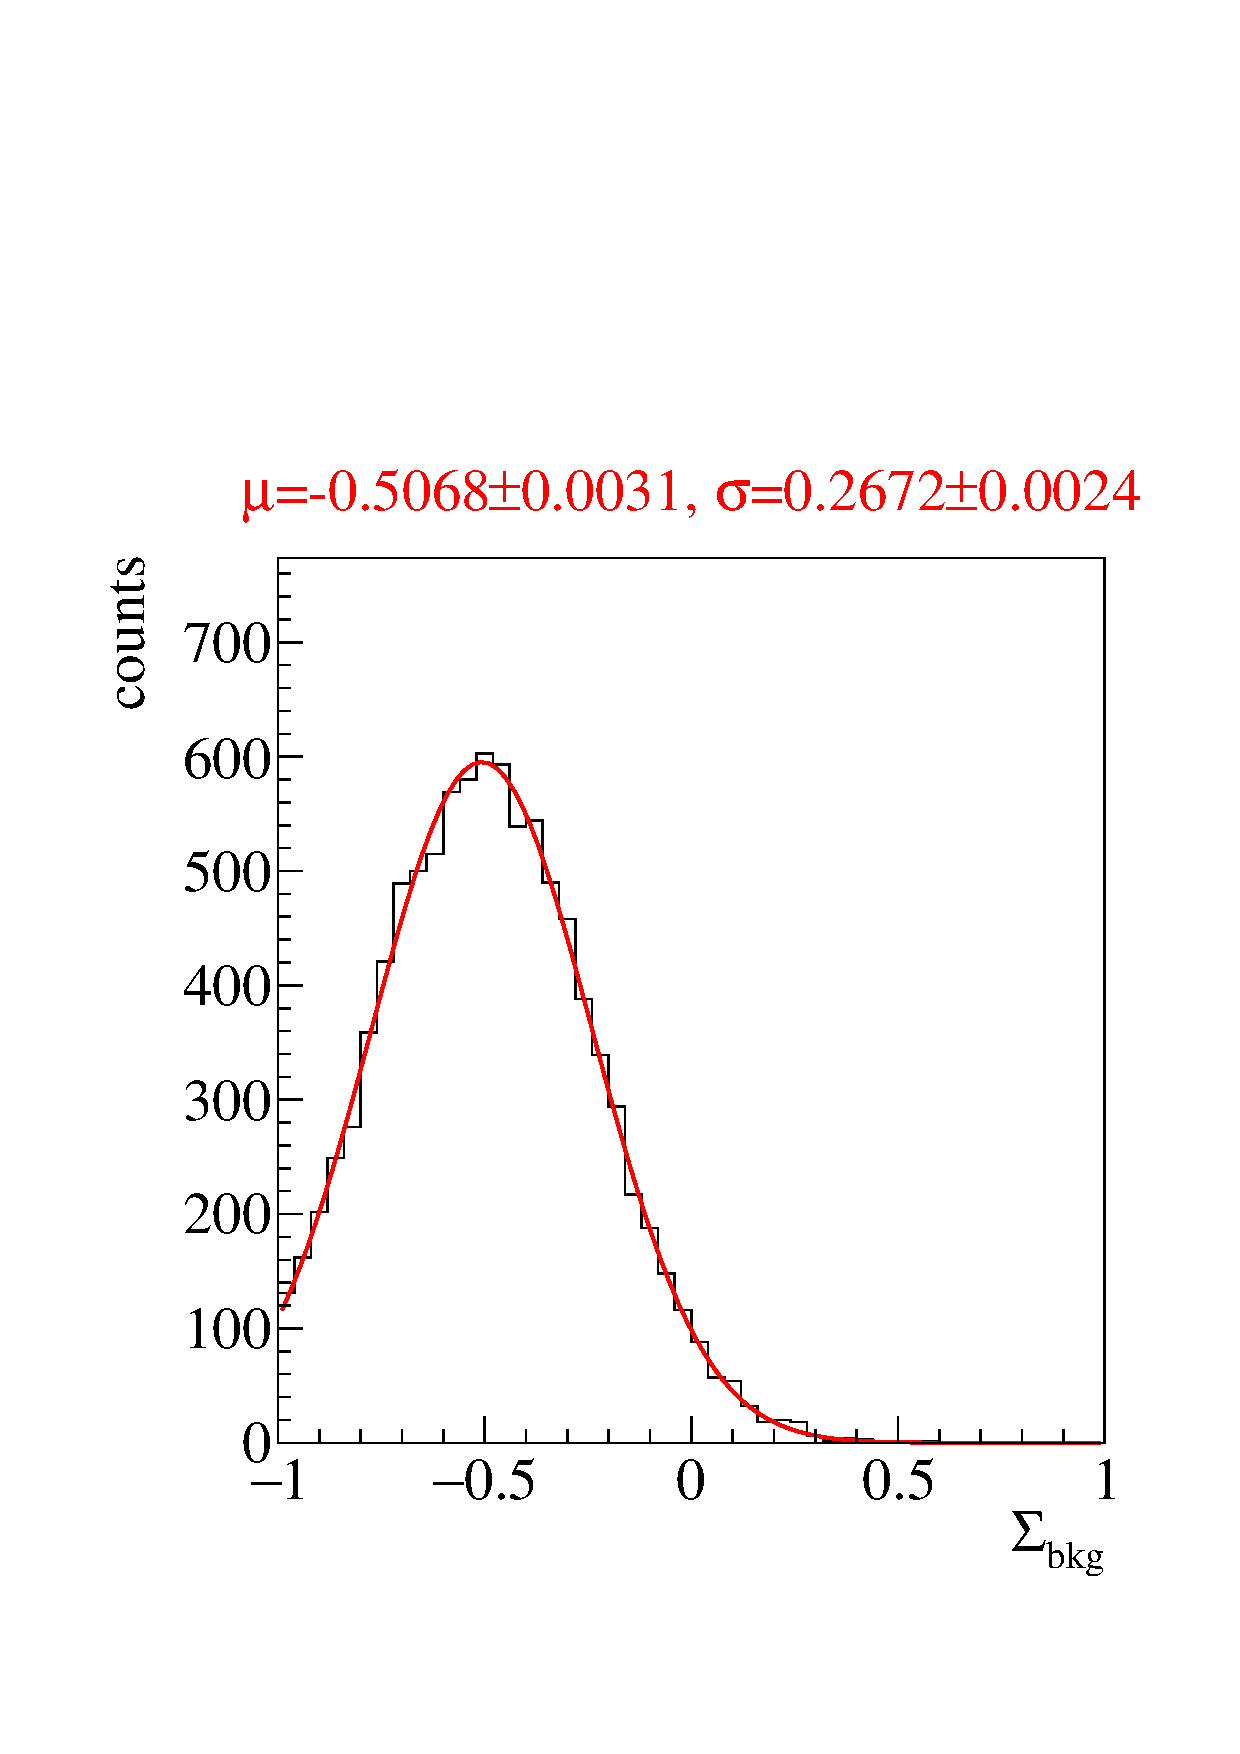
\includegraphics[width=.49\linewidth]{../RooFit/plots/sigma_bkg.pdf}
	\caption{Normalized residuals (left) and unaltered distribution (right) of all 10000 fits for the background beam asymmetry $\Sigma^\text{bkg}_t$. \textsc{Gaussian} fits are performed with results given on top of each plot.}
	\label{fig:ml_sigmat}
\end{figure}
\begin{figure}[htbp]
	\centering
	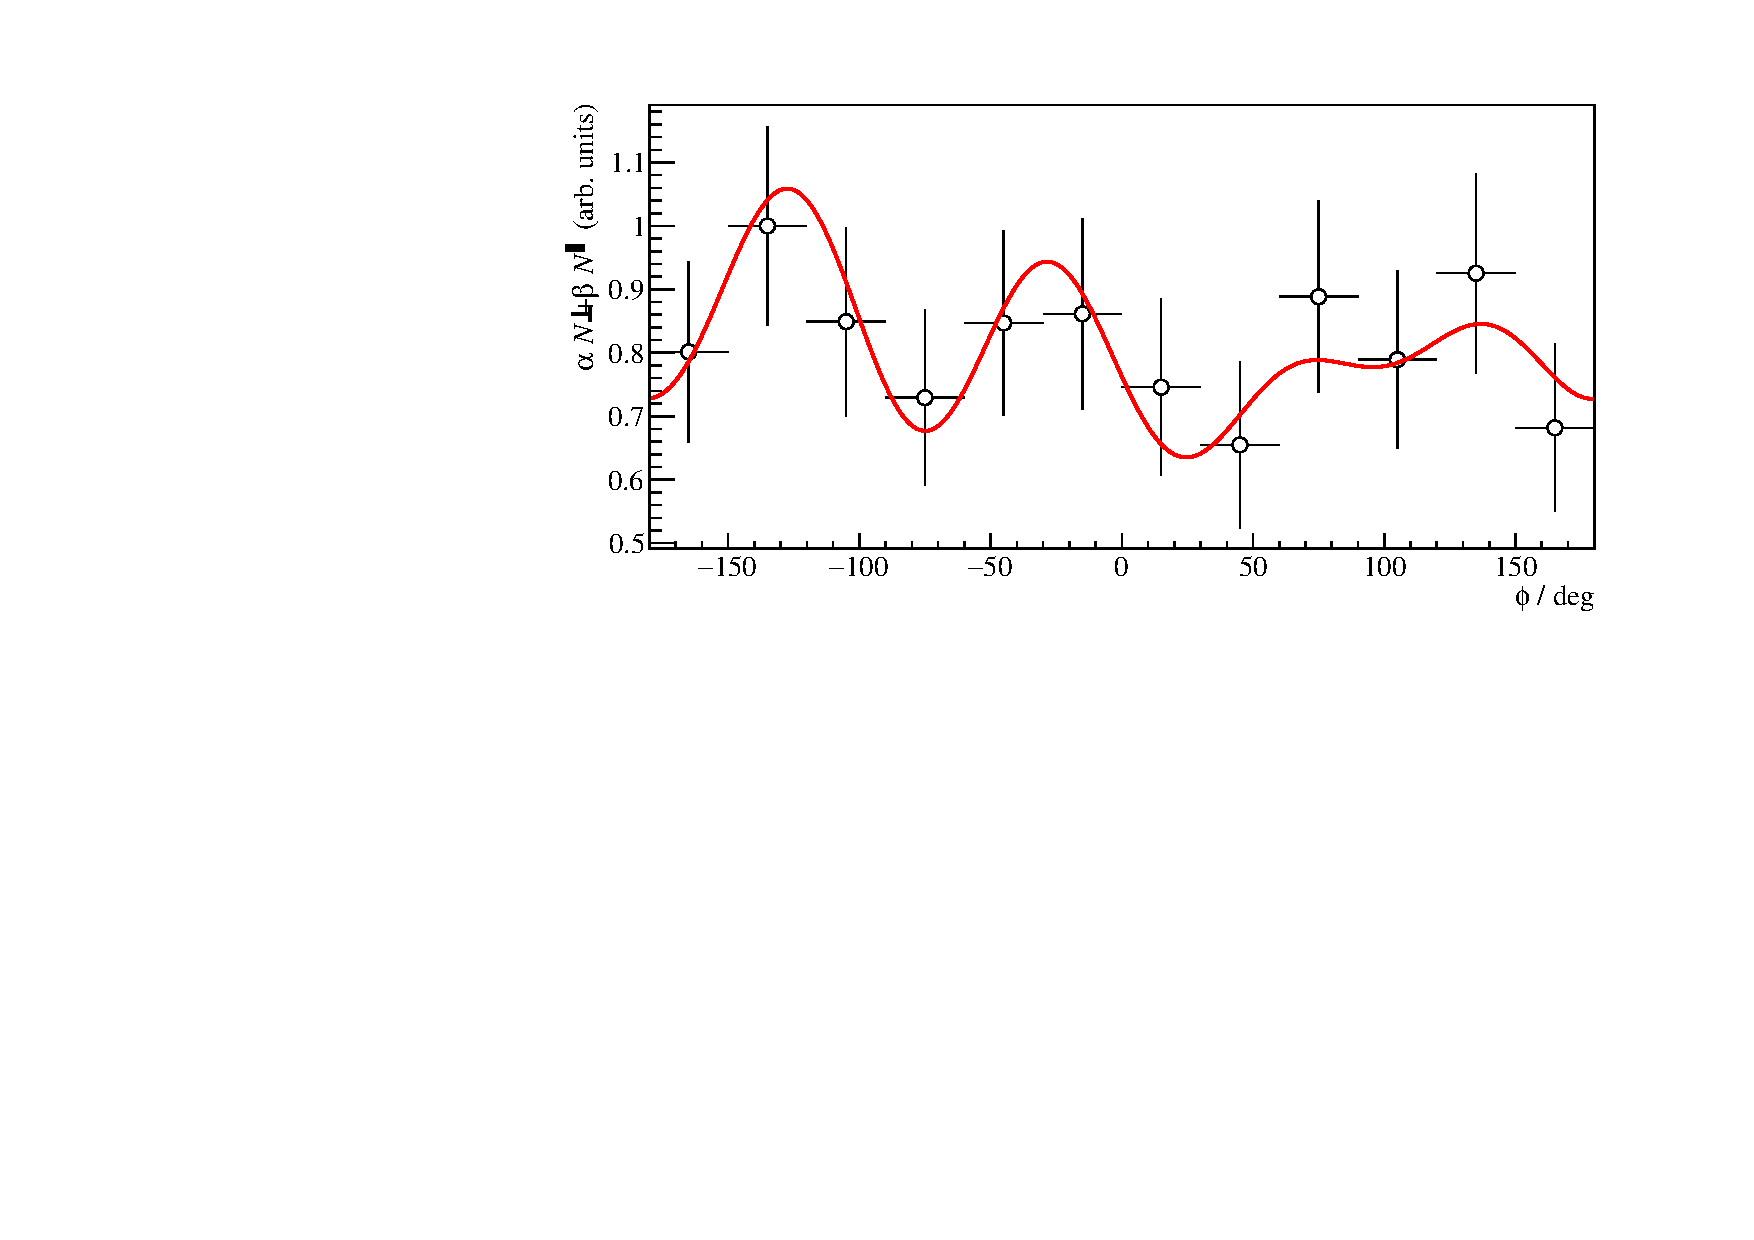
\includegraphics[width=\linewidth]{../RooFit/plots/toyMC_eff_unbinned_fit.pdf}
	\caption{Fitted efficiency function (red line) applied to the polarization weighted sum of event yields (data points) for one toy Monte Carlo bin. 12 bins in $\phi$ are built for demonstration.}
	\label{fig:toyMCeff}
\end{figure}
\subsubsection{Unbinned \textsc{Bayesian} fit}
When performing a \textsc{Bayesian} fit a systematic shift like Equation \eqref{eq:sigmeas} as result of background contributions is not easily applicable. The posterior distributions may be shifted by a constant value but including statistical errors of the background beam asymmetry is not possible. To circumvent this, the background beam asymmetry can be included inherently in the likelihood function that is part of the model being fitted. In practice, $\delta$ and $\Sigma_2$ have to be part of the data that is fed into the probabilistic model. In general though $\Sigma_2$ will have a statistical error, which can be included in the fashion of modeling \emph{missing data} \cite{stan}. Doing so, the value for $\Sigma_2$ is regarded as an estimate for the true, unknown (or missing) value $\Sigma_2^\text{true}$. The statistical error $\tau$ of $\Sigma_2$ specifies the measurement model assuming \textsc{Gaussian} errors 
\begin{equation}
	\Sigma_2^\text{true}\sim\mathcal{N}\left(\Sigma_2,\tau\right).
\end{equation}
 With this $\Sigma_2^\text{true}$ is added as an additional fit parameter to the probabilistic model, so that the  likelihood is modified as  
 \begin{equation}
 	\begin{aligned}
 		\ln\mathcal{L}&=\sum_{i=1}^{n}\ln p_\text{prompt}\left(\phi_i,p_{\gamma,i}\big|(1-\delta)\cdot\Sigma_1+\delta\cdot\Sigma_2^\text{true},a,b,\Sigma^\text{bkg}_t,a^\text{bkg}_t,b^\text{bkg}_t\right)\\&+\sum_{j=1}^m \ln p_\text{sideband}\left(\phi_j,p_{\gamma,j}\big|\Sigma^\text{bkg}_t,a^\text{bkg}_t,b^\text{bkg}_t\right).\label{eq:likalt}
 	\end{aligned}
 \end{equation}
For a complete inference $\Sigma_2^\text{bkg}$ also needs to be assigned a prior, which is chosen to be uniform to keep the number of fit parameters minimal. In total, 1000 bins in accordance with Table \ref{tab:mcsum1} are fitted with the adapted model that includes a background asymmetry $\Sigma_2$ with statistical error $\tau$ which are used to estimate the additional fit parameter $\Sigma_2^\text{true}$. For the sake of the toy Monte Carlo experiments the measurement error is arbitrarily chosen to be $\tau=0.05$ which is similar to the measured errors of the beam asymmetry in $2\pi^0$ photoproduction \cite{mahlbergphd}.


Figure \ref{fig:toyMCpost} shows the combined posteriors for the fit parameters $\Sigma_1$ and $\Sigma_t^\text{bkg}$ of the event based \textsc{Bayesian} fit for all generated toy Monte Carlo bins. The posteriors are added up since the truncation of the posteriors biases the results when combining them in a pooled likelihood model or normalized residuals $\Xi$. Previous experiments already proved sensible error estimation, i.e. distribution widths, when using the unbinned \textsc{Bayesian} fit. This is discussed in appendix \ref{app:trunc}. The input parameters are very well reproduced within the statistical error, which is given by the standard deviation of the \textsc{Gaussian}. The posterior distribution of $\Sigma_1$ is wider than the posterior of the background beam asymmetry $\Sigma_t^\text{bkg}$ because an additional measurement of $\Sigma_2$ with measurement error $\tau$ is used to estimate $\Sigma_1$. This is in complete analogy to shifting the point estimates $\Sigma^\text{meas}$ to their true values $\Sigma^\text{true}$, as described previously, which will also result in larger statistical error bars according to \textsc{Gaussian} error propagation.
\begin{figure}[htbp]
	\centering
	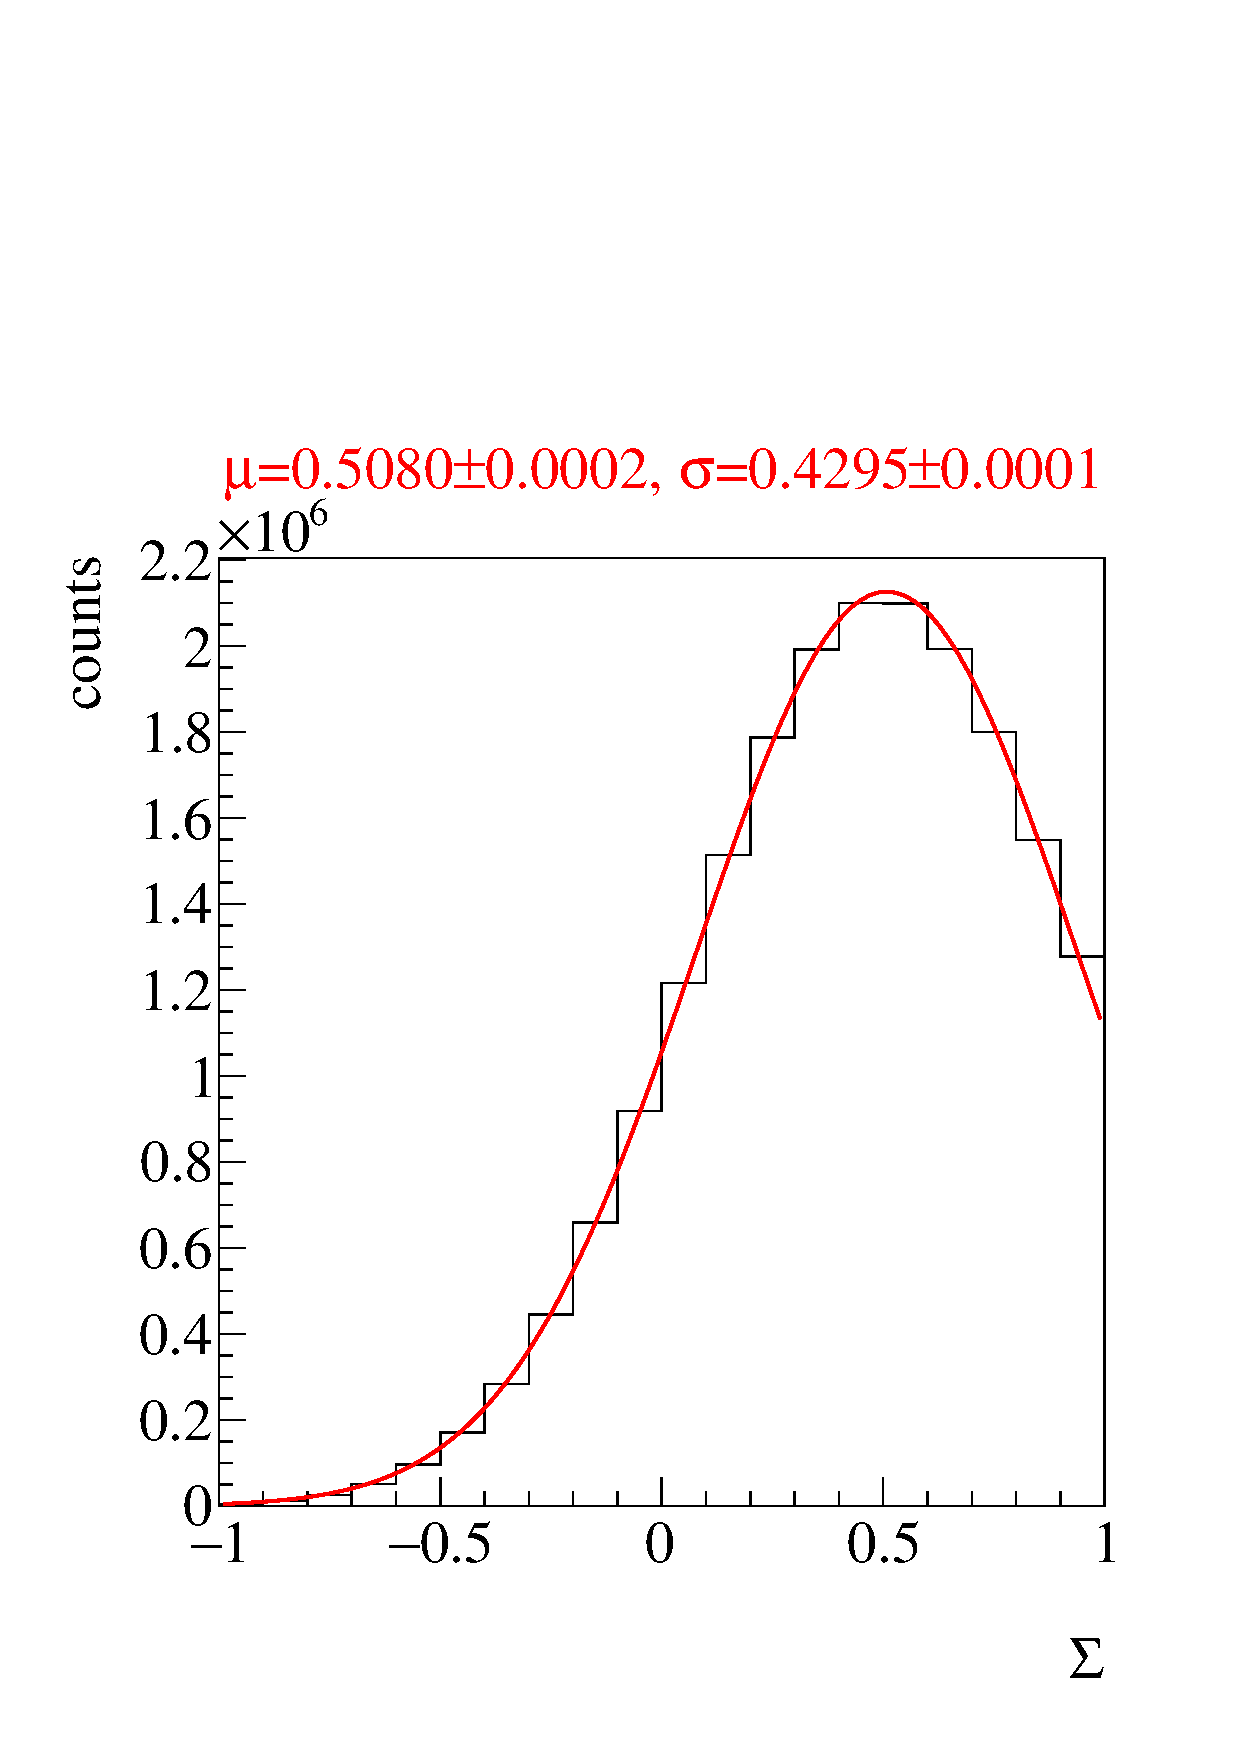
\includegraphics[width=.49\linewidth]{../bayes/etap_event_based_fit/plots/combined_post_add_raw.pdf}
	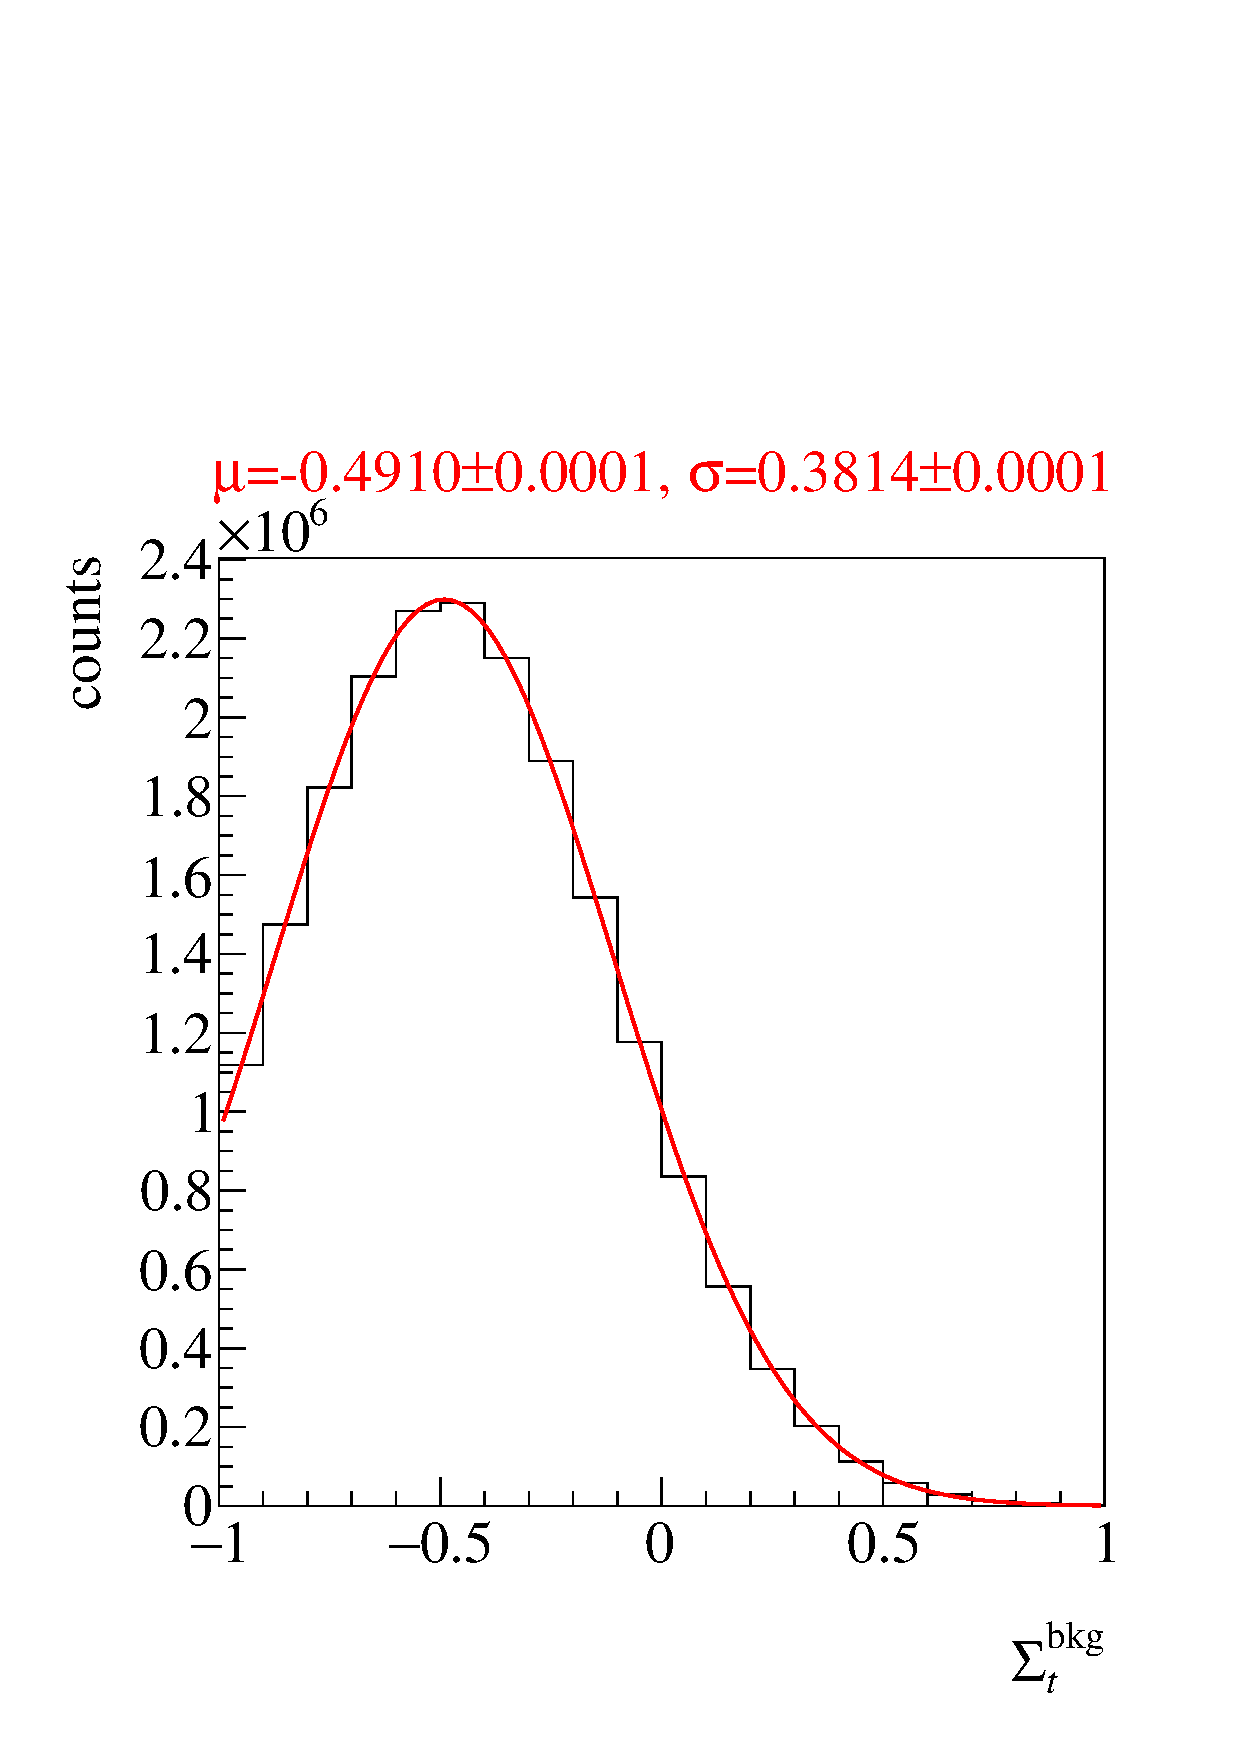
\includegraphics[width=.49\linewidth]{../bayes/etap_event_based_fit/plots/combined_post_add_raw_bkg.pdf}
	\caption{Combined (added) posteriors of all 1000 fits. Left: Signal beam asymmetry $\Sigma_1$ Right: Background beam asymmetry $\Sigma_t^\text{bkg}$. A \textsc{Gaussian} fit is performed with results given on top.}
	\label{fig:toyMCpost}
\end{figure}
Since the signal beam asymmetry $\Sigma_1$ was recognized correctly by the fit it is evident that the combined posterior distributions for $\Sigma_2$ are in full agreement with the expectations, see figure \ref{fig:toyMCpostalt}. Mean $\mu$ and standard deviation $\sigma$ are reproduced exactly as they were modeled as a \textsc{Gaussian} fit to the combined posteriors reveals.
\begin{figure}[htbp]
	\centering
	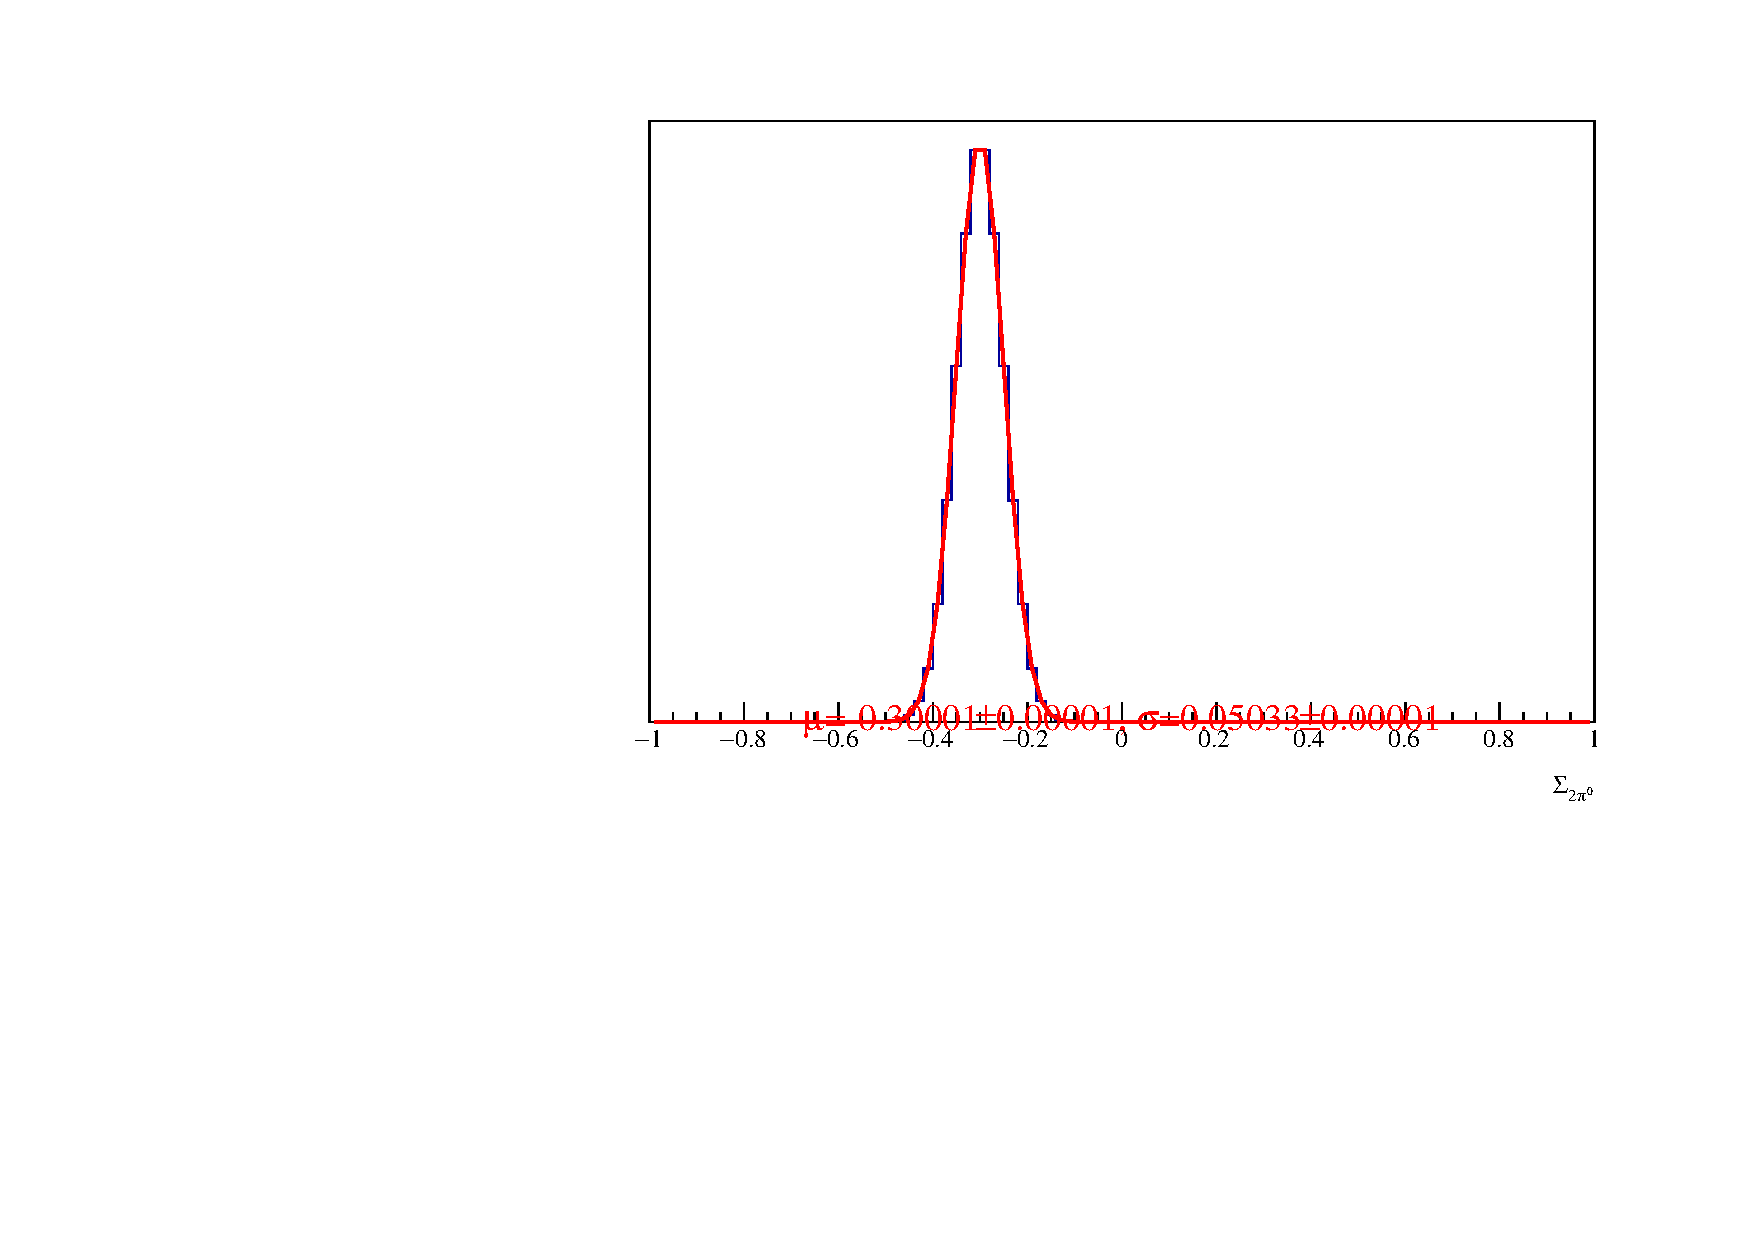
\includegraphics[width=.6\linewidth]{../bayes/etap_event_based_fit/plots/combined2pi0_post_add_raw.pdf}
	\caption{Combined (added) posteriors of all fits for the fit parameter $\Sigma_2^\text{true}$. A \textsc{Gaussian} fit is performed which reproduces exactly the values that were used for the simulations.}
	\label{fig:toyMCpostalt}
\end{figure}

\noindent It remains to investigate the properties of the employed \textsc{Markov} chains. First of all one observes that the accuracy of results, i.e. the relative MCSE, suffers from the available statistics which are significantly smaller in comparison with the previously investigated case for the $p\eta\to\gamma\gamma$ final state. Only $97\%$ of all unbinned fits fulfill the self set criterion of $\sigma_\text{MCSE}/\text{median}\left(p\left(\Sigma|y\right)\right)\leq0.05$ whereas for the toy Monte Carlo experiments in the previous section \ref{sec:sigmaeta} this was the case for \emph{all} unbinned fits. This observation however is not resembling a failing fit but rather the possibility for the data to mimic beam asymmetries close to zero because of the fewer available data points. In these cases the relative MCSE exceeds the threshold as has also been observed before. Convergence and full exploration of the available parameter space on the other hand is guaranteed for all fits because all $\widehat{R}$ values for all parameters and fits are within the demanded thresholds.


 Lastly, consistency of the fit results with the data that is fitted can be checked as before by a posterior predictive check of the detector coefficients $a,b$ plugged into the efficiency function $\epsilon\left(\phi\right)=\frac{1}{c}\cdot\left(\alpha \tilde{N}^\parallel + \beta\tilde{N}^\bot\right)$ as can be seen in Figure \ref{fig:toyMC_eff}. Each draw $a^{(s)},b^{(s)},s=1,\dots,20000$ is plotted as an opaque blue line. The mean over the posterior draws is indicated by the dashed line and follows the polarization weighted sum of event yields which is shown as data points. The mean agrees within statistical error bars at each point indicating finally a successful fit in every respect. 
 
It has been demonstrated that the chosen \textsc{Bayesian} model can describe data generated with two beam asymmetries very well. Note that expanding the existing model from before requires minimal changes since \emph{Stan} \cite{stan} allows modular implementations; only the new parameter $\Sigma_2^\text{true}$ and the new data points $(\Sigma_2,\tau,\delta)$ have to be added to give correctly centered posteriors that are not anymore systematically shifted. More effort would have to be made to get similar results with the traditional unbinned fitting method described before.


\begin{figure}[htbp]
	\centering
	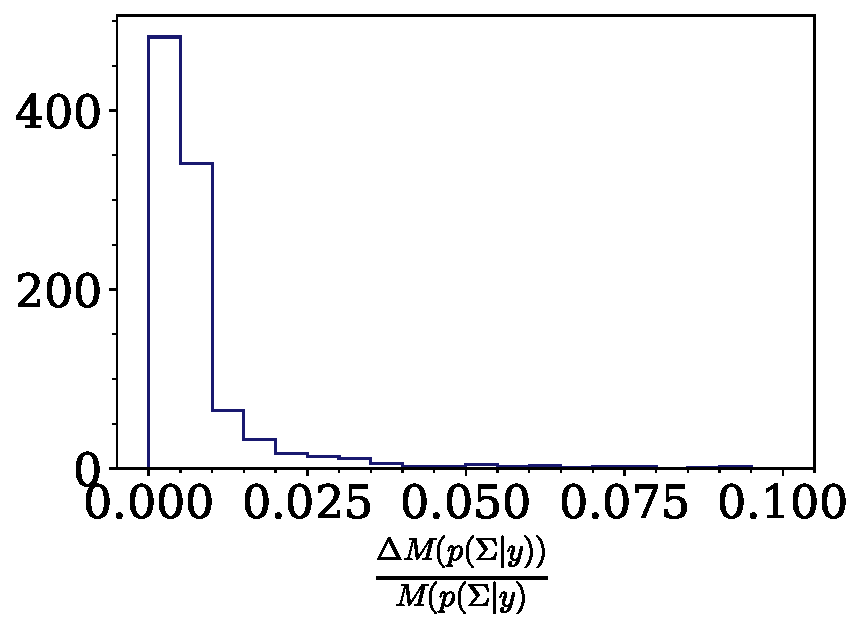
\includegraphics[width=.49\linewidth]{../bayes/etap_event_based_fit/plots/toyMC_mcse_hist.pdf}
	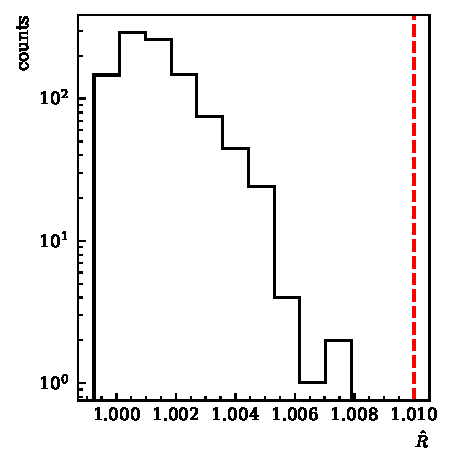
\includegraphics[width=.49\linewidth]{../bayes/etap_event_based_fit/plots/toyMC_rhat_hist.pdf}
	\caption{MCMC diagnostics for the event based \textsc{Bayesian} fit. Left: MCSE, Right: $\widehat{R}$-value. The critical values not to be exceeded are marked by the dashed lines.}
	\label{fig:toyMCdiagnostics}
\end{figure}
\begin{figure}[htbp]
	\centering
	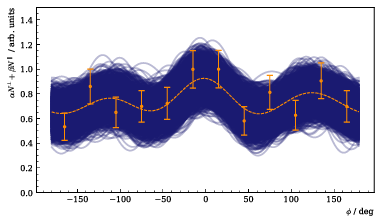
\includegraphics[width=\linewidth]{../bayes/etap_event_based_fit/plots/toyMC_eff_PPC.png}
	\caption{Posterior predictive checks of one toy Monte Carlo bin using the draws from the marginal posteriors of the detector coefficients $a,b$ (opaque blue lines). The mean values are marked by the dashed line and follow the distribution of the data points which are the polarization weighted sum of event yields, using 12 $\phi$ bins.}	
	\label{fig:toyMC_eff}
\end{figure}

\subsection{Application of event based fit to data}
Investigation of toy Monte Carlo experiments showed that the presence of polarized background events cause a systematic shift in the extracted beam asymmetry. The shift may be compensated by a modified likelihood function for the \textsc{Bayesian} fit or by reversing the shift \emph{after} obtaining intermediate results for $\Sigma^\text{meas}$ with an unbinned maximum likelihood fit. By studying Monte Carlo simulations of various mesonic final states it has been found that the main background contributions in the analysis of the final state $\gamma p \to p\eta'\to p\gamma\gamma$ is given by the false reconstruction of events $\gamma p \to p 2\pi^0\to p 4\gamma$, see chapter \ref{chap:events}. Conveniently, this includes the determination of the fraction of background events $\delta$, see Figure \ref{fig:bkg}. Furthermore, preliminary results for the beam asymmetry in double pion photoproduction at the CBELSA/TAPS experiment using the same binning as this analysis \cite{mahlbergphd} were available so that the previously discussed corrections can in fact be applied for each kinematic bin. It is hereby assumed that the \emph{entire} background is realized by $2\pi^0$ production and the fraction $\delta$ is determined by an according fit of Monte Carlo spectra. This holds true only approximately for each kinematic bin and is thus a source of systematic error, which is discussed in the next subsection \ref{subsec:sys}.

Figure \ref{fig:sigmaetap} shows the final results for the beam asymmetry in the reaction $\gamma p \to p\eta' \to p\gamma\gamma$ obtained from data taken at the CBELSA/TAPS experiment. Shown are two sets of results; the dark blue distributions are the results of a unbinned \textsc{Bayesian} without any modifications to the original model whatsoever. The dark orange data points are the corresponding results of an unbinned maximum likelihood fit $\Sigma^\text{meas}$. The light blue distributions however depict the results that were obtained from the modified \textsc{Bayesian} model, i.e. with the additional fit parameter $\Sigma_2^\text{true}$, the light orange data points correspond to the corrected point estimates $\Sigma^\text{true}$ according to Equation \eqref{eq:sigmeas}. In addition to the beam asymmetry $\Sigma_1=\Sigma_{\eta'}$ the fit also determines marginal posteriors for $\Sigma_2^\text{true}=\Sigma_{2\pi^0}$. To check consistency of the fit, these posterior distributions are compared to the results $\left(\Sigma_2,\tau\right)$ that were used as input \cite{mahlbergphd}, they are shown in Figure \ref{fig:sigma2pi0}. 

Several remarks can be made regarding these results:
\begin{enumerate}
	\item As it has been found studying toy Monte Carlo simulations, the modified \textsc{Bayesian} fit again successfully reconstructs two separate beam asymmetries. Figure \ref{fig:sigma2pi0} impressively shows the good agreement of input data points $\left(\Sigma_2,\tau\right)$ and posterior of $\Sigma_2^\text{true}$. On average $\Sigma_2\pm\tau$ covers $68\%$ of the posterior distributions, corresponding to a $1\sigma$ region, proving that no systematic error is made by introducing the additional fit parameter $\Sigma_2^\text{true}$.
	\item There is very good agreement between point estimates and corresponding posterior distributions. The point estimates give mean and standard deviation of the marginal posteriors to good approximation. If the point estimates are corrected according to Equation \eqref{eq:sigmeas} their statistical error increases. Similarly, the distributions from the modified \textsc{Bayesian} fit are wider, agreeing with the corrected point estimates and errors.
	\item Errors and distributions widths are rather large, which could be expected due to the small amount of events that could be used to extract the results. However, distributions are rarely truncated because they are mostly centered around $\Sigma\approx0$
	\item Shifting the final results of the beam asymmetry depending on the amount of background has marginal impact on the absolute scale. Although background contributions are far from negligible they exhibit only asymmetries close to $0$ (see Figure \ref{fig:sigma2pi0}). Thus, the shifted values still agree within statistical error bars or widths with the original values.
\end{enumerate}
\begin{figure}[htbp]
	\centering
	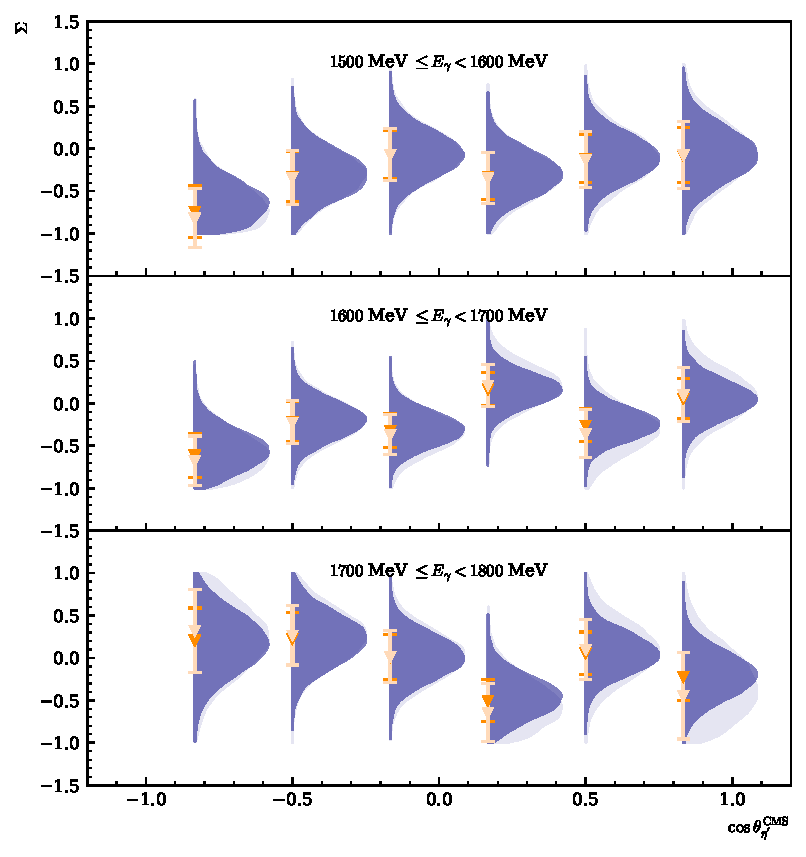
\includegraphics[width=\linewidth]{../bayes/etap_event_based_fit/plots/sigma_etap.pdf}
	\caption{Final results for the beam asymmetry $\Sigma$ in $\eta'$ photoproduction. Two sets of results are shown: The dark blue distributions and orange data points with errorbars are obtained with an unbinned fit that does not consider any background contributions. The light blue distributions and data points are obtained with the modified \textsc{Bayesian} fit and by correcting the point estimates according to Equation \eqref{eq:sigmeas}, respectively. All errors are statistical errors only.}
	\label{fig:sigmaetap}
\end{figure}
\begin{figure}[htbp]
	\centering
	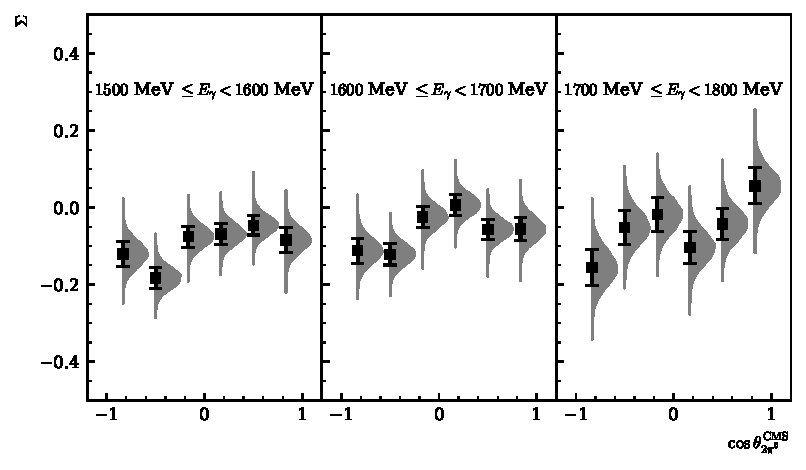
\includegraphics[width=\linewidth]{../bayes/etap_event_based_fit/plots/sigma_2pi0.pdf}
	\caption{Results for the additionally fitted $\Sigma_2^\text{true}$ (distributions) compared with the underlying data points \cite{mahlbergphd} with statistical errors. The error bars on average cover $1\sigma$ of the distributions, indicating a successful fit. All errors are statistical errors only.}
	\label{fig:sigma2pi0}
\end{figure}
To confirm between- and in-chain convergence for all fits, the $\widehat{R}$-values of all fit parameters are checked to be $1\lesssim\widehat{R}<1.05$. Due to the large number of samples this criterion is fulfilled without complications. Furthermore the relative MCSE with respect to the median of the posterior distributions is checked to confirm the accuracy of all chains. It is $\sigma_\text{mcse}/\text{median}\left(p(\Sigma|y)\right)\leq0.05$ for all but one fit where the beam asymmetry is very close to zero. Figure \ref{fig:etapdiagnostics} shows both quantities for all fits.

A last consistency check of the posterior predictive distributions of the efficiency function reveals no results aside from the expectations. Figure \ref{fig:etap_eff} shows all posterior predictive draws of the detector coefficients $a^{(s)},b^{(s)}$ plugged into the efficiency function $\epsilon\left(\phi\right)$. The mean of all draws describes the polarization weighted sum of event yields within statistical errors. The observed efficiency is less peaked than the simulated one (Figure \ref{fig:toyMC_eff}), confirming the results that have been found in section \ref{sec:sigmaeta}. Yet, more structures are observed compared to the $p\eta$ final state due to the decreased statistics.
\begin{figure}[htbp]
	\centering
	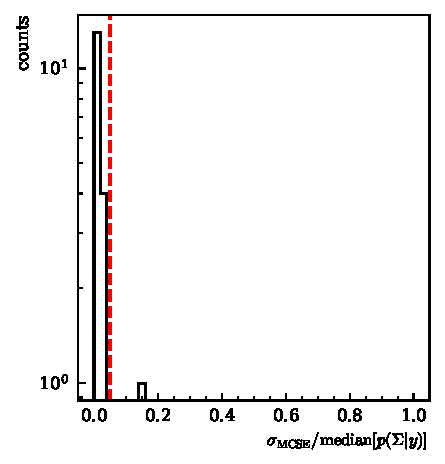
\includegraphics[width=.49\linewidth]{../bayes/etap_event_based_fit/plots/mcse_hist.pdf}
	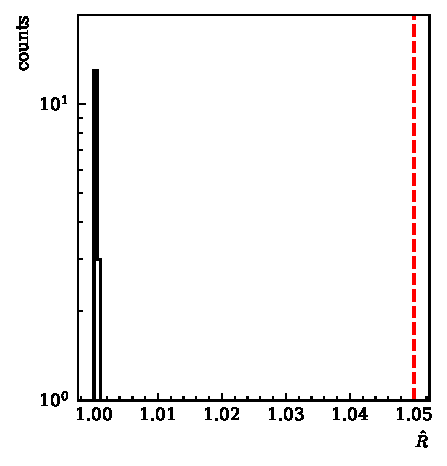
\includegraphics[width=.49\linewidth]{../bayes/etap_event_based_fit/plots/rhat_hist.pdf}
	\caption{MCMC diagnostics for the event based \textsc{Bayesian} fit. Left: MCSE, Right: $\widehat{R}$-value. The critical values not to be exceeded are marked by the dashed lines.}
	\label{fig:etapdiagnostics}
\end{figure}
\begin{figure}[htbp]
	\centering
	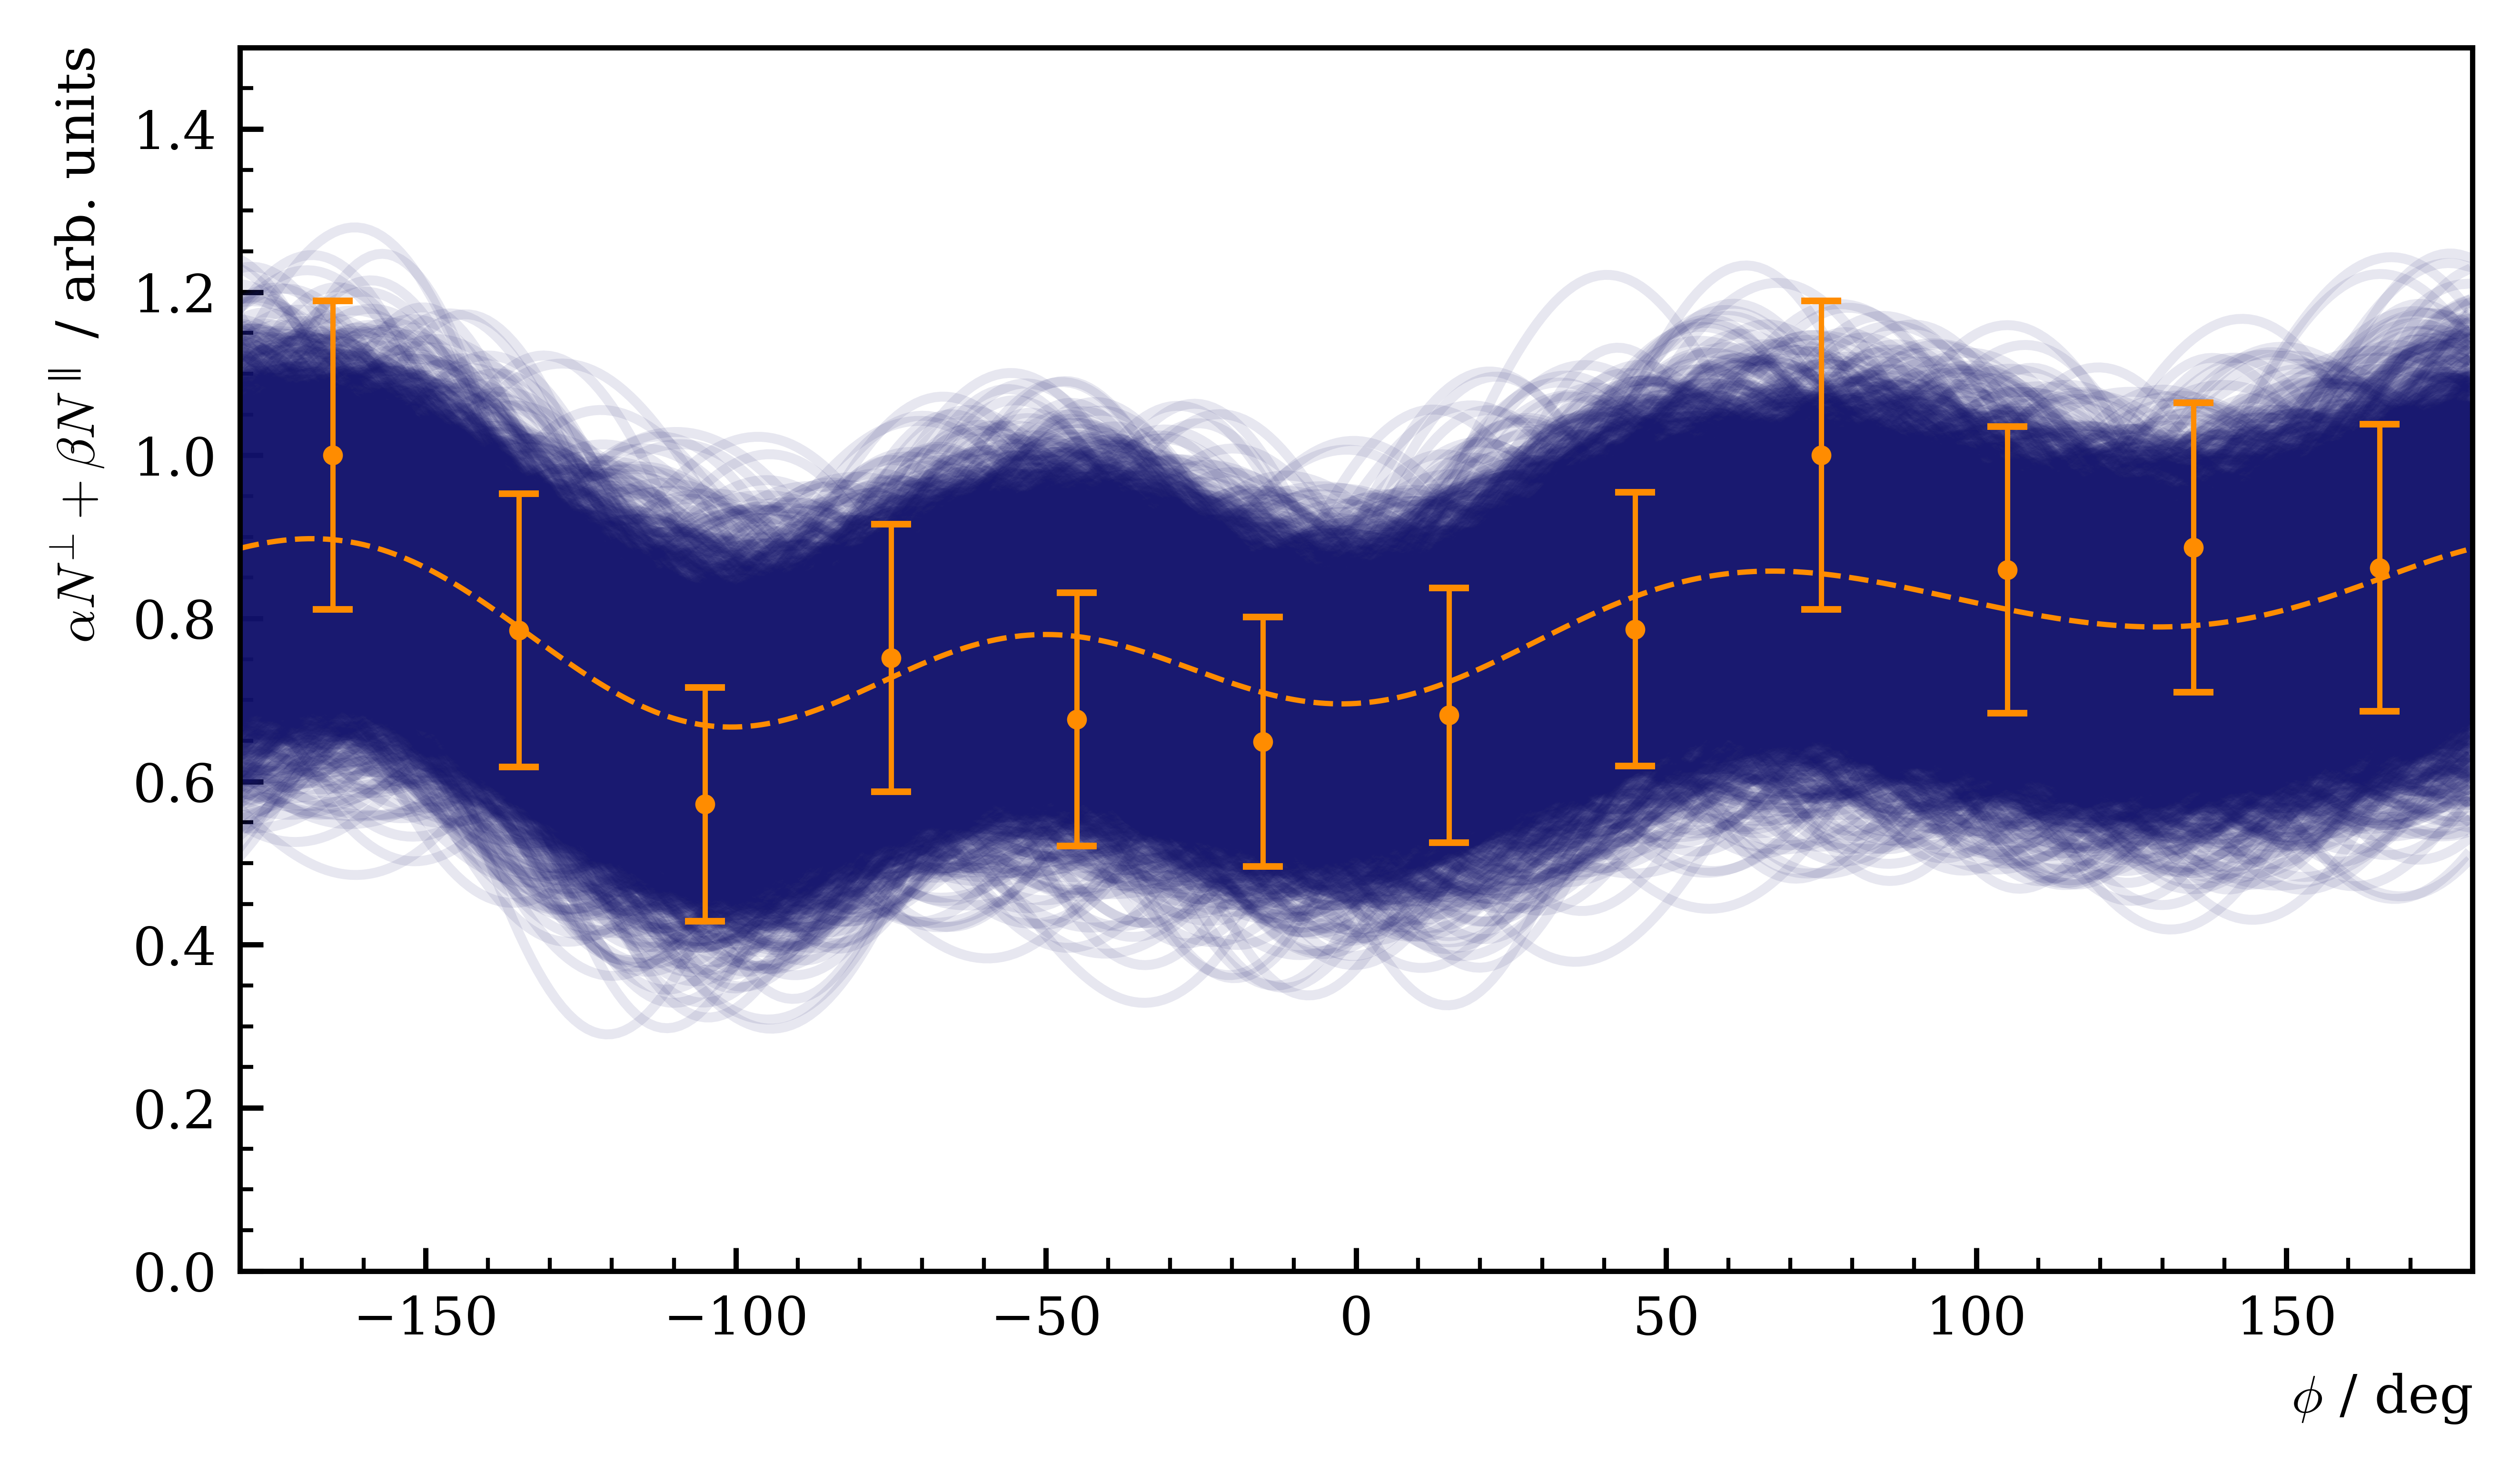
\includegraphics[width=\linewidth]{../bayes/etap_event_based_fit/plots/eff_PPC.png}
	\caption{Posterior predictive checks of the kinematic bin $\SI{1700}{\mega\eV}\leq E_\gamma<\SI{1800}{\mega\eV}, 0.67\leq\cos\theta<1$ using the draws from the marginal posteriors of the detector coefficients $a,b$ (opaque blue lines). The mean values are marked by the dashed line and follow the distribution of the data points which are the polarization weighted sum of event yields, using 12 $\phi$ bins.}	
	\label{fig:etap_eff}
\end{figure}
\subsection{Systematic error}
\label{subsec:sys}
There are two major sources for systematic error in the discussed analysis. On one hand, the determination of the polarization degree of the incident photon beam is not exactly accurate and thus influences the fit results which heavily depend on the linear polarization degree. On the other hand, neglecting polarized background events originating from a different reaction that have been falsely regarded as $2\pi^0$ events when shifting the intermediate results may create systematic errors. 

The relative error of the polarization degree can be estimated during the determination process where analytically calculated bremsstrahlung spectra (ANB) are fitted to measured spectra \cite{farahphd}. This allows to give the relative error in the beam energy region that was analyzed as \cite{farahphd}
\begin{equation}
	\frac{\Delta p_\gamma}{p_\gamma}=
	\begin{cases}
		0.05,& \text{ if } E_\gamma<\SI{1600}{\mega\eV}\\
		0.08,& \text{ otherwise. }
	\end{cases}
\end{equation}
It was assumed that 
\begin{equation}
	\Sigma^\text{meas}=\left(1-\delta\right)\cdot\Sigma^\text{true}+\delta\Sigma^\text{bkg},
\end{equation}
with $\Sigma^\text{true}=\Sigma_{\eta'}$ and $\Sigma^\text{bkg}=\Sigma_{2\pi^0}$ and according modifications to the obtained results have been made. However, regarding the entire background contributions to double pion photoproduction holds only approximately in each bin. Actually, the measured value for the beam asymmetry is given by \begin{equation}
\Sigma^\text{meas}=\left(1-\delta_1-\delta_2\right)\cdot\Sigma_{\eta'}+\delta_1\Sigma_{2\pi^0}+\delta_2\Sigma^\text{r bkg},
\end{equation}
where $\delta_1$ is the relative contribution of $2\pi^0$ production events and $\delta_2$ the relative contribution of other background events, e.g. $\pi^0\eta$ production, that have been neglected before that may exhibit an asymmetry $\Sigma^\text{r bkg}$. The systematic uncertainty of $\Sigma_{\eta'}$ can then be determined by setting $\Sigma^\text{r bkg}=\pm1$ and determining the maximum deviation from the previous results. The results from the unbinned maximum likelihood fit are used which to good approximation also give the median and mean of the posterior distributions.
\begin{equation}
	\Delta\Sigma_{\eta'}=\text{max}\left[\left|\frac{\Sigma^\text{meas}-\delta_1\cdot\Sigma_{2\pi^0}\pm\delta_2\cdot1}{1-\delta_1-\delta_2}-\frac{\Sigma^\text{meas}-\delta\cdot\Sigma_{2\pi^0}}{1-\delta}\right|\right]
\end{equation}
The two fractions $\delta_1$ and $\delta_2$ are determined by fitting the invariant mass spectra of Monte Carlo data bin-wise to the measured data for each kinematic bin, as described in chapter \ref{chap:events}. Hereby $\delta_2$ is determined by subtracting the background fraction $\delta_1$ obtained from a fit that only allowed $2\pi^0$ contributions underneath the $\eta'$ invariant mass peak from the background fractions $\delta$ obtained fitting \emph{all} MC spectra to the data. The total absolute systematic error is then given by
\begin{equation}
	\Delta\Sigma_{\eta'}^\text{sys}=\sqrt{\left(\frac{\Delta p_\gamma}{p_\gamma}\Sigma_{\eta'}\right)^2+\left(\Delta\Sigma_{\eta'}\right)^2}.
\end{equation}
Figure \ref{fig:etapsys} shows all results with systematic uncertainites given on the bottom of each plot.

\begin{figure}[htbp]
	\centering
	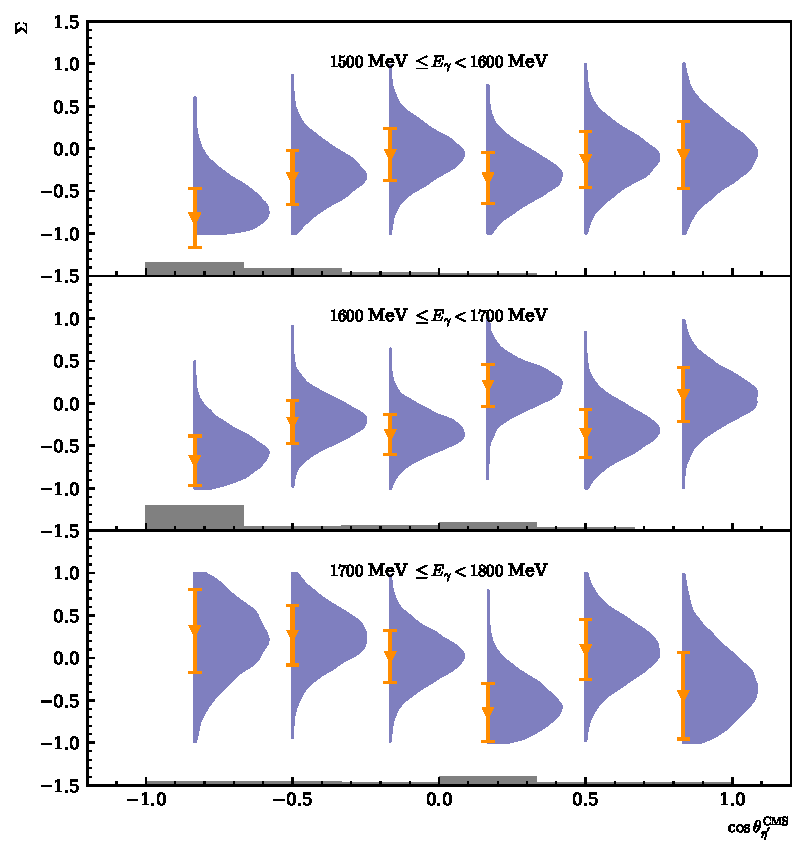
\includegraphics[width=\linewidth]{../bayes/etap_event_based_fit/plots/sigma_etap_sys.pdf}
	\caption{Final results for the beam asymmetry $\Sigma_{\eta'}$ for all energy and angular bins. Only the corrected results from the unbinned maximum likelihood fit and distributions from the modified \textsc{Bayesian} fit are shown. The bottom of each plot indicates the systematic error as gray bars. It was determined as previously discussed.}
	\label{fig:etapsys}
\end{figure}
